\documentclass[11pt]{article}
\usepackage[T1]{fontenc}
\usepackage[utf8]{inputenc}
\usepackage{lmodern}
\usepackage[a4paper,margin=29mm]{geometry}
\usepackage{amsmath,amssymb,amsthm,mathtools}
\usepackage{booktabs,array,graphicx}
\usepackage{microtype}
\usepackage[numbers,sort&compress]{natbib}
\usepackage[colorlinks=true,linkcolor=blue,citecolor=blue,urlcolor=blue]{hyperref}
\newtheorem{theorem}{Theorem}[section]
\newtheorem{proposition}[theorem]{Proposition}
\newtheorem{lemma}[theorem]{Lemma}
\newtheorem{corollary}[theorem]{Corollary}
\theoremstyle{definition}
\newtheorem{definition}[theorem]{Definition}
\newtheorem{example}[theorem]{Example}
\theoremstyle{remark}
\newtheorem{remark}[theorem]{Remark}
\newcommand{\R}{\mathbb R}
\newcommand{\N}{\mathbb N}
\newcommand{\Acal}{\mathcal A}
\newcommand{\Wcal}{\mathcal W}
\newcommand{\Pcal}{\mathcal P}
\newcommand{\norm}[1]{\left\lVert#1\right\rVert}
\DeclareMathOperator{\OPT}{OPT}
\DeclareMathOperator{\argmin}{argmin}
\DeclareMathOperator{\argmax}{argmax}

\title{Rounding switching controls under a hard switch budget:\\sharp minimax bounds and exact algorithms}
\author{}
\date{}
\begin{document}
\maketitle
\begin{abstract}
We study cumulative-error rounding of measurable simplex-valued controls when
the integer control has a hard bound on its number of switches. We determine
the continuous minimax error through three switches whenever the number of
modes exceeds the number of activation blocks. A heavy-mode reduction and
sharp one-sided reach bounds give matching extremizers; the four-block proof
uses exact certificates covering every mode count. Mode removal yields
general-budget bounds, enlarged exact plateau ranges, and the sharp first
mode-count correction to the dimension-free limit. On finite grids we derive
an explicit arbitrary-grid one-switch minimax formula and exact three-mode
values from a complete floor-history representation. These include the
continuous boundary value with two switches and counterexamples to specific
published finite-grid claims. For an input with $n$ modes on $N$ grid cells,
we give an exact one-switch algorithm using $O(nN)$ rational operations
and a fixed-budget subset algorithm with linear arithmetic
dependence on the number of modes. A sharp switch-preserving grid transfer
provides additive coarse-grid certificates with quantified input perturbation.
Exact rational checks and reproducible public-profile computations accompany
the proofs.
\end{abstract}
\section{Introduction}\label{sec:introduction}

In the combinatorial integral approximation (CIA) decomposition of
mixed-integer optimal control~\cite{sager2011cia}, a relaxed control that may
divide activity among several modes is rounded to an integer control that
activates one mode at a time. The rounding error is the largest absolute
difference between the cumulative mode allocations of the two controls; under
regularity assumptions it bounds the resulting state
error~\cite{sager2011cia,zeile2022decomposition}. Without switching
restrictions, sum-up rounding makes this error proportional to the grid width,
so it vanishes under refinement~\cite{sager2011cia,kirches2020tight}. With a
hard bound on the number of switches it does not~\cite{sager-zeile2021}:
refinement only improves the placement of finitely many switches and cannot
remove the error caused by the budget itself. The relevant questions are
therefore quantitative: what error is unavoidable, which relaxed inputs attain
it, and how can one compute an optimal or certifiably near-optimal schedule
for a given input?

We answer these questions for measurable simplex-valued controls on a horizon
$[0,T]$, with $n$ modes and at most $s$ switches, that is, at most $k=s+1$
activation blocks. The initial mode is free, repeated modes are allowed, and
the default model has no dwell or transition restrictions. For an input
cumulative allocation $A$, write $\OPT_s(A)$ for the smallest cumulative
discrepancy among continuous-time schedules and $F_{n,s}(T)=\max_A\OPT_s(A)$
for its worst-case value. A superscript $\mathcal T$ restricts switching times
to a grid $\mathcal T$.

\subsection{Main results}

\paragraph{Sharp continuous minimax values.}
Our main formula (Theorem~\ref{thm:small-full}) is
\begin{equation}\label{eq:intro-main}
 F_{n,s}(T)=T\max\left\{\frac{1}{s+2},
 \frac{1}{n\bigl((n/(n-1))^{s+1}-1\bigr)}\right\},
 \qquad 0\le s\le3,\quad n\ge s+2.
\end{equation}
The first term is attained by $s+2$ successive pure modes of equal duration.
The second is the sharp one-sided error of the uniform input on all $n$
modes. It exceeds the first from $n=5,8,12$ onward for $s=1,2,3$,
respectively (Figure~\ref{fig:minimax-regimes}). Thus the continuous lower
bound $T/(s+2)$ of Sager and Zeile~\cite[Proposition~4]{sager-zeile2021} is
the exact value for $s+2\le n\le4,7,11$ and is exceeded for larger $n$,
contrary to their remark that this bound cannot be
improved~\cite[p.~615]{sager-zeile2021}. The
formula covers all measurable inputs, and its lower bound allows competing
schedules to repeat modes.

\begin{figure}[tb]
\centering
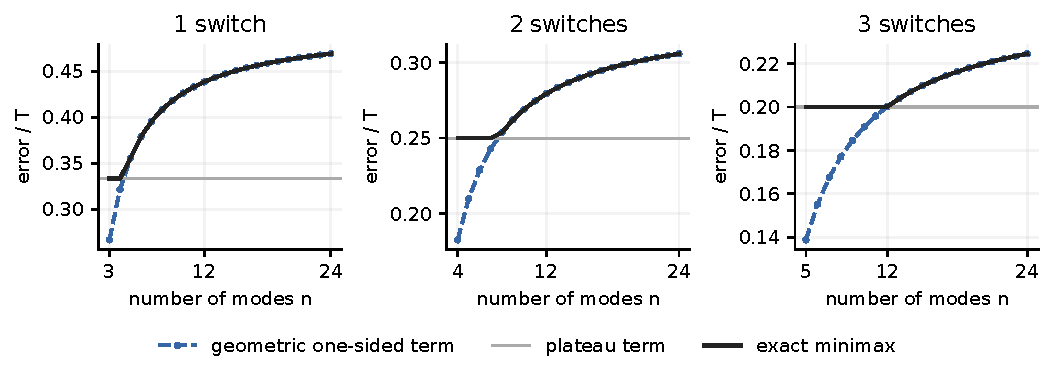
\includegraphics[width=\linewidth]{figures/minimax-regimes.pdf}
\caption{The exact continuous minimax value divided by $T$, its plateau term, and
the geometric one-sided uniform term
for one, two, and three switches, on their stated mode ranges. Lines connect
integer mode counts.}
\label{fig:minimax-regimes}
\end{figure}

The proof separates heavy modes from a one-sided problem. If some terminal
mode mass exceeds $E$ and $T\le(s+2)E$, integral-prefix rounding followed by
a reordering at the first repeated mode gives an $s$-switch schedule with
full error at most $E$, for every $n$ (Theorem~\ref{thm:heavy}). Otherwise
only the one-sided error matters (Theorem~\ref{thm:one-sided-reduction}),
and we prove sharp reach bounds for schedules with up to four distinct modes.
The two- and three-block arguments are analytic
(Lemma~\ref{lem:reach-two}, Theorem~\ref{thm:reach-three}); the four-block
bound (Theorem~\ref{thm:reach-four}) is computer-assisted, using exact
rational and polynomial dual certificates for a necessary-condition linear
program after a symmetry reduction, for every $n\ge5$. The spare-mode
hypothesis $n>k$ cannot simply be dropped: at $n=k=3$ a constructed input
has an exact three-block one-sided optimum strictly worse than the uniform
input, even when modes may repeat (Proposition~\ref{prop:three-mode-failure}).

\paragraph{General budgets.}
For every $k=s+1<n$, removing a largest-mass or a smallest-mass mode carries
one-sided bounds from $n-1$ modes and $k-1$ blocks to $n$ modes and $k$
blocks (Lemma~\ref{lem:mode-removal}).
This gives a closed upper coefficient (Theorem~\ref{thm:general-coefficient}),
a sharper bound seeded by the four-block theorem (Theorem~\ref{thm:seeded}),
the plateau value $F_{n,k-1}(T)=T/(k+1)$ at least for
$k+1\le n\le\max\{2k,k(k+1)/2\}$ (Corollaries~\ref{cor:general-plateau}
and~\ref{cor:light-boundaries}), and
\[
 F_{n,k-1}(T)=\frac{T}{k}-\frac{(k+1)T}{2kn}
                  +O_k(Tn^{-2})\qquad(n\to\infty)
\]
(Proposition~\ref{prop:general-asymptotics}). The leading dimension-free
term $T/k$ already follows from classical integral-prefix rounding
(Proposition~\ref{prop:dimension-free}); the first mode-count correction is
sharp. Inputs with equal terminal masses have stronger guarantees, including
the exact instance value $T/n$ in a band next to $n=k$
(Corollary~\ref{cor:light-boundaries}). The exact reach bound for five or
more blocks remains open; Appendix~\ref{sec:higher-reach} isolates the
missing inequality, and no other result depends on it.

\paragraph{Exact finite-grid values.}
On an arbitrary grid with $N$ cells and $n\ge3$, the one-switch minimax value
is an explicit maximum over $O(N^2)$ closed-form candidates, evaluable in
$O(N^2)$ rational operations for rational grid data; a worst input has two
component types and at most three time phases
(Theorem~\ref{thm:finite-one}). For three modes on
unit grids, a complete description of the realizable floor histories
(Proposition~\ref{prop:floor-automaton}), valid for every grid length, gives
exact values on five, six, and seven cells
(Theorems~\ref{thm:five-cells} and~\ref{thm:seven-cells},
Corollary~\ref{cor:six-cells}), including
$F^{\mathrm{unit}}_{3,3}(7)=4/3$. The five- and six-cell values give the
upper bounds in $F_{3,2}(T)=T/5$ (Corollary~\ref{cor:three-two-continuous})
and $T/7\le F_{3,3}(T)\le T/6$; the lower bounds are the case $n=3$ of
\cite[Proposition~4]{sager-zeile2021}. The exact value of $F_{3,3}$ remains
open. Together with the uniform-input examples of
Section~\ref{sec:one-switch}, these results disprove three specific
finite-grid statements of \citet{sager-zeile2021}: the first branch of their
Conjecture~1 fails even as an upper bound
(Examples~\ref{ex:five-mode-conjecture} and~\ref{ex:three-cell-conjecture}),
the equality in its second branch fails on seven cells, and the lower bound
in their Corollary~5 fails on five cells
(Section~\ref{sec:floor-chambers}).

\paragraph{Exact algorithms for a given input.}
For a supplied input on $N$ grid cells, three candidate mode pairs per grid
boundary suffice for one switch, which gives an exact $O(nN)$ algorithm
(Theorem~\ref{thm:linear-one-switch}). For a fixed budget, enumerating the
block boundaries and assigning blocks to modes by a subset dynamic program
gives an exact algorithm whose arithmetic cost is polynomial in $N$ for each
fixed $s$ and linear in $n$ (Theorem~\ref{thm:fixed-budget}). It allows
repeated modes and can enforce mode-specific minimum dwell times on maximal
runs. For piecewise-affine input and switches anywhere in time, a finite
family of rational linear programs gives the continuous instance optimum
exactly (Section~\ref{sec:algorithms}).

\paragraph{Sharp grid transfer and certified coarsening.}
A chronological, support-preserving rounding moves any finitely switching
schedule to a uniform grid of width $h$ without adding switches and changes
cumulative occupations by strictly less than $h$
(Theorem~\ref{thm:sharp-transfer}). Hence
$\OPT_s(A)\le\OPT^{\mathcal T}_s(A)<\OPT_s(A)+h$, with the analogous
minimax inequality (Corollary~\ref{cor:opt-transfer}); the coefficient one
is sharp uniformly over modes and budgets
(Proposition~\ref{prop:transfer-sharpness}). Exact optimization on a coarse
uniform grid therefore returns a feasible schedule together with a certified
additive interval for the continuous optimum
(Theorem~\ref{thm:certified-coarsening}), with explicit bounds for input
quantization (Corollary~\ref{cor:coarse-perturbation}). Dwell constraints
need separate treatment: an elementary example keeps a fixed positive gap on
arbitrarily fine odd grids (Example~\ref{ex:dwell-grid-gap}).

\paragraph{Computations and verification.}
Section~\ref{sec:computations} applies these methods in exact rational
arithmetic to a public three-mode Lotka--Volterra relaxed control on 12,000
cells~\cite{pycombina-data}. For the quantized input, the exact one-switch
optimum on the full grid is $1.889$, against the continuous optimum
$1.8885876$, and a 48-cell coarse grid brackets the continuous three-switch
optimum in an interval of width $0.25$. Separate Lean developments verify the arbitrary-grid one-switch formula, the transfer and
coarsening results with their supporting instance algorithms, the exact
five-, six-, and seven-cell three-mode values, and $F_{3,2}(T)=T/5$;
Section~\ref{sec:discussion} states their scope.

\begin{table}[tb]
\centering\small
\caption{Main scopes. Here $k=s+1$, and a unit grid has horizon $N$.}
\label{tab:results-synopsis}
\begin{tabular}{@{}p{.32\linewidth}p{.43\linewidth}p{.18\linewidth}@{}}
\toprule
Problem & Result & Reference\\
\midrule
Continuous minimax, $0\le s\le3$, $n\ge s+2$
 & Exact formula~\eqref{eq:intro-main} & Theorem~\ref{thm:small-full}\\
General budgets, $n>k$ & Closed and seeded upper bounds; sharp first correction
 & Section~\ref{sec:general-budgets}\\
Three-mode boundaries & $F_{3,2}=T/5$; $T/7\le F_{3,3}\le T/6$
 & Section~\ref{sec:floor-chambers}\\
One-switch grid minimax, $n\ge3$ & Explicit formula on arbitrary grids
 & Theorem~\ref{thm:finite-one}\\
Three-mode unit grids & $(N,s)=(5,2),(6,3),(7,3)$: values $1,1,4/3$
 & Section~\ref{sec:floor-chambers}\\
Supplied grid input & Exact one-switch and fixed-budget algorithms
 & Section~\ref{sec:algorithms}\\
Continuous-to-grid transfer & Sharp uniform coefficient; additive certificates
 & Section~\ref{sec:transfer}\\
\bottomrule
\end{tabular}
\end{table}

\subsection{Relation to earlier work}

Sager, Jung, and Kirches~\cite{sager2011cia} introduced the CIA decomposition
and the switch-constrained rounding subproblem, with a mixed-integer linear
formulation and a tailored branch-and-bound algorithm. Sager and
Zeile~\cite{sager-zeile2021} study a total-variation constraint on the
integer control, develop maximum dwell rounding, and give the worst-case
bounds and conjecture compared above; Sections~\ref{sec:one-switch}
and~\ref{sec:floor-chambers} compare their finite-grid statements in
detail.

Integral flow and matching are established tools for rounding partial sums;
Knuth's two-way rounding theorem~\cite{knuth1995} is a classical example.
Bestehorn and Kirches~\cite[Corollary~2.7]{bestehorn2021vanishing} prove
support-preserving CIA rounding with discrepancy at most one uniform grid
width. Our transfer proof gives this construction explicitly and adds the
chronological argument that preserves a supplied schedule's switch count,
the strict bound, and a sharp instance-wise discretization family.
Section~\ref{sec:transfer} also gives a counterexample to the unrestricted
instance-wise reading of the half-grid argument preceding their
Conjecture~1~\cite[p.~615]{sager-zeile2021} (see also
\cite[p.~139]{zeile2021thesis}), which is not stated as a theorem.

Exact graph algorithms for switching costs, minimum dwell times, and support
restrictions already exist. The shortest-path formulation of Bestehorn,
Hansknecht, Kirches, and Manns~\cite{bestehorn2021shortest} gives
switching-cost-aware rounding (SCARP), with a complexity bound exponential in
the mode count. Zeile, Robuschi, and Sager~\cite{zeile2021dwell} analyze
minimum dwell rounding, and switching-time enumeration is discussed in
\cite[Section~6.4.3]{zeile2021thesis}. Abbasi-Esfeden, Plate, Sager, and
Swevers~\cite{abbasi2025} propose a dynamic-programming-inspired CIA method
with dwell constraints; they state that it does not guarantee global
optimality in general, because optimal substructure is lost. What is
specific to our exact algorithms is the CIA dominance and subset reduction,
with its proved linear dependence on the mode count for a fixed budget.

Several approximation results concern grids whose refinement lets the number
of switches grow: tight sum-up rounding bounds~\cite{kirches2020tight},
compactness and convergence of CIA decompositions~\cite{kirches2021compact},
and adaptive nonuniform refinement for SCARP~\cite{bestehorn2023adaptive}.
Our coarsening certificate instead concerns the best approximation under a
fixed switch budget, to a prescribed additive accuracy, including exact
integration across nonaligned input and output grids. It does not assert
convergence to the relaxed control at fixed budget. Our results concern
discrepancy, switching feasibility, and computational cost only;
consequences for states or objectives of an underlying control problem
require its dynamics and the regularity assumptions of
\cite[Theorem~1 and Corollary~1]{zeile2022decomposition}.

\subsection{Organization}

Section~\ref{sec:foundations} defines the model.
Sections~\ref{sec:one-switch}--\ref{sec:structural-limits} prove the
continuous results through three switches and show where the constructions
stop, and Sections~\ref{sec:general-budgets}--\ref{sec:predecessors} treat
general budgets. Sections~\ref{sec:finite-one}--\ref{sec:floor-chambers}
give the finite-grid values, Sections~\ref{sec:algorithms}
and~\ref{sec:transfer} the instance algorithms and certificates, and
Section~\ref{sec:computations} the computations.
Section~\ref{sec:discussion} discusses open questions;
Appendix~\ref{sec:higher-reach} treats the higher-reach question.

\section{Problem and basic properties}\label{sec:foundations}

We use the setting of~\cite{sager-zeile2021}.

\subsection{Controls, schedules, and the two error criteria}

Fix a horizon $T>0$ and an integer number of modes $n\ge2$. Throughout,
switch budgets $s$ are nonnegative integers, activation-block counts $k$ are
positive integers, and grid sizes $N$ are positive integers. Write
$[n]=\{1,\ldots,n\}$ and
\[
 \Delta_n=\left\{a\in\R^n:a_i\ge0,\ \sum_{i=1}^n a_i=1\right\}.
\]
A relaxed control is a Lebesgue-measurable map
$\alpha:[0,T]\to\Delta_n$, considered up to equality almost everywhere.
Its cumulative allocation and terminal masses are
\begin{equation}\label{eq:cumulatives}
 A_i(t)=\int_0^t\alpha_i(u)\,du,\qquad m_i=A_i(T).
\end{equation}
Thus $A_i$ is nondecreasing and $1$-Lipschitz, $A_i(0)=0$, and
$\sum_i A_i(t)=t$. Conversely, every vector of functions with these properties
is the cumulative allocation of such a control: Lipschitz functions are
absolutely continuous and differentiable almost everywhere, their derivatives
are nonnegative, and differentiation of the sum gives a simplex-valued
vector almost everywhere. Denote this class of cumulative allocations by
$\Acal_n(T)$. We use either $\alpha$ or $A$ to specify an input.

An integer control, or schedule, selects a coordinate vector $e_i$ on each of
finitely many intervals. Its initial activation is free: only changes between
two successive active modes count as switches. Its values at isolated times
are immaterial. Let $\Wcal_{n,k}(T)$ be the set of cumulative occupations
\[
 W_i(t)=\int_0^t\omega_i(u)\,du
\]
of schedules with at most $k$ positive-length activation blocks, equivalently
at most $s=k-1$ switches. Unless explicitly stated otherwise, repeated modes
are allowed, the initial and final modes are unrestricted, and there are no
dwell-time or transition restrictions. A parameterization of this entire set
uses a word $p\in[n]^k$ and ordered times
\begin{equation}\label{eq:schedule-parameterization}
 0=t_0\le t_1\le\cdots\le t_k=T,\qquad
 \omega(t)=e_{p_j}\quad(t_{j-1}<t<t_j).
\end{equation}
Deleting zero-length intervals and merging consecutive equal modes cannot
increase the switch count, so this parameterization includes shorter
schedules without imposing distinctness on competing modes.

The full error and the one-sided error are respectively
\begin{equation}\label{eq:errors}
 D(A,W)=\max_{i\in[n]}\max_{0\le t\le T}|A_i(t)-W_i(t)|,
 \qquad
 D^-(A,W)=\max_{i\in[n]}\max_{0\le t\le T}(W_i(t)-A_i(t)).
\end{equation}
The minus sign refers to the negative part of $A-W$; the one-sided
maximum is nonnegative because it includes $t=0$.
For a fixed input, define the continuous instance optima
\begin{equation}\label{eq:instance-optima}
 \OPT_s(A)=\min_{W\in\Wcal_{n,s+1}(T)}D(A,W),\qquad
 \OPT^-_k(A)=\min_{W\in\Wcal_{n,k}(T)}D^-(A,W).
\end{equation}
The corresponding minimax values are
\begin{equation}\label{eq:minimax-values}
 F_{n,s}(T)=\sup_{A\in\Acal_n(T)}\OPT_s(A),\qquad
 G^-_{n,k}(T)=\sup_{A\in\Acal_n(T)}\OPT^-_k(A).
\end{equation}
The indexing is intentional: $F$ counts switches, whereas $G^-$ counts
activation blocks, with $k=s+1$. Both infima in~\eqref{eq:instance-optima}
and both suprema in~\eqref{eq:minimax-values} are attained, as shown below.

\subsection{Fixed grids and endpoint evaluation}

A grid is a strictly increasing sequence
$\mathcal T=(x_0,\ldots,x_N)$ with $x_0=0$, $x_N=T$. Its cell lengths are
$\Delta_j=x_j-x_{j-1}$ and $\bar\Delta=\max_j\Delta_j$.
Let $\Acal_n(\mathcal T)$ consist of cumulative allocations of controls
constant on each cell, and let $\Wcal_{n,k}(\mathcal T)$ restrict the switching
times to grid points. Set
\begin{equation}\label{eq:grid-definitions}
 \OPT_s^{\mathcal T}(A)=
 \min_{W\in\Wcal_{n,s+1}(\mathcal T)}D(A,W),\qquad
 F^{\mathcal T}_{n,s}=
 \max_{A\in\Acal_n(\mathcal T)}\OPT_s^{\mathcal T}(A).
\end{equation}
The instance optimum is defined even for $A\in\Acal_n(T)$ that is not
piecewise affine. The grid minimax in~\eqref{eq:grid-definitions} does restrict
the input to cellwise constant controls. Analogously, use
$\OPT_k^{-,\mathcal T}$ and $G_{n,k}^{-,\mathcal T}$ for the one-sided
criterion. On the unit grid $(0,1,\ldots,N)$ we abbreviate the full minimax by
$F^{\mathrm{unit}}_{n,s}(N)$. Every grid with cell length $\Delta$ is obtained
from a unit grid by scaling all errors by $\Delta$.

For the same input, $\OPT_s(A)\le\OPT_s^{\mathcal T}(A)$; this alone does
not compare the two minimax values, whose input classes differ. The following
lemma permits exact evaluation for measurable inputs and is used throughout.

\begin{lemma}[Endpoint monotonicity]\label{lem:endpoint}
On any interval on which the selected mode is $p$, the discrepancy
$A_p-W_p$ is nonincreasing and every other discrepancy $A_i-W_i$ is
nondecreasing. Hence both errors in~\eqref{eq:errors} are determined by the
activation-block endpoints. In particular, for a grid schedule they are
determined by grid endpoints, even when $\alpha$ varies inside grid cells.
\end{lemma}
\begin{proof}
The absolutely continuous discrepancies have derivatives $\alpha_p-1\le0$
and $\alpha_i\ge0$ for $i\ne p$, almost everywhere on the interval. Integrating
these inequalities proves monotonicity. A monotone real function takes its
largest absolute value and each of its one-sided extrema at an endpoint.
\end{proof}

Replacing a measurable control by its cell averages preserves every grid
endpoint $A_i(x_j)$. Lemma~\ref{lem:endpoint} therefore shows that this
replacement preserves the error of every grid schedule, and hence its grid
instance optimum. Averaging need not preserve the continuous instance
optimum, but it gives the minimax comparison
\begin{equation}\label{eq:minimax-grid-domination}
 F_{n,s}(T)\le F^{\mathcal T}_{n,s},\qquad
 G^-_{n,k}(T)\le G^{-,\mathcal T}_{n,k}.
\end{equation}
Indeed, for any measurable input $A$, its cell average $\bar A$ satisfies
$\OPT_s(A)\le\OPT_s^{\mathcal T}(A)=
\OPT_s^{\mathcal T}(\bar A)\le F^{\mathcal T}_{n,s}$.
Taking the supremum proves the first inequality; the one-sided argument is
identical.

\subsection{Existence, continuity, and scaling}

Equip vector-valued cumulative functions with
$\norm{A}_\infty=\max_i\max_{t\in[0,T]}|A_i(t)|$.
\begin{proposition}[Attainment and stability]\label{prop:compactness}
The sets $\Acal_n(T)$ and $\Wcal_{n,k}(T)$ are compact in the uniform norm.
Each of the four instance optimum maps defined above is $1$-Lipschitz in
$A$. All continuous and grid instance optima and minimax values are attained.
\end{proposition}
\begin{proof}
The cumulative allocations are uniformly bounded and equicontinuous. Their
uniform limits preserve monotonicity, the Lipschitz constants, initial values,
and the sum identity, and therefore belong to $\Acal_n(T)$ by the converse
following~\eqref{eq:cumulatives}. The Arzel\`a--Ascoli theorem gives compactness.

For a fixed word $p$, the ordered time simplex in
\eqref{eq:schedule-parameterization} is compact. Its cumulative occupations
are continuous in those times: the representation
\[
 W_i(t)=\mathbf1_{\{p_k=i\}}t+
 \sum_{j=1}^{k-1}
 (\mathbf1_{\{p_j=i\}}-\mathbf1_{\{p_{j+1}=i\}})\min\{t,t_j\}
\]
gives
$\norm{W(\cdot;t_1,\ldots,t_{k-1})-
W(\cdot;t'_1,\ldots,t'_{k-1})}_\infty
\le\sum_{j=1}^{k-1}|t_j-t'_j|$.
Taking the finite union over words proves compactness of
$\Wcal_{n,k}(T)$. Both error criteria are continuous, so their minima are
attained. For either criterion $d$, the inequality
$|d(A,W)-d(B,W)|\le\norm{A-B}_\infty$ holds for every $W$. Taking minima
shows the stated Lipschitz property. Compactness of $\Acal_n(T)$ then gives
attainment of the outer maxima. For grids, there are finitely many schedules
and the input is a product of $N$ compact simplexes, proving the analogous
claims.
\end{proof}

Changing time by $t=Tu$ is a bijection of both input and schedule classes and
multiplies errors by $T$. Thus
\begin{equation}\label{eq:scaling}
 F_{n,s}(T)=T F_{n,s}(1),\qquad G^-_{n,k}(T)=T G^-_{n,k}(1).
\end{equation}
The same statement applies to instance optima and a simultaneously rescaled
grid. At $T=0$ all errors are zero; results stated for $T>0$ extend with this
convention. Enlarging the switch budget cannot increase any instance optimum
or minimax value.

\begin{proposition}[No-switch baseline]\label{prop:no-switch}
For every $n\ge2$,
$F_{n,0}(T)=T(1-1/n)$. On any grid,
$F^{\mathcal T}_{n,0}=T(1-1/n)$ as well.
\end{proposition}
\begin{proof}
Activating mode $p$ throughout gives error
$\max\{T-m_p,\max_{i\ne p}m_i\}=T-m_p$, since
$\sum_{i\ne p}m_i=T-m_p$. Choosing a largest terminal mass gives error at
most $T(1-1/n)$. The uniform control $\alpha_i=1/n$ gives equality and
belongs to every grid input class.
\end{proof}

\section{Uniform inputs and the exact one-switch minimax}\label{sec:one-switch}

We first compute the exact error of the uniform input for every budget with
fewer activation blocks than modes. Together with an omitted-mode
obstruction, this dimension-dependent lower bound determines the continuous
one-switch minimax for $n\ge3$.

\subsection{Exact uniform-input error in continuous time}

Write $A^{\mathrm{unif}}_i(t)=t/n$ and let
$E_{n,s}(T)=\OPT_s(A^{\mathrm{unif}})$.

\begin{theorem}[Uniform controls]\label{thm:uniform}
Let $n\ge2$ and $0\le s\le n-2$. With $k=s+1$ and $r=n/(n-1)$,
\begin{equation}\label{eq:uniform-value}
 E_{n,s}(T)=T\max\left\{\frac1n,\frac{1}{n(r^k-1)}\right\}.
\end{equation}
A schedule using $k$ distinct modes attains this value, although competing
schedules may repeat modes.
\end{theorem}
\begin{proof}
Consider any schedule with $m\le k<n$ positive-length blocks and error $E$.
At least one mode is unused, so $E\ge T/n$. Let $0=t_0<\cdots<t_m=T$
be its block endpoints. At the end of block $j$, the occupation of its active
mode $p_j$ is at least $t_j-t_{j-1}$, even if $p_j$ occurred earlier.
The inequality $W_{p_j}(t_j)-t_j/n\le E$ implies
\begin{equation}\label{eq:uniform-reach}
 t_j\le r t_{j-1}+rE.
\end{equation}
Iterating from zero yields
$T\le nE(r^m-1)\le nE(r^k-1)$ and proves both lower bounds.

For attainment, set
\[
 E_0=\frac{T}{n(r^k-1)},\qquad
 t_j=T\frac{r^j-1}{r^k-1}\quad(0\le j\le k),
\]
and choose a distinct mode on each block. Before its activation, the
selected mode has discrepancy $t/n$; during activation its discrepancy
decreases; after activation it increases again. At its block endpoint,
\[
 A_{p_j}(t_j)-W_{p_j}(t_j)
 =\frac{t_j}{n}-(t_j-t_{j-1})=-E_0.
\]
Every positive discrepancy is at most $T/n$, and no selected mode's
negative discrepancy exceeds $E_0$. Unused modes also have error at most
$T/n$. This proves attainment of~\eqref{eq:uniform-value}.
\end{proof}

For one switch, this gives
\begin{equation}\label{eq:uniform-one-switch}
 E_{n,1}(T)=T\max\left\{\frac1n,
 \frac{(n-1)^2}{n(2n-1)}\right\}\qquad(n\ge3).
\end{equation}
For every fixed $s\ge0$, the uniform value tends to $T/(s+1)$ as
$n\to\infty$. Indeed, with fixed $k=s+1$,
$(1+1/(n-1))^k-1=k/(n-1)+O_k(n^{-2})$, so
$n(r^k-1)\to k$. This is a lower bound from one input family, not a claim
that this family is worst-case.

\subsection{A scalar recurrence on uniform grids}

Let $E^{\mathrm{unit}}_{n,s}(N)$ be the grid instance optimum for the uniform
control on $N$ unit cells.

\begin{theorem}[Exact integer recurrence]\label{thm:uniform-grid}
Under $n\ge2$, $0\le s\le n-2$, and $N\ge1$, define, for integers $K\ge N$,
\begin{equation}\label{eq:uniform-grid-recurrence}
 b_0(K)=0,\qquad
 b_{j+1}(K)=\left\lfloor\frac{n b_j(K)+K}{n-1}\right\rfloor.
\end{equation}
If $K_*$ is the least such integer for which $b_{s+1}(K_*)\ge N$, then
$E^{\mathrm{unit}}_{n,s}(N)=K_*/n$. Moreover,
\begin{equation}\label{eq:uniform-grid-gap}
 E_{n,s}(N)\le E^{\mathrm{unit}}_{n,s}(N)
 <E_{n,s}(N)+\frac{n-1}{n}.
\end{equation}
\end{theorem}
\begin{proof}
At integer times, every discrepancy is a multiple of $1/n$; by
Lemma~\ref{lem:endpoint} an optimal error is therefore $K/n$ for an integer
$K$. Every admissible schedule omits a mode, giving $K\ge N$.
The block-end argument~\eqref{eq:uniform-reach}, with integer block endpoints,
gives
$t_j\le\lfloor (n t_{j-1}+K)/(n-1)\rfloor$.
Monotonicity of this recurrence implies $t_j\le b_j(K)$ and hence necessity
of $b_{s+1}(K)\ge N$. Fewer blocks can be padded by zero-length blocks;
alternatively the nondecreasing iterates give the same conclusion.

Conversely, suppose the condition holds. Put $t_j=\min\{N,b_j(K)\}$ and
stop when $N$ is first reached. Since the recurrence cannot leave zero if
$b_1(K)=0$, the assumed condition implies $b_1(K)\ge1$, or $K\ge n-1$.
It follows that the iterates strictly increase before truncation. Assign a
distinct mode to each positive-length block. Its block-end inequality gives
$W_i(t_j)-t_j/n\le K/n$. Before and after that block, its discrepancy is
nondecreasing, so this bounds its negative part throughout. Positive
errors of selected and unused modes are at most $N/n\le K/n$. There are
at most $s+1$ blocks, proving sufficiency.

The predicate is monotone in $K$, and $K=N(n-1)$ already reaches $N$ in
one step. Thus $K_*$ exists and binary search may use
$N\le K\le N(n-1)$, with $s+1$ recurrence evaluations per trial.
To prove the strict gap, write $E=E_{n,s}(N)$ and
$C=\lceil nE\rceil$, and test $K=C+n-2\ge N$. For every integer $b$,
\[
 \left\lfloor\frac{nb+C+n-2}{n-1}\right\rfloor
 =\left\lceil\frac{nb+C}{n-1}\right\rceil
 \ge r b+rE.
\]
The discrete recurrence therefore dominates the continuous recurrence
starting at zero, which reaches at least $N$ in $s+1$ steps by
\eqref{eq:uniform-value}. Consequently
$E^{\mathrm{unit}}_{n,s}(N)\le K/n<E+(n-1)/n$.
The lower inequality follows by restricting continuous switching times to
integer times for the same input.
\end{proof}

\subsection{The continuous one-switch minimax}

For two distinct modes $p,q$, let $W^{p,q,\tau}$ activate $p$ before time
$\tau$ and $q$ afterward, allowing $\tau=0$ or $T$. These endpoints include
constant schedules.

\begin{lemma}[The three-term formula]\label{lem:one-switch-error}
For $n\ge2$ and $0\le\tau\le T$, taking the maximum over omitted
terminal masses as zero when $n=2$,
\begin{equation}\label{eq:one-switch-error}
 D(A,W^{p,q,\tau})=
 \max\left\{\max_{i\notin\{p,q\}}m_i,\quad
 \tau-A_p(\tau),\quad T-m_q-\tau\right\}.
\end{equation}
\end{lemma}
\begin{proof}
The omitted modes increase to their terminal masses. The discrepancy of $p$
decreases from zero to $A_p(\tau)-\tau$ and then increases to $m_p-\tau$.
Its possible positive final error is bounded by $T-m_q-\tau$, because
$m_p+m_q\le T$. The discrepancy of $q$ increases to $A_q(\tau)$ and then
decreases to $m_q-(T-\tau)$. Its positive error at activation is at most
$\tau-A_p(\tau)$, because $A_p(\tau)+A_q(\tau)\le\tau$.
These comparisons bound every endpoint extremum by the right-hand side.
Conversely, the first two displayed terms are actual errors. If the last
term is positive it is an actual negative terminal discrepancy; if it is
nonpositive it is dominated by the nonnegative second term. This proves the
equality, including $\tau=0,T$.
\end{proof}

\begin{theorem}[Exact continuous one-switch minimax]\label{thm:one-switch}
For every $n\ge3$,
\begin{equation}\label{eq:one-switch-minimax}
 F_{n,1}(T)=H_n(T):=
 T\max\left\{\frac13,\frac{(n-1)^2}{n(2n-1)}\right\}.
\end{equation}
For $n=3,4$, three consecutive distinct pure modes, each of duration $T/3$,
attain the maximum. For $n\ge5$, the uniform control attains it. A schedule
with the asserted error bound can be constructed using terminal masses and
cumulative allocations at at most two additional times.
\end{theorem}
\begin{proof}
By scaling take $T=1$ and put $E=H_n(1)$. Directly from the formula,
$1/3\le E<1/2$.

First suppose some $m_q\ge E$. At most one other mode has mass strictly
larger than $E$: two such modes together with $q$ would have total exceeding
$3E\ge1$. Choose $p\ne q$ to include that mode if it exists, and choose any
other mode otherwise. All omitted masses are at most $E$. With
$\tau=\max\{0,1-m_q-E\}$ we have
$0\le\tau\le\max\{0,1-2E\}\le E$. Thus
$\tau-A_p(\tau)\le E$ and $1-m_q-\tau\le E$, and
Lemma~\ref{lem:one-switch-error} gives a feasible schedule.

It remains to treat the case $m_i<E$ for every mode. Let $q$ index a largest
mass and $r$ a second largest, breaking ties arbitrarily. Define
\[
 t_q=1-m_q-E,\qquad t_r=1-m_r-E,\qquad h_i=1-m_i-2E.
\]
Since $m_i<E<1/2$, the times satisfy $0<t_q\le t_r<1$.
Consider all schedules $p\to q$, $p\ne q$, at time $t_q$, and also
$q\to r$ at time $t_r$. Their omitted masses are below $E$, and their
last terms in~\eqref{eq:one-switch-error} equal $E$. If all these schedules
had error strictly larger than $E$, the middle terms would force
\[
 A_p(t_q)<h_q\quad(p\ne q),\qquad
 A_q(t_q)\le A_q(t_r)<h_r.
\]
Summing gives $t_q<(n-1)h_q+h_r$, or
\begin{equation}\label{eq:one-switch-contradiction}
 (2n-1)E<n-1-(n-2)m_q-m_r.
\end{equation}
But $m_q\ge1/n$ and $m_r\ge(1-m_q)/(n-1)$. For $n\ge3$ the coefficient
$n-2-1/(n-1)$ is positive, so
\[
 (n-2)m_q+m_r
 \ge\left(n-2-\frac1{n-1}\right)m_q+\frac1{n-1}
 \ge\frac{n-1}{n}.
\]
Equation~\eqref{eq:one-switch-contradiction} would imply
$(2n-1)E<(n-1)^2/n$, contrary to the definition of $E$. At least one
candidate therefore has error at most $E$.

For a matching lower bound of $1/3$, use three consecutive distinct pure
modes of duration $1/3$. Every schedule with at most two blocks omits at
least one of these modes and incurs its terminal mass. The uniform-input
value in~\eqref{eq:uniform-one-switch} supplies the other lower bound.
Finally,
\[
 \frac{(n-1)^2}{n(2n-1)}-\frac13
 =\frac{n^2-5n+3}{3n(2n-1)}
\]
is negative at $n=3,4$ and positive for every integer $n\ge5$, giving the
claimed transition and extremizers.
\end{proof}

The proof gives a construction without search over switching times. For
$T>0$, set $E=H_n(T)$ and $t_i=T-m_i-E$, and let $q$ and $r$
index a largest and second-largest terminal mass. If $m_q\ge E$, select
$r\to q$ at $\max\{0,T-m_q-E\}$. Otherwise evaluate $A(t_q)$ and
choose $p\ne q$ maximizing $A_p(t_q)$. If its candidate fails, the
$q\to r$ candidate at $t_r$ succeeds. Apart from cumulative integration,
this requires $O(n)$ arithmetic operations and comparisons. The proof covers
ties, zero terminal masses, and switching at an endpoint.

\begin{corollary}[One-switch grid upper bound]\label{cor:one-switch-grid}
For every grid $\mathcal T$ and every measurable relaxed input,
\[
 \OPT_1^{\mathcal T}(A)\le H_n(T)+\frac{\bar\Delta}{2}\qquad(n\ge3).
\]
The coefficient $H_n(T)/T$ cannot be decreased in a bound whose grid term
vanishes under refinement, uniformly over grids and inputs.
\end{corollary}
\begin{proof}
Choose the schedule from Theorem~\ref{thm:one-switch} and move its switch to
a closest grid point. The displacement is at most $\bar\Delta/2$. The
cumulative occupation of either affected mode changes by at most that
displacement, so the triangle inequality gives the bound. No new switch is
created. For sharpness of the leading coefficient, use the uniform extremizer
when $n\ge5$. When $n=3,4$, use the three pure blocks on successively refined
grids containing $T/3$ and $2T/3$. Each input belongs to its grid class, and
its grid optimum is at least its continuous optimum $H_n(T)$.
\end{proof}

\subsection{Exact three-cell minimax and a published conjecture}

\begin{proposition}[Three unit cells]\label{prop:three-cells}
For $n\ge3$, $F^{\mathrm{unit}}_{n,1}(3)=2-3/n$.
\end{proposition}
\begin{proof}
For arbitrary relaxed input choose $q$ with a largest terminal mass and $p$
with a second largest, and use the three-cell word $(p,q,q)$. Every omitted
mass is at most $1$, because the masses sum to $3$. The first-cell error is
at most $1$. At time $2$, the selected modes have occupation $1$ and
cumulative allocations in $[0,2]$, hence errors at most $1$; omitted modes
still have errors at most $1$. At time $3$, $m_p\le3/2$ and its occupation
is $1$, so its error is at most $1$. The final mode satisfies
$3/n\le m_q\le3$ and has occupation $2$, giving error at most
$\max\{1,2-3/n\}=2-3/n$. Endpoint monotonicity proves the upper bound.
For uniform input, every schedule with at most one switch gives some mode
at least two cells. Its negative terminal discrepancy is at least
$2-3/n$. Thus the upper bound is attained.
\end{proof}

Sager and Zeile~\cite[Conjecture~1, equation~(7.6)]{sager-zeile2021} propose,
for $n>2$ and $1\le s\le N-2$, the worst-case grid value
\begin{equation}\label{eq:published-conjecture}
 \begin{cases}
 T/(s+2)+\bar\Delta/2,&s\le n-2,\\
 T/(2s+4-n)+\bar\Delta/2,&s>n-2.
 \end{cases}
\end{equation}
Their initial activation is free, as in our formulation
\cite[Definition~10]{sager-zeile2021}. The following examples satisfy all
of the stated restrictions and disprove the first branch even as an upper
bound. The second branch is discussed in Section~\ref{sec:floor-chambers}.

\begin{example}[Five modes and one switch]\label{ex:five-mode-conjecture}
Take $n=5$, $T=N=45$ unit cells, and $\alpha_i=1/5$ throughout.
For any distinct pair of modes and an integer switch time $\tau$, the exact
error from~\eqref{eq:one-switch-error} is
\[
 D(\tau)=\max\{9,4\tau/5,36-\tau\}.
\]
The two nonconstant terms intersect at $\tau=20$, with value $16$.
For $\tau\le20$ the last term is at least $16$; for $\tau\ge20$ the
middle term is at least $16$. Constant schedules are included by the endpoint
choices. Thus the grid optimum is $16$, whereas
\eqref{eq:published-conjecture} gives $45/3+1/2=31/2$.
On $45m$ unit cells the same construction has optimum $16m$, exceeding the
conjectured $15m+1/2$ for every integer $m\ge1$. Equivalently, on a fixed
horizon $T$ with $45m$ equal cells its optimum is $16T/45$, while the
conjectured bound tends to $T/3$. The failure persists under refinement.
\end{example}

\begin{example}[Smallest admissible number of cells]\label{ex:three-cell-conjecture}
On three unit cells and with seven uniform modes, the exact grid error is
$11/7$ by Proposition~\ref{prop:three-cells}. It exceeds the conjectured
$3/3+1/2=3/2$. The restriction $1\le s\le N-2$ excludes grids with fewer
than three cells, so this witness uses the smallest admissible number of
cells.
\end{example}

The first branch fails for every fixed $s\ge1$, not only for one switch.
By Theorem~\ref{thm:uniform}, the uniform value approaches
$T/(s+1)>T/(s+2)$ as the mode count grows, so for sufficiently many modes it
exceeds the proposed leading term. A sufficiently fine uniform grid then
makes $\bar\Delta/2$ smaller than this strict excess, and restricting the
uniform input to grid schedules cannot reduce its optimum. For one switch,
Theorem~\ref{thm:one-switch} gives the exact continuous replacement and
Corollary~\ref{cor:one-switch-grid} a valid grid upper bound; the exact
grid value is Theorem~\ref{thm:finite-one}.

\section{Heavy modes and the reduction to one-sided error}\label{sec:heavy}

The two discrepancy signs have different obstructions. An omitted mode
contributes its entire terminal mass to $A-W$, whereas a long activation
block can make $W-A$ large. The following theorem separates these effects
for every block count. A mode is called \emph{heavy at threshold $E$} when
$m_i>E$; the inequality is strict.

\begin{theorem}[Universal heavy-mode rounding]\label{thm:heavy}
Let $s\ge0$, $E>0$, and $T\le(s+2)E$. If some mode has $m_i>E$,
then there is a schedule with at most $s$ switches and full error at most $E$.
There is no restriction relating $n$ to $s$.
\end{theorem}

The proof rounds prefixes on equal intervals and then reorders one prefix.
The reordering is needed because a repeated mode saves a switch only when its
occurrences are adjacent.

\begin{lemma}[Integral prefix rounding with a repetition]\label{lem:prefix-repeat}
Let $A\in\Acal_n(M)$, where $M\ge2$ is an integer. If $A_h(M)>1$,
there is a word $w_1,\ldots,w_M$ on unit intervals whose counts $N_i(j)$ obey
\begin{equation}\label{eq:integral-prefix}
 \lfloor A_i(j)\rfloor\le N_i(j)\le\lceil A_i(j)\rceil
 \qquad(i\in[n],\ 1\le j\le M),
\end{equation}
and in which mode $h$ occurs at least twice. This word has full error at most
one for the original measurable input.
\end{lemma}
\begin{proof}
Build a finite network with one supply-one node for each slot $j$ and, for
each mode $i$, a chain of nodes $(i,1),\ldots,(i,M)$. Slot $j$ has an arc
to each $(i,j)$, with capacity one. The chain edge from $(i,j)$ to
$(i,j+1)$ has lower and upper capacities $\lfloor A_i(j)\rfloor$ and
$\lceil A_i(j)\rceil$; the last chain edge goes to a common sink with
the corresponding capacities at $M$. The sink has demand $M$. Sending
$A_i(j)-A_i(j-1)$ from slot $j$ to its mode chain gives a feasible
fractional flow. All bounds and supplies are integers. The integral-flow
theorem (equivalently, total unimodularity of a directed incidence matrix)
gives an integral optimum for a linear objective on this bounded feasible
flow polytope.

Maximize the final flow in chain $h$. Its optimum is at least the feasible
fractional value $A_h(M)>1$, so an integral optimum assigns at least two
slots to $h$. Each slot sends its one unit to exactly one mode, and its
chain counts satisfy~\eqref{eq:integral-prefix}. The endpoint error is at
most one. Lemma~\ref{lem:endpoint} extends this bound throughout each
unit interval without any assumption that the input is constant there.
\end{proof}

\begin{lemma}[First-repeat reordering]\label{lem:first-repeat}
Any word on $M$ unit intervals with full error at most one and a repeated
mode can be replaced by a word with full error at most one and an equal
adjacent pair.
\end{lemma}
\begin{proof}
If there is already an adjacent pair, nothing is required. Otherwise let
$r$ be the first position repeating an earlier mode $q$. The prefix of
length $r$ contains $q$ twice and $r-2$ other modes once each. Its error
at $r$ gives
\begin{equation}\label{eq:repeat-prefix-masses}
 1\le A_q(r)\le3,\qquad
 A_i(r)\le2\ \text{for other selected modes},\qquad
 A_i(r)\le1\ \text{for omitted modes}.
\end{equation}
Only this prefix will be reordered, preserving its occupation multiset.

Let $d_q=\max\{t\in[0,r]:A_q(t)\le1\}$. Continuity and
\eqref{eq:repeat-prefix-masses} give $A_q(d_q)=1$, including the case
$A_q(r)=1$ where $d_q=r$. Moreover $1\le d_q\le r$, since $A_q(t)\le t$.
Choose an integer $j\in\{0,\ldots,r-2\}$ with $j\le d_q\le j+2$;
one choice is $j=\min\{r-2,\max\{0,\lceil d_q\rceil-2\}\}$.
Place $q$ on the double block $[j,j+2]$.

For another selected mode $i$ with $A_i(r)>1$, define its deadline
$d_i=\max\{t\le r:A_i(t)\le1\}$. Give every remaining selected mode
the artificial deadline $r$. Sort these $r-2$ modes by nondecreasing
deadline, resolving ties arbitrarily, and assign them to the unit slots
with start times
\[
 0,1,\ldots,j-1,\qquad j+2,j+3,\ldots,r-1.
\]
We verify that each mode starts by its deadline. If the $\ell$th sorted
mode precedes $q$, it starts at $\ell-1$. A deadline smaller than this
would imply that all first $\ell$ modes have allocation strictly greater
than one at $\ell-1$, contradicting total allocation $\ell-1$. If it
follows $q$, it starts at $\ell+1$, with $\ell\ge j+1$. A deadline
smaller than $\ell+1$ would give allocation greater than one to the first
$\ell$ modes there. Also $d_q\le j+2\le\ell+1$, so $q$ has allocation
at least one there. Their combined allocation would exceed $\ell+1$.
An artificial deadline $r$ cannot be violated by a slot start.

For a singly used mode, $W_i-A_i\le1$ because its total service is one.
Before activation, $A_i-W_i\le1$ by the deadline property; after
activation, its largest positive discrepancy is at $r$ and is at most
$A_i(r)-1\le1$. For $q$, the allocation at its block start is at most
one and at its block end is at least one. Thus its positive discrepancy
at the start and its negative discrepancy at the end are at most one.
Its final positive discrepancy is $A_q(r)-2\le1$. Endpoint monotonicity
controls the intervening times. Every omitted mode has allocation at most
one throughout the prefix. The new prefix therefore has full error at
most one. Since its counts at $r$ are unchanged, attaching the original
suffix preserves every later discrepancy. The two $q$ slots are adjacent.
\end{proof}

\begin{proof}[Proof of Theorem~\ref{thm:heavy}]
Extend the input from $T$ to $(s+2)E$, when necessary, by assigning all
added activity to any mode. An originally heavy mode remains heavy.
Scale time and all allocations by $E$, giving the integer horizon
$M=s+2$. Lemmas~\ref{lem:prefix-repeat} and~\ref{lem:first-repeat}
produce an error-one word with an adjacent pair. It has at most $M-2=s$
switches. Scale back and restrict to $[0,T]$; neither operation increases
the switch count, and the error is at most $E$.
\end{proof}

The reordered word need not preserve the stronger floor/ceiling bounds
in~\eqref{eq:integral-prefix}; the conclusion needed is error at most one.
Nor does the proof prescribe the repeated mode: the first repeated mode
can differ from the heavy mode used in the flow objective.

\begin{theorem}[Exact one-sided reduction]\label{thm:one-sided-reduction}
For every $1\le k<n$,
\begin{equation}\label{eq:one-sided-reduction}
 F_{n,k-1}(T)=\max\left\{\frac{T}{k+1},G^-_{n,k}(T)\right\}.
\end{equation}
Repeated modes are allowed in both optimizations.
\end{theorem}
\begin{proof}
Set $E=\max\{T/(k+1),G^-_{n,k}(T)\}>0$. For an input with a mass
greater than $E$, Theorem~\ref{thm:heavy} applies with $s=k-1$. Otherwise
every mass is at most $E$. Choose a one-sided minimizing schedule, which
exists by Proposition~\ref{prop:compactness}; its negative discrepancy is
at most $G^-_{n,k}(T)\le E$. Its positive discrepancy is bounded by
$A_i(t)\le m_i\le E$, regardless of the schedule. This proves the upper
bound. Full error dominates one-sided error for every input and schedule,
so $F_{n,k-1}\ge G^-_{n,k}$. For the remaining lower bound, take $k+1$
successive distinct pure modes, each for time $T/(k+1)$. Every schedule
with at most $k$ blocks omits one of these modes and incurs its full
terminal mass as error. The assumption $k<n$ permits this input.
\end{proof}

\section{Analytic reach bounds with two and three distinct modes}\label{sec:reach-three}

Distinct-mode schedules are a useful construction for the one-sided
problem, although distinctness is never imposed on the competing optimum.
For a threshold $E>0$, a horizon $L>0$, and an unused mode $i$, define
\begin{equation}\label{eq:reach-definition}
 H_i(t)=t-A_i(t),\qquad
 \Phi_i(b)=\max\{t\in[0,L]:H_i(t)\le b+E\},\quad 0\le b\le L.
\end{equation}
The functions $H_i$ are continuous and nondecreasing, with
$\sum_iH_i(t)=(n-1)t$. The feasible set is closed, nonempty, and contains
$b$; hence $\Phi_i(b)\ge b$. Activating unused mode $i$ from $b$ to $t$
gives endpoint negative discrepancy $t-b-A_i(t)=H_i(t)-b$.
Its maximum negative discrepancy occurs at the end of that block.
Consequently a composition of reach maps along distinct modes constructs
a schedule with one-sided error at most $E$. Each map is nondecreasing in
$b$, so using the latest feasible endpoint at each step attains the greatest
reach for that word.

We will repeatedly use the exact boundary facts
\begin{equation}\label{eq:reach-boundary}
 \Phi_i(b)<L\ \Longrightarrow\ H_i(\Phi_i(b))=b+E,
 \qquad
 \Phi_i(b)<L\ \Longrightarrow\ H_i(L)>b+E.
\end{equation}
The first follows by continuity and maximality, and the second because
$L$ is then infeasible. Both remain valid with flat portions of $H_i$;
choosing an arbitrary threshold root instead of the latest endpoint would
not suffice for all comparisons below. Put
\begin{equation}\label{eq:B-def}
 r_n=\frac{n}{n-1},\qquad B_j(n,E)=nE(r_n^j-1),\qquad B_0(n,E)=0.
\end{equation}
When $n,E$ are fixed, write $B_j=B_j(n,E)$. These values satisfy
$B_j=r_n(B_{j-1}+E)$.

\begin{lemma}[Two distinct blocks]\label{lem:reach-two}
For $n\ge3$, two distinct modes suffice to reach $\min\{T,B_2\}$
with one-sided error at most $E$. A single mode suffices to reach
$\min\{T,B_1\}$ for every $n\ge2$.
\end{lemma}
\begin{proof}
Define reaches on the target horizon $L$. If a candidate already reaches
$L$, there is nothing to prove. Otherwise the first reaches
$R_i=\Phi_i(0)$ are uncapped, so $A_i(R_i)=R_i-E$.
For the single-block assertion, $x=\max_iR_i<L$ implies
$(n-1)x=\sum_iH_i(x)\ge nE$, so $x\ge B_1$, a contradiction
when $L\le B_1$.

For two blocks, assume every ordered distinct pair has reach below $L$,
and let $M=\max_{p\ne q}\Phi_q(R_p)<L$. Let $x\ge y$ be the
two largest first reaches and choose $p$ attaining $x$. At time $y$,
$A_p(y)\le x-E$ and $A_i(y)\le y-E$ for every $i\ne p$.
Summing gives $x+(n-2)y\ge nE$. The identity
\begin{equation}\label{eq:first-reach-pair}
 (n-1)x+y=\frac{n}{n-1}[x+(n-2)y]
 +\frac{n^2-3n+1}{n-1}(x-y)
 \ge\frac{n^2E}{n-1}
\end{equation}
uses $n\ge3$. For each $i$, let $x_i=\max_{j\ne i}R_j$.
Every pair ending in $i$ reaches no further than $M$, so
\eqref{eq:reach-boundary} and monotonicity give
$A_i(M)\le M-E-x_i$. Sum over $i$ and note
$\sum_i x_i=(n-1)x+y$. It follows that
\begin{equation}\label{eq:global-pair-bound}
 (n-1)M\ge nE+(n-1)x+y,
 \qquad M\ge\frac{nE(2n-1)}{(n-1)^2}=B_2.
\end{equation}
This contradicts $M<L\le B_2$ and proves the claim.
\end{proof}

\begin{theorem}[Three distinct blocks]\label{thm:reach-three}
For $n\ge4$, three distinct modes suffice to reach $\min\{T,B_3\}$
with one-sided error at most $E$.
\end{theorem}
\begin{proof}
Take $L=\min\{T,B_3\}$ and suppose no sequence of at most three
distinct modes reaches $L$. In particular every first and pair reach is
uncapped. Retain $R_i,M,x,y$ from Lemma~\ref{lem:reach-two}, and let
$z$ be the third largest first reach. At time $z$, the top two modes
have allocation at most $x-E$ and $y-E$, and the other modes have
allocation at most $z-E$. Thus $x+y+(n-3)z\ge nE$.
Writing $u=x+y\ge2z$ gives
\begin{equation}\label{eq:first-reach-triple}
 \begin{split}
 (n-1)u+2z
 &=\frac{2n}{n-1}[u+(n-3)z]
 +\frac{n^2-4n+1}{n-1}(u-2z)\\
 &\ge\frac{2n^2E}{n-1},
 \end{split}
\end{equation}
where the last coefficient is positive for $n\ge4$.

Let $M_i$ be the largest pair reach excluding mode $i$, and let
$x_i\ge y_i$ be the largest two first reaches after that exclusion.
For each $a\ne i$, all pairs available without $i$ and ending in $a$
give
\[
 A_a(M_i)\le M_i-E-\max_{b\notin\{i,a\}}R_b.
\]
The maxima on the right sum over $a\ne i$ to $(n-2)x_i+y_i$.
Summing and using $\sum_a A_a(M_i)=M_i$ yields
\[
 A_i(M_i)\ge(n-1)E+(n-2)x_i+y_i-(n-2)M_i.
\]
On the other hand, $M_i\le M$ and
$A_i(M)\le M-E-x_i$. Monotonicity therefore implies
\begin{equation}\label{eq:excluded-pair-ineq}
 (n-2)M_i\ge nE+(n-1)x_i+y_i-M.
\end{equation}

Choose a pair $(p,q)$ attaining $M$. The same pair is available in every
exclusion except possibly $p,q$, so $M_i=M$ outside this pair. Also
$x_p+x_q\ge x+y$ and $y_p,y_q\ge z$. Summing
\eqref{eq:excluded-pair-ineq} for $p,q$ gives
\[
 \sum_i M_i\ge
 \left(n-2-\frac2{n-2}\right)M
 +\frac{2nE+(n-1)(x+y)+2z}{n-2}.
\]
The coefficient of $M$ is positive for $n\ge4$. Substituting
$M\ge B_2$ from~\eqref{eq:global-pair-bound} and
\eqref{eq:first-reach-triple} proves
\begin{equation}\label{eq:aggregate-pair}
 \sum_iM_i\ge nB_2.
\end{equation}
For completeness, the substituted expression equals $nB_2$ because
$(n-1)B_2=nE+n^2E/(n-1)$.

Appending mode $i$ to a maximizing pair excluding it fails to reach $L$
by assumption. The second part of~\eqref{eq:reach-boundary} gives
$H_i(L)>M_i+E$. Sum these strict inequalities and use
\eqref{eq:aggregate-pair}:
\[
 (n-1)L>\sum_iM_i+nE\ge nB_2+nE=(n-1)B_3.
\]
This contradicts $L\le B_3$.
\end{proof}

This proof is constructive: compute the first reaches and the ordered-pair
reach matrix, then append each possible final mode to a maximizing pair
excluding it. A global maximizing pair supplies all but at most two of
these excluded maxima; the remaining two require additional scans of the
matrix. The construction therefore uses $n(n-1)$ pair reach evaluations,
followed by $n$ final reach evaluations and $O(n^2)$ comparisons.

\section{Four distinct blocks: an exact certificate proof}\label{sec:reach-four}

The four-block reach bound has the same uniform-input constant, but its
proof uses a finite family of exact linear identities. The computer-assisted
part establishes only the weighted pair inequality below, through a
necessary-condition relaxation, its symmetry reduction, and exact dual
certificates; the passage from that inequality to a four-block schedule is
analytic. No time discretization of the input is involved.

\begin{theorem}[Four distinct blocks, computer-assisted]\label{thm:reach-four}
For $n\ge5$, four distinct modes suffice to reach $\min\{T,B_4(n,E)\}$
with one-sided error at most $E$.
\end{theorem}

\subsection{The weighted pair inequality}

Use the reach maps~\eqref{eq:reach-definition} on $[0,L]$. Let
$R_i=\Phi_i(0)$ and define the pair maxima
\begin{equation}\label{eq:pair-exclusions-four}
 \begin{split}
 M&=\max_{a\ne b}\Phi_b(R_a),\\
 P_i&=\max_{a,b\notin\{i\},\ a\ne b}\Phi_b(R_a),\\
 Q_{ij}=Q_{ji}&=
 \max_{a,b\notin\{i,j\},\ a\ne b}\Phi_b(R_a),\qquad i\ne j.
 \end{split}
\end{equation}
These sets of pairs are nonempty. Assume $M<L$, so all pair and first
reaches are uncapped. For a three-element subset $S\subset[n]$, write
\begin{equation}\label{eq:H-S}
 \mathcal H_S=\sum_{i\in S}\left(P_i+\sum_{j\ne i}Q_{ij}\right).
\end{equation}
An excluded pair wholly in $S$ is counted twice in this sum.

\begin{lemma}[Weighted pair inequality, computer-assisted]\label{lem:weighted-pair}
For $n\ge5$, $M<L$, any three-element set $S$, and any distinguished
mode $z$,
\begin{equation}\label{eq:weighted-pair-strong}
 \mathcal H_S\ge \frac{3n^2}{n-1}E
       +\frac{3n^2}{(n-1)^2}\sum_{i\ne z}R_i.
\end{equation}
In particular,
\begin{equation}\label{eq:weighted-pair}
 \mathcal H_S\ge3nB_2(n,E).
\end{equation}
\end{lemma}

To see the implication between the two displayed inequalities, choose $z$
with smallest first reach. Then
\[
 R_z=\sum_i A_i(R_z)\le\sum_i A_i(R_i)
     =\sum_i(R_i-E),
 \qquad \sum_{i\ne z}R_i\ge nE.
\]
Substitution in~\eqref{eq:weighted-pair-strong} gives
\eqref{eq:weighted-pair}, since
$B_2=nE(2n-1)/(n-1)^2$. The stronger statement is what the certificates
prove, and does not assume that $z$ is smallest.

\subsection{The complete necessary-condition linear program}\label{subsec:event-lp}

Scale time by $E$, so that $E=1$. For this subsection and its implementation
only, label modes $0,\ldots,n-1$ and set $S=\{0,1,2\}$. The variables are
nonnegative $R_i$, and event times $t_v$ and allocations $a_{v,i}$ for
\[
 v\in\mathcal V=
 \{M\}\ \cup\ \{P_i:i\in S\}\ \cup\
 \{Q_{ij}:i<j,\ \{i,j\}\cap S\ne\varnothing\}.
\]
There are $1+3+[3(n-3)+3]=3n-2$ events. For event $v$, let $D_v$ be
its excluded set: $\varnothing$, $\{i\}$, or $\{i,j\}$ as appropriate.
Choose an unordered pair $P=\{p,q\}$ attaining the global pair maximum
$M$. The relaxation consists of exactly the following constraints:
\begin{align}
 &\sum_{i=0}^{n-1}a_{v,i}=t_v &&(v\in\mathcal V),
       \label{eq:event-mass}\\
 &R_j-t_v+a_{v,k}\le-1
       &&(v\in\mathcal V;\ j,k\notin D_v,\ j\ne k),
       \label{eq:event-pair}\\
 &a_{Q_{ij},k}\le a_{P_i,k}
       &&(i\in S,\ j\ne i;\ 0\le k<n),
       \label{eq:event-inclusion}\\
 &a_{v,k}\le a_{M,k}
       &&(v\in\mathcal V\setminus\{M\};\ 0\le k<n),
       \label{eq:event-global}\\
 &a_{M,k}\le a_{Q_{ij},k}
       &&(\{i,j\}\cap P=\varnothing,\ Q_{ij}\in\mathcal V;\ 0\le k<n),
       \label{eq:event-equal-Q}\\
 &a_{M,k}\le a_{P_i,k}
       &&(i\in S\setminus P;\ 0\le k<n).
       \label{eq:event-equal-P}
\end{align}
All variable nonnegativity constraints are imposed as well. The objective is
\begin{equation}\label{eq:event-objective}
 C=(n-1)^2\left(\sum_{i\in S}t_{P_i}
   +\sum_{\substack{i<j\\\{i,j\}\cap S\ne\varnothing}}
          |\{i,j\}\cap S|\,t_{Q_{ij}}\right)
          -3n^2\sum_{i\ne z}R_i.
\end{equation}
We will certify $C\ge3n^2(n-1)$.

Every input in the uncapped case gives a feasible point: set $t_v$ to its
pair reach and $a_{v,i}=A_i(t_v)$. Equation~\eqref{eq:event-mass}
expresses total allocation. For~\eqref{eq:event-pair}, the event reach
is at least $\Phi_k(R_j)$ and this endpoint is uncapped. Hence
$H_k(t_v)\ge R_j+1$. Excluding more modes cannot increase a pair maximum,
which gives~\eqref{eq:event-inclusion} and~\eqref{eq:event-global} by
allocation monotonicity. If an exclusion avoids the maximizing pair $P$,
that pair remains available and its event time equals $M$. The reverse
allocation inequalities~\eqref{eq:event-equal-Q}--\eqref{eq:event-equal-P}
express these equalities. Together with~\eqref{eq:event-mass}, the two
allocation orders also force the event times to be equal.

There are no additional constraints: in particular we impose neither
first-root equations nor an ordering of the $R_i$, and no chronological
ordering between unrelated events. The relaxation can therefore include
nonphysical points. A lower bound valid on this larger feasible set is
nevertheless valid for every control. No converse representation claim
is used.

\subsection{Exhaustive symmetry reduction}\label{subsec:pair-symmetry}

Permutations preserving $S$ carry a maximizing pair to one of three
representatives, according to its intersection size with $S$. Permutations
preserving both $S$ and this pair then place $z$ in the representatives
shown in Table~\ref{tab:pair-types}. For example, when $P=\{0,3\}$,
the four possible positions of $z$ are the singleton $S\cap P$, one of
the two elements of $S\setminus P$, the singleton $P\setminus S$, and
an element outside $S\cup P$. These are exactly the four displayed cases.
The same partition argument proves the other two rows. Ties between
maximizing pairs do not matter: any maximizing pair may be chosen.

\begin{table}[tb]
\centering
\begin{tabular}{lll}
\toprule
$P$ & Representatives for $z$ & Range\\
\midrule
$\{0,1\}$ & $0,2,3$ & $n\ge5$\\
$\{0,3\}$ & $0,1,3,4$ & $n\ge5$\\
$\{3,4\}$ & $0,3$ & $n\ge5$\\
$\{3,4\}$ & $5$ & $n\ge6$\\
\bottomrule
\end{tabular}
\caption{All ten types of $(S,P,z)$ after relabeling $S=\{0,1,2\}$.}
\label{tab:pair-types}
\end{table}

For one type, keep the indices in $K=S\cup P\cup\{z\}$ individually
labeled and let the remaining indices be interchangeable. Averaging a
feasible point over all permutations of those remaining indices preserves
every constraint and the objective. Thus restricting variables to be
constant on permutation orbits preserves the infimum of the relaxation.
This assertion needs no optimizer or boundedness assumption: every feasible
point has an invariant feasible average with the same value.

Here is an explicit orbit rule sufficient to reconstruct the quotient.
A variable is identified by $(R,i)$, $(t,v)$, or $(a,v,i)$. Retain each
index in $K$ verbatim. Replace each other index, in order of first occurrence
in this identifier, by $b_0,b_1,\ldots$, reusing its symbol on subsequent
occurrences. A $Q$ event contains at most one interchangeable index,
because its excluded pair meets $S$. Thus this rule preserves exactly
the equalities and inequalities of the unspecified indices, without an
orientation ambiguity for its unordered pair. In particular, allocation
to the interchangeable index excluded by a $Q$ event and allocation to a
different interchangeable index remain separate variables.

Replace variables in each row of
\eqref{eq:event-mass}--\eqref{eq:event-equal-P} by these orbit labels,
add coefficients that now refer to the same variable, and delete duplicate
rows. In the objective, add all multiplicities of the same variable orbit.
This defines the quotient matrices and objective uniquely, independently
of any numerical solver. The bundled checker implements precisely this
construction. Its ordering enumerates $R_i$ first, then $M$, the $Q_{ij}$
in lexicographic order, and the three $P_i$; it retains the first occurrence
of each variable orbit and each distinct row. The certificate coordinates
refer to that ordering.

At most six indices lie in $K$. A pair-constraint row involves at most
three interchangeable indices: one from its event and its two available
modes. An allocation-order row involves at most two. Thus all variable and
row patterns are already present once $n\ge9$. Additional interchangeable
indices repeat those patterns. They affect only multiplicities in mass
equations and the objective. If $a=|K|$, a mass row has $n-a$ identical
allocation terms, or one separately labeled term and $n-a-1$ others when
an interchangeable index is excluded by the event. Hence its coefficients
are affine functions of $n$. Objective orbit multiplicities are constant
or $n-a$, multiplied by $(n-1)^2$ for event times or by $-3n^2$ for
first reaches. All objective coefficients are consequently integer
polynomials of degree at most three. The inequality matrix and right-hand
sides are constant for $n\ge9$.

For $n\ge9$, the quotient has between 57 and 162 variables, 151 and 826
inequality rows, and 10 and 19 equality rows, depending on the type. For the symbolic
check, the exact affine mass coefficients and exact affine objective
multiplicities are reconstructed from the quotient at $n=9,10$. This is
reconstruction of the established affine counts, not interpolation of an
unknown function. All individually labeled indices are at most 5, and
three interchangeable indices suffice for every row pattern. First-occurrence
ordering of patterns is therefore stable when further indices are added.

\subsection{Exact dual identities and the verification boundary}\label{subsec:pair-certificates}

Write the quotient as $Ax\le b$, $B(n)x=d$, $x\ge0$, with objective
$c(n)^Tx=C$. In this notation $b$ has entries zero or minus one and $d=0$.
For a finite dimension, a certificate supplies a positive integer
denominator $D$ and integer vectors $Y\le0$, $Z$ satisfying
\begin{equation}\label{eq:finite-dual}
 D c=A^TY+B^TZ,\qquad b^TY+d^TZ=3n^2(n-1)D.
\end{equation}
For every feasible $x$, multiplying its inequalities by the nonpositive
entries of $Y$ reverses their direction. Therefore
\[
 D C=Y^TAx+Z^TBx\ge Y^Tb+Z^Td=3n^2(n-1)D.
\]
No dual optimality assertion is required. The certificates have zero
coefficient residual, so nonnegative-variable residual multipliers are
unnecessary.

For $5\le n\le22$, the data contain all nine types at $n=5$ and all
ten at each $n=6,\ldots,22$: a total of $9+17\cdot10=179$ finite
certificates. The checker verifies the case identifiers, signs, integrality,
every coordinate of~\eqref{eq:finite-dual}, and the stated lower bound.

For each type, a further certificate gives integer polynomials
$D(n)$, $D_0(n)$, $Y(n)$, and $Z(n)$ satisfying
\begin{align}
 D(n)&=(n-1)^2D_0(n),\label{eq:poly-D}\\
 D_0(n)c(n)&=A^TY(n)+B(n)^TZ(n),\label{eq:poly-coordinate}\\
 b^TY(n)+d^TZ(n)&=3n^2(n-1)D_0(n).\label{eq:poly-bound}
\end{align}
The checker verifies these coefficient by coefficient, using integer
polynomial addition and multiplication. It expands $D(23+t)$ and each
entry of $-Y(23+t)$. The former has positive constant coefficient and
nonnegative remaining coefficients; the latter have only nonnegative
coefficients. Consequently $D(n)>0$ and $Y(n)\le0$ for every real
$n\ge23$, and~\eqref{eq:poly-D} gives $D_0(n)>0$ there. Dividing
\eqref{eq:poly-coordinate}--\eqref{eq:poly-bound} by $D_0(n)$ gives
the same dual bound for every integer $n\ge23$. These checks cover
all dimensions $n\ge5$ and prove~\eqref{eq:weighted-pair-strong}.

The complete data \path{certificates_general_four_block.json} and the
checker \path{verify_general_four_block.py} are in the supplement's
\path{verification/reference/} directory. Run, from the paper directory,
\begin{quote}\small\ttfamily
python verification/reference/verify\_general\_four\_block.py
\end{quote}
The checker uses only the Python standard library and integer arithmetic,
and reads the certificate arrays as data, not executable expressions.
Numerical optimization and symbolic algebra were used only to discover the
certificates; the checker trusts no numerical solution, floating-point
tolerance, or optimization status. A successful run verifies all 179 finite
cases and all ten polynomial cases, and a manifest records SHA-256 hashes of
the bundled original artifacts. The proof is therefore computer-assisted: it
depends on this finite data and its exact verification, together with the
mathematical reduction and orbit coverage above.

\subsection{From weighted pairs to four distinct blocks}

\begin{proof}[Proof of Theorem~\ref{thm:reach-four}]
Put $L=\min\{T,B_4\}$ and assume no sequence of at most four distinct
modes reaches $L$. All first, pair, and triple reaches are then uncapped.
Let $G$ be the maximum three-distinct-mode reach and $N_i$ the corresponding
maximum excluding $i$. Theorem~\ref{thm:reach-three} implies $G\ge B_3$:
if $L\le B_3$, that theorem already contradicts the assumed failure.

For each $k\ne i$, appending $k$ to a pair attaining $Q_{ik}$ gives
a triple excluding $i$ and ending no later than $N_i$. Hence
$A_k(N_i)\le N_i-E-Q_{ik}$. Summing over $k\ne i$ gives
\[
 A_i(N_i)\ge(n-1)E+\sum_{k\ne i}Q_{ik}-(n-2)N_i.
\]
Appending $i$ to a pair attaining $P_i$ similarly gives
$A_i(G)\le G-E-P_i$. As $N_i\le G$, allocation monotonicity implies
\begin{equation}\label{eq:excluded-triple-ineq}
 (n-2)N_i\ge nE+P_i+\sum_{k\ne i}Q_{ik}-G.
\end{equation}
Choose a triple attaining $G$ and let $S$ be its mode set. Then $N_i=G$
outside $S$. Sum~\eqref{eq:excluded-triple-ineq} over its three elements:
\[
 \sum_iN_i\ge\left(n-3-\frac3{n-2}\right)G
                  +\frac{3nE+\mathcal H_S}{n-2}.
\]
The coefficient of $G$ is positive for $n\ge5$. Applying
$G\ge B_3$ and Lemma~\ref{lem:weighted-pair} yields
\begin{equation}\label{eq:aggregate-triple}
 \sum_iN_i\ge nB_3,
\end{equation}
because $n(B_2+E)=(n-1)B_3$.

Finally, appending $i$ to a maximizing triple excluding it uses four
distinct modes. Its failure implies $H_i(L)>N_i+E$. Summing gives
\[
 (n-1)L>\sum_iN_i+nE\ge nB_3+nE=(n-1)B_4,
\]
contradicting $L\le B_4$. The strict inequality follows from latest
endpoints even when $H_i$ has flat portions. Endpoint monotonicity makes
the endpoint constraints control the entire one-sided error trajectory;
unselected modes have $W_i-A_i=-A_i\le0$.
\end{proof}

The supplement also contains independent exact checks of the cases $n=4$
(three blocks, by thirty event-order linear programs) and $n=5$ (four
blocks, by a separate weighted-pair event relaxation); neither is a premise
of Theorems~\ref{thm:reach-three} and~\ref{thm:reach-four}.

\section{Exact minimax values through three switches}\label{sec:small-minimax}

The reach bounds of Sections~\ref{sec:reach-three} and~\ref{sec:reach-four}
determine both the one-sided and the full minimax through three switches, and
give a stronger conclusion for equal terminal masses.

\begin{theorem}[One-sided minimax through four blocks]\label{thm:small-one-sided}
For $1\le k\le4$ and $n\ge k+1$,
\begin{equation}\label{eq:small-one-sided}
 G^-_{n,k}(T)=\frac{T}{n(r_n^k-1)}.
\end{equation}
The constant uniform input attains this value. For $k=4$ the upper bound
uses the computer-assisted Theorem~\ref{thm:reach-four}; for $k\le3$ its
proof is analytic.
\end{theorem}
\begin{proof}
Use the single-, two-, three-, or four-block reach result, respectively,
at $E=T/[n(r_n^k-1)]$. It reaches $T$ and proves the upper bound with
distinct modes. For the uniform input $A_i(t)=t/n$, let an arbitrary
schedule, allowing repetitions, have one-sided error $E$ and block
endpoints $t_j$. At the end of block $j$, the active mode's occupation
is at least $t_j-t_{j-1}$, so
\[
 t_j-t_{j-1}-t_j/n\le E,
 \qquad t_j\le r_n(t_{j-1}+E).
\]
Iteration yields $T\le nE(r_n^k-1)$. Shorter schedules can be padded
with zero-length blocks, or the recurrence can be iterated further using
its monotonicity. This proves the matching lower bound even when modes
repeat.
\end{proof}

\begin{theorem}[Full minimax through three switches]\label{thm:small-full}
For $0\le s\le3$ and $n\ge s+2$,
\begin{equation}\label{eq:small-full}
 F_{n,s}(T)=T\max\left\{\frac1{s+2},
                  \frac1{n(r_n^{s+1}-1)}\right\}.
\end{equation}
In particular,
\begin{align}
 F_{n,2}(T)&=T\max\left\{\frac14,
           \frac{(n-1)^3}{n(3n^2-3n+1)}\right\}, && n\ge4,
           \label{eq:two-switch-exact}\\
 F_{n,3}(T)&=T\max\left\{\frac15,
           \frac{(n-1)^4}{n(4n^3-6n^2+4n-1)}\right\}, && n\ge5.
           \label{eq:three-switch-exact}
\end{align}
The three-switch upper bound is computer-assisted; the other cases are
analytic.
\end{theorem}
\begin{proof}
Combine Theorems~\ref{thm:one-sided-reduction} and
\ref{thm:small-one-sided}. The two matching input types are the $s+2$
successive distinct pure modes of equal duration, as in
\cite[Proposition~4]{sager-zeile2021}, and the constant uniform input. Theorem~\ref{thm:uniform} gives the latter's full error, whose
additional $T/n$ term is bounded by $T/(s+2)$ in this range.
\end{proof}

\begin{corollary}[Equal terminal masses]\label{cor:equal-masses}
Let $1\le k\le4$ and $n\ge k+1$. Over inputs with $m_i=T/n$ for every
mode, the exact worst-case full error with at most $k$ blocks is
\begin{equation}\label{eq:equal-masses}
 \max_{\substack{A\in\Acal_n(T)\\A_i(T)=T/n\ (i\in[n])}}
       \OPT_{k-1}(A)
 =T\max\left\{\frac1n,\frac1{n(r_n^k-1)}\right\}.
\end{equation}
The constant uniform input is an extremizer in this restricted class.
\end{corollary}
\begin{proof}
The reach theorem controls $W-A$ at the second threshold in
\eqref{eq:equal-masses}. Independently, every positive discrepancy is
bounded by $A_i(t)\le m_i=T/n$. Combining these two bounds proves the
upper bound. The uniform input belongs to the class and attains the
displayed value by Theorem~\ref{thm:uniform}.
\end{proof}

The equal-mass conclusion is stronger than merely applying the unrestricted
minimax bound to these inputs. For two switches it gives $T/4$ at $n=4$
and the uniform recurrence value for all $n\ge5$. Thus at $n=5,6,7$ the
restricted worst case is strictly smaller than the unrestricted value
$T/4$. For three switches it gives $T/n$ at $n=5,6$ and the uniform
recurrence value for $n\ge7$; it is strictly smaller than $T/5$ for
$n=6,\ldots,11$.

\subsection{Plateau transitions and mode-count asymptotics}

For two switches, the uniform coefficient in~\eqref{eq:two-switch-exact}
exceeds $1/4$ exactly when
\[
 p_2(n)=n^3-9n^2+11n-4>0.
\]
Direct substitution gives negative values at $n=4,5,6,7$. At $n=8+h$,
\[
 p_2(8+h)=h^3+15h^2+59h+20>0\qquad(h\ge0).
\]
Thus $F_{n,2}(T)=T/4$ for $4\le n\le7$, and uniform controls are
worst-case for all $n\ge8$.

For three switches, the corresponding sign polynomial is
\[
 p_3(n)=n^4-14n^3+26n^2-19n+5.
\]
It is negative at $n=5,\ldots,11$, whereas
\[
 p_3(12+h)=h^4+34h^3+386h^2+1469h+65>0\qquad(h\ge0).
\]
Hence $F_{n,3}(T)=T/5$ for $5\le n\le11$, and uniform controls are
worst-case for $n\ge12$. Expanding the exact rational expressions gives
\begin{align}
 F_{n,2}(T)&=\frac T3-\frac{2T}{3n}+\frac{2T}{9n^2}
                      +O(Tn^{-3}),\label{eq:two-switch-expansion}\\
 F_{n,3}(T)&=\frac T4-\frac{5T}{8n}+\frac{5T}{16n^2}
                      +O(Tn^{-3}).\label{eq:three-switch-expansion}
\end{align}
Because the uniform term dominates for large $n$, these are expansions of
the full minimax, not only of lower bounds.

\section{Structural limits of the constructions}\label{sec:structural-limits}

We give exact counterexamples to three tempting extensions of the
preceding arguments. In the first, allowing repeated modes does not restore
uniform extremality at the boundary $k=n$, so the failure is not only a
limitation of distinct-mode constructions.

\subsection{A three-mode obstruction with an exact instance optimum}

\begin{proposition}[Failure at $k=n=3$]\label{prop:three-mode-failure}
There is an input $A\in\Acal_3(57/8)$ with
\begin{equation}\label{eq:n3-exact-optimum}
 \OPT^-_3(A)=\frac{18673}{18396}>1,
\end{equation}
although the constant uniform input on that horizon has one-sided optimum
exactly one with three blocks. An optimal word is $(0,2,1)$, with switching
times $8341/4599$ and $17639/4599$. Moreover, every
three-distinct-mode reach composition at threshold one stops at
$971/146<57/8$ for this input. In particular,
$G^-_{3,3}(57/8)\ge18673/18396>1$.
\end{proposition}
\begin{proof}
For this example label the modes $0,1,2$. Define their cumulative
allocations by linear interpolation through Table~\ref{tab:n3-knots},
dividing every entry by 146. After its last knot $t_*=971/146$, extend
with rates $(1/3,1/3,1/3)$ to $L=57/8$. Every allocation increment is
nonnegative and the three increments sum to its time increment. Each
individual slope is at most $3/4$, so this is an admissible control and
every $H_i(t)=t-A_i(t)$ is strictly increasing.

\begin{table}[tb]
\centering
\begin{tabular}{rrrr}
\toprule
$146t$ & $146A_0(t)$ & $146A_1(t)$ & $146A_2(t)$\\
\midrule
0&0&0&0\\
146&98&48&0\\
194&110&48&36\\
256&110&78&68\\
408&224&116&68\\
516&224&178&114\\
580&240&178&162\\
971&417&309&245\\
\bottomrule
\end{tabular}
\caption{Rational cumulative-allocation knots for the three-mode example.
Every entry, including time, is divided by 146.}
\label{tab:n3-knots}
\end{table}

At threshold $E=1$ the first reaches are
\[
 (R_0,R_1,R_2)=(128/73,97/73,1).
\]
Both orders of the other two modes after excluding $i$ have the same
pair reach, respectively
\[
 (M_0,M_1,M_2)=(204/73,258/73,290/73).
\]
These identities follow by substituting the relevant knots into
$H_i(R_i)=1$ and $H_k(M_i)=R_j+1$ for distinct $i,j,k$.
At the last knot, $H_i(t_*)=M_i+1$ for each $i$. Strict increase proves
that all six three-distinct-mode compositions end exactly at $t_*$.

We first bound distinct-mode schedules at thresholds slightly above one.
Write
\[
 \delta_*=\frac{277}{18396},\qquad E_*=1+\delta_*
 =\frac{18673}{18396},\qquad
 L-t_*=\frac{63}{2}\delta_*.
\]
For $y\ge0$, define the capped inverse
$\psi_i(y)=\max\{t\in[0,L]:H_i(t)\le y\}$, so the threshold-$E$
reach map is $\Phi_i^E(b)=\psi_i(b+E)$. The slope bound gives
$H_i(t)-H_i(u)\ge(t-u)/4$ for $u\le t$. Consequently $\psi_i$ is
nondecreasing and $4$-Lipschitz. Indeed, if $\psi_i(y)<\psi_i(z)$,
the lower endpoint is uncapped and satisfies $H_i(\psi_i(y))=y$,
whereas $H_i(\psi_i(z))\le z$, even if the upper endpoint is $L$.
This proves $\psi_i(z)-\psi_i(y)\le4(z-y)$ without excluding caps.

For $E=1+\delta$ with $0\le\delta\le\delta_*$, the first reach
$R_p(E)=\Phi_p^E(0)$ is at most $R_p+4\delta$. A pair using the two
modes other than $i$, in either order, therefore reaches at most
$M_i+4(4\delta+\delta)=M_i+20\delta$.
On the uniform suffix,
\begin{equation}\label{eq:n3-final-threshold}
 H_i(L)=M_i+1+\frac23(L-t_*)=M_i+1+21\delta_*.
\end{equation}
For the last mode $i$ to reach $L$, its previous endpoint $b$ must satisfy
$H_i(L)\le b+E\le M_i+1+21\delta$. This is impossible when
$\delta<\delta_*$. Equivalently, every distinct triple reaches at most
$\min\{L,t_*+(63/2)\delta\}$, since its last inverse starts at $t_*$
and has slope $3/2$ on the uniform suffix.

The word $(0,2,1)$ attains all these bounds at $\delta=\delta_*$. In fact,
$H_0$ has slope $1/4$ on $[256/146,408/146]$, starting at $R_0$;
$H_2$ has slope $1/4$ on $[516/146,580/146]$, starting at $M_1$.
The times
\begin{equation}\label{eq:n3-optimal-times}
 u_*=R_0+4\delta_*=\frac{8341}{4599},\qquad
 v_*=M_1+20\delta_*=\frac{17639}{4599}
\end{equation}
lie in these respective intervals. Thus $H_0(u_*)=E_*$ and
$H_2(v_*)=u_*+E_*$. Equation~\eqref{eq:n3-final-threshold} gives
$H_1(L)=v_*+E_*$. Each active mode has negative discrepancy exactly
$E_*$ at its block end. Endpoint monotonicity proves that this schedule
has one-sided error $E_*$.

We must still exclude repeated-mode schedules below this value. The terminal
masses are
\begin{equation}\label{eq:n3-terminal}
 (m_0,m_1,m_2)=\frac1{1752}(5281,3985,3217),
 \qquad m_0>2E_*,\quad m_1>2E_*.
\end{equation}
For a schedule with active-mode set $J$ and one-sided error at most $E_*$,
its terminal inequalities imply
\[
 L=\sum_{i\in J}W_i(L)\le\sum_{i\in J}(m_i+E_*),
 \qquad \sum_{i\notin J}m_i\le |J|E_*.
\]
If at most two modes are used, neither mode 0 nor mode 1 can be omitted.
The only possible active set is $\{0,1\}$. Every schedule on this set
with at most three blocks has the form $p,q,p$, with $(p,q)=(0,1)$ or
$(1,0)$, allowing zero-length blocks to include shorter schedules.

Let $u\le v$ be its first two endpoints. Since $q$ has not been used
before its middle block, their constraints give
$u\le R_p(E_*)$ and
$v\le\Phi_q^{E_*}(u)\le M_2+20\delta_*$.
The latter upper bound is below $L$. The allocation slope bound $3/4$
therefore yields
\begin{equation}\label{eq:middle-service}
 v-u\le A_q(v)+E_*
 \le A_q(M_2)+15\delta_*+1+\delta_*
 =M_2-R_p+16\delta_*.
\end{equation}
Here $A_q(M_2)+1=M_2-R_p$ follows from the threshold-one pair identity.
The final occupation of $p$ is $L-(v-u)$, so its terminal constraint
requires $v-u\ge L-m_p-1-\delta_*$. For $p=0$ and $p=1$,
respectively, the necessary lower bound minus the upper bound
in~\eqref{eq:middle-service} is
\[
 \frac{781}{876}-17\delta_* =\frac{2923}{4599}>0,
 \qquad
 \frac{1057}{876}-17\delta_* =\frac{4372}{4599}>0.
\]
Thus no repeated-mode schedule is feasible even at $E_*$. Feasibility
is monotone in the error threshold, so none is feasible below $E_*$.
The distinct-mode argument excludes every threshold in $[1,E_*)$;
infeasibility at one also excludes smaller thresholds. Together with the
matching schedule, this proves~\eqref{eq:n3-exact-optimum}.

Finally, the uniform input has the distinct-mode schedule with endpoints
$3/2,15/4,57/8$; each active mode has negative discrepancy one at the end
of its block. Conversely, the block-end recurrence
$t_j\le(3/2)(t_{j-1}+E)$, valid even with repeated modes, gives
$57/8\le3E((3/2)^3-1)=(57/8)E$. Thus its one-sided optimum is exactly
one, as asserted.
\end{proof}

By scaling, the example gives
\[
 G^-_{3,3}(T)\ge\frac{37346}{262143}T>\frac8{57}T,
\]
where the last coefficient is the uniform-input one-sided optimum per unit
horizon. This is a lower bound on the minimax, not a determination of its
exact value. The supplement checks the knot slopes, all six threshold-one
reach compositions, inverse-sensitivity arithmetic, matching schedule,
terminal masses, and both middle-service contradictions using rational
arithmetic. It also independently rules out every three-block word at
threshold one by exact switching-time polygon feasibility. This counterexample
does not concern the spare-mode range
$k<n$ of Theorems~\ref{thm:one-sided-reduction} and
\ref{thm:small-one-sided}, nor does it have equal terminal masses.

\subsection{A specified heavy mode need not admit an adjacent pair}

Theorem~\ref{thm:heavy} chooses a repeat; it does not promise to repeat
any prescribed heavy mode. On four unit intervals, consider the interval
rates
\[
 \begin{array}{c|cccc|c}
 \text{mode}&1&2&3&4&\text{total}\\\hline
 0&7/15&0&0&0&7/15\\
 1&2/15&1/2&0&4/5&43/30\\
 2&2/5&1/2&1&1/5&21/10
 \end{array}
\]
Mode 1 is heavy at threshold one. If an error-one unit-slot word selected
it in slots 1--2 or 2--3, its occupation at the pair's end would be at
least two, but its allocation is only $19/30$. This gives negative error
at least $41/30>1$. If its pair occupied slots 3--4, mode 2 would need
at least two selections in slots 1--2, because its terminal mass is
$21/10>2$. Yet two such selections give error $2-9/10=11/10>1$ at
prefix 2. No location of the prescribed pair works. The words $(0,2,2,1)$
and $(0,1,2,2)$ both have error at most one, consistently with the
existential theorem. This statement concerns rounding on the fixed unit
slots; it does not impose a restriction on arbitrary continuous block
lengths.

\subsection{The pair position cannot be fixed by the first unit-mass prefix}

Even if a largest-mass mode is chosen, the following rule can fail: force
its two adjacent slots to end at the first integer prefix where its
allocation reaches one. On five unit intervals take
\[
 \begin{array}{c|ccccc|c}
 \text{mode}&1&2&3&4&5&\text{total}\\\hline
 0&3/5&0&1/10&2/5&1&21/10\\
 1&3/10&3/5&11/20&3/5&0&41/20\\
 2&1/10&2/5&7/20&0&0&17/20
 \end{array}
\]
Mode 0 has strictly largest mass and first reaches allocation at least
one at prefix 4. Forcing it in slots 3--4 leaves mode 1 with no service
there. At prefix 4, mode 1 already has allocation $41/20>2$, so an
error-one word must have selected it in both slots 1--2. Its allocation
at prefix 2 is only $9/10$, giving the impossible negative error
$11/10$. In contrast, $(0,1,1,0,0)$ has error at most one and repeats
the largest mode in slots 4--5. Thus both the selected mode and the pair
position are meaningful choices in the prefix-reordering proof. These
examples do not disprove the separate conjecture that some error-one
word can always repeat a largest heavy mode adjacently; that strengthening
is not used by any theorem here.

\section{General budgets by removing a mode}\label{sec:general-budgets}

Bounds for every block budget need no reach theorem beyond four blocks;
the exact reach results above serve only as seeds. The bounds rest on the
following mode-removal principle for arbitrary measurable inputs. It
preserves distinctness of the selected modes and applies even when the
one-sided coefficient is smaller than the reciprocal of the number of
modes.

\begin{lemma}[Mode removal]\label{lem:mode-removal}
Let $n\ge3$ and $k\ge2$. Suppose that, on every positive horizon, every
$(n-1)$-mode input admits at most $k-1$ distinct activation blocks with
one-sided error at most $C$ times its horizon, where $C>0$. Then the
corresponding $n$-mode, $k$-block coefficient is
\begin{equation}\label{eq:mode-removal}
 f_n(C)=\frac{(n-1)^2C+1}{n(n-1)(1+C)}.
\end{equation}
One may remove a mode of largest terminal mass if $C\ge1/(n-1)$, or
one of smallest terminal mass if $C\le1/(n-1)$. At equality either choice
is valid.
\end{lemma}
\begin{proof}
Set $E=f_n(C)T>0$, choose the indicated mode $q$, and write $a=A_q(T)$.
If $a\ge T-E$, use $q$ throughout. Its one-sided discrepancy is
$t-A_q(t)$, which is nondecreasing and ends at $T-a\le E$; every
other mode has nonpositive discrepancy $W_i-A_i$. This branch uses one
block. Otherwise put
\begin{equation}\label{eq:removal-length}
 L=T-a-E>0,\qquad E'=E-\frac{a}{n-1}.
\end{equation}
We verify both the positivity of $E'$ and the inequality $CL\le E'$.
A useful identity is
\begin{equation}\label{eq:removal-sign}
 f_n(C)-\frac1n
 =\frac{(n-2)((n-1)C-1)}{n(n-1)(1+C)}.
\end{equation}
If $C\ge1/(n-1)$, then $E\ge T/n$ and
$a<T-E\le(n-1)E$, so $E'>0$. Moreover $a\ge T/n$ and the function
\[
 a\longmapsto\frac{CT+(1/(n-1)-C)a}{1+C}
\]
is nonincreasing. Its value at $T/n$ is exactly $E$, whence
\begin{equation}\label{eq:removal-contract}
 E\ge\frac{CT+(1/(n-1)-C)a}{1+C}
 \quad\Longleftrightarrow\quad CL\le E'.
\end{equation}
If $0<C<1/(n-1)$, then $a\le T/n$ and
\[
 \frac{T}{n(n-1)}<E<\frac Tn.
\]
The first strict inequality follows by subtracting $1/[n(n-1)]$ from
$f_n(C)$; the numerator of the difference is $n(n-2)C>0$ before
cancelling the common denominator. Thus $E'>0$, and also
$L>T(1-2/n)>0$, so the constant-mode branch cannot occur. The same
function of $a$ is now increasing, and $a\le T/n$ again proves
\eqref{eq:removal-contract}. At $C=1/(n-1)$ the function is constant;
for minimum-mass selection $a\le T/n<(n-1)E$ also verifies positivity.

For $i\ne q$ complete the remaining rates on $[0,L]$ by
\[
 \widehat\alpha_i(t)=\alpha_i(t)+\frac{\alpha_q(t)}{n-1},
 \qquad \widehat A_i(t)=A_i(t)+\frac{A_q(t)}{n-1}.
\]
They are measurable, nonnegative, and sum to one. Apply the assumed
$(k-1)$-block construction to this input on $[0,L]$. Its error against
the original cumulative allocations satisfies, for every $t\le L$,
\[
 W_i(t)-A_i(t)
 =W_i(t)-\widehat A_i(t)+\frac{A_q(t)}{n-1}
 \le CL+\frac a{n-1}\le E.
\]
Mode $q$ has no service on this prefix and therefore has nonpositive
one-sided discrepancy. Append $q$ on $[L,T]$. Its discrepancy
$t-L-A_q(t)$ is nondecreasing and ends at $T-L-a=E$. Every other
one-sided discrepancy is nonincreasing after $L$. The prefix avoids
$q$, so appending it preserves distinctness. These arguments use
absolute continuity and monotonicity, and do not require piecewise
constant input rates.
\end{proof}

The fractional-linear recurrence has a simple coordinate. For a coefficient
$c$ in $j$ modes define
\[
 \eta_j=\frac{jc-1}{jc+1},\qquad
 c=\frac{1+\eta_j}{j(1-\eta_j)}.
\]
Positive $c$ is equivalent to $-1<\eta_j<1$. Substitution in
\eqref{eq:mode-removal} gives
\begin{equation}\label{eq:eta-transfer}
 \eta_j=\frac{j-2}{j}\eta_{j-1}.
\end{equation}
In particular a negative transformed seed remains negative. Replacing it
by zero is unnecessary and weakens the one-sided bound.

\begin{theorem}[Elementary coefficient for every spare-mode budget]
\label{thm:general-coefficient}
For $1\le k<n$, every $A\in\Acal_n(T)$ admits at most $k$ distinct
activation blocks with one-sided error at most $C_{n,k}T$, where
\begin{equation}\label{eq:elementary-coefficient}
 C_{n,k}=\frac{n(n-1)+(n-k)(n-k-1)}{nk(2n-k-1)}.
\end{equation}
In particular $C_{n,k}\ge1/n$, with equality exactly when $k=n-1$.
\end{theorem}
\begin{proof}
For $k=1$, choose a mode with mass at least $T/n$ and use it constantly.
Its error is at most $(n-1)T/n=C_{n,1}T$. For $k>1$ use
Lemma~\ref{lem:mode-removal} and induction at $(n-1,k-1)$. To solve
the recurrence put $m=n-k+1\ge2$. The single-block seed has
$mc_m=m-1$ and hence $\eta_m=(m-2)/m$. Iterating
\eqref{eq:eta-transfer}, including this seed factor, gives
\[
 \eta_n=\prod_{j=m}^n\frac{j-2}{j}
       =\frac{(n-k)(n-k-1)}{n(n-1)}.
\]
The identity also holds when $m=2$, since both sides are zero. Its value
lies in $[0,1)$; inversion gives~\eqref{eq:elementary-coefficient}.
The denominator is positive because $k\ge1$ and $n>k$. The assertion
about $1/n$ follows from the sign and zeros of $\eta_n$. This also
verifies that the maximum-mass branch alone suffices for this elementary
induction, though the more general lemma will be needed for sharper seeds.
\end{proof}

\begin{corollary}[One-sided, equal-mass, and unrestricted bounds]
\label{cor:general-bounds}
Write
\begin{equation}\label{eq:uniform-lower-general}
 L_{n,k}=\frac1{n(r_n^k-1)}.
\end{equation}
For $1\le k<n$ one has
\begin{align}
 TL_{n,k}&\le G^-_{n,k}(T)\le TC_{n,k},\label{eq:general-one-sided}\\
 T\max\{1/n,L_{n,k}\}&\le G^=_{n,k}(T)\le TC_{n,k},
       \label{eq:general-equal}\\
 T\max\{1/(k+1),L_{n,k}\}&\le F_{n,k-1}(T)
 \le T\max\{1/(k+1),C_{n,k}\},\label{eq:general-full}
\end{align}
where $G^=_{n,k}(T)$ denotes the worst full error over inputs with all
terminal masses $T/n$, using at most $k$ blocks. More generally, the
schedule in Theorem~\ref{thm:general-coefficient} has full error at most
$TC_{n,k}$ whenever every $m_i\le TC_{n,k}$.
\end{corollary}
\begin{proof}
For the uniform input, even a schedule with repetitions satisfies the
block-end recurrence $t_j\le r_n(t_{j-1}+E)$ when its one-sided error
is $E$. Iterating gives $T\le nE(r_n^k-1)$. Distinct greedy blocks attain
this lower coefficient; their full uniform error is
$T\max\{1/n,L_{n,k}\}$ by Theorem~\ref{thm:uniform}.
This input belongs to all three input classes. Every positive discrepancy
satisfies $A_i(t)-W_i(t)\le m_i$, proving the mass-qualified and equal-mass
upper bounds. Finally Theorem~\ref{thm:one-sided-reduction} proves both
unrestricted bounds from the one-sided ones and the omitted-mode threshold.
\end{proof}

\begin{corollary}[An exact plateau]\label{cor:general-plateau}
For integers $k\ge2$ and $k+1\le n\le k(k+1)/2$,
\begin{equation}\label{eq:general-plateau}
 F_{n,k-1}(T)=\frac{T}{k+1}.
\end{equation}
This is a guaranteed plateau interval, not a claim that it is maximal.
\end{corollary}
\begin{proof}
Direct subtraction and factorization give
\begin{equation}\label{eq:plateau-factor}
 C_{n,k}-\frac1{k+1}
 =\frac{2(n-k-1)(n-k(k+1)/2)}{nk(k+1)(2n-k-1)}.
\end{equation}
The denominator is positive. The numerator is nonpositive on the stated
interval, so~\eqref{eq:general-full} proves equality. Its lower witness
is $k+1$ successive distinct pure modes of duration $T/(k+1)$.
For $k=1$ the interval in the statement is empty; separately
$C_{n,1}=(n-1)/n$, with equality to $1/2$ at $n=2$.
\end{proof}

\begin{proposition}[The first mode-count correction]\label{prop:general-asymptotics}
For fixed $k\ge1$ and $n\to\infty$,
\begin{align}
 C_{n,k}&=\frac1k-\frac{k+1}{2kn}
                 +\frac{k^2-1}{4kn^2}+O_k(n^{-3}),
                 \label{eq:elementary-series}\\
 L_{n,k}&=\frac1k-\frac{k+1}{2kn}
                 +\frac{k^2-1}{12kn^2}+O_k(n^{-3}).
                 \label{eq:lower-series}
\end{align}
Each of $G^-_{n,k}(T)$, $G^=_{n,k}(T)$, and $F_{n,k-1}(T)$ consequently
equals
\begin{equation}\label{eq:sharp-first-correction}
 \frac Tk-\frac{(k+1)T}{2kn}+O_k(Tn^{-2}).
\end{equation}
The gap between the displayed elementary upper and uniform lower
coefficients is $(k^2-1)/(6kn^2)+O_k(n^{-3})$.
\end{proposition}
\begin{proof}
Put $x=1/n$. Dividing numerator and denominator of
\eqref{eq:elementary-coefficient} by $n^2$ expresses it as
\[
 \frac{2-2(k+1)x+k(k+1)x^2}{k(2-(k+1)x)}.
\]
Expand the denominator using the geometric series through degree two.
For the lower coefficient use
\[
 (1-x)^{-k}=1+kx+\frac{k(k+1)}2x^2
             +\frac{k(k+1)(k+2)}6x^3+O_k(x^4)
\]
and invert $[(1-x)^{-k}-1]/x$. These calculations give
\eqref{eq:elementary-series}--\eqref{eq:lower-series}, with bounded
remainders near $x=0$ because the resulting rational denominators do not
vanish there. For large $n$, both coefficients tend to $1/k>1/(k+1)$
and $1/n$ is smaller. The three pairs of bounds in
Corollary~\ref{cor:general-bounds} therefore give the stated expansions.
When $k=1$ both coefficient formulas equal $1-1/n$ exactly; their
second-order terms and gap vanish.
\end{proof}

\subsection{Propagating exact seeds}\label{subsec:seeded}

\begin{theorem}[A general seed and the four-block improvement]
\label{thm:seeded}
Let $m\ge2$ and $\ell\ge1$ be integers. Suppose an $m$-mode one-sided coefficient $c_m>0$ is proved using at most
$\ell$ distinct blocks. For $n\ge m$, $k=\ell+n-m$, the propagated
coefficient is
\begin{equation}\label{eq:general-seed}
 C^{[c_m]}_{n,k}=\frac{1+\theta}{n(1-\theta)},\qquad
 \theta=\frac{m(m-1)}{n(n-1)}\frac{mc_m-1}{mc_m+1}.
\end{equation}
In particular, for $1\le\ell\le4$ and $n>k\ge\ell$, set $m=n-k+\ell$
and use the established seed $c_m=L_{m,\ell}$. This yields
\begin{equation}\label{eq:exact-seed-theta}
 C^{(\ell)}_{n,k}=\frac{1+\theta^{(\ell)}_{n,k}}
                         {n(1-\theta^{(\ell)}_{n,k})},\qquad
 \theta^{(\ell)}_{n,k}=\frac{m(m-1)}{n(n-1)}
             \left[2\left(\frac{m-1}{m}\right)^\ell-1\right].
\end{equation}
Write $C^*_{n,k}=C^{(4)}_{n,k}$ for $k\ge4$. Then
\begin{equation}\label{eq:seeded-full}
 G^-_{n,k}(T)\le TC^*_{n,k},\qquad
 F_{n,k-1}(T)\le T\max\{1/(k+1),C^*_{n,k}\}.
\end{equation}
For every $n>k\ge4$, $C^*_{n,k}<C_{n,k}$. The four-block seed, and thus
this improvement, retains the certificate dependency of
Theorem~\ref{thm:reach-four}.
\end{theorem}
\begin{proof}
Apply Lemma~\ref{lem:mode-removal} $n-m$ times. Equation
\eqref{eq:eta-transfer} telescopes to the factor $m(m-1)/[n(n-1)]$.
The seed transform lies strictly between $-1$ and one, and multiplication
by a factor in $(0,1]$ preserves this interval. Thus all coefficients are
positive and all denominators are positive. Distinctness is preserved at
every step. Substituting $c_m=L_{m,\ell}$ gives the bracket in
\eqref{eq:exact-seed-theta}. The seed is available for $m\ge\ell+1$
by the established reach theorems. The heavy-mode reduction proves the
full bound.

For strict comparison, the elementary construction at $k=4$ satisfies
\[
 C_{m,4}-L_{m,4}
 =\frac{10m^2-5m+1}
 {2(2m-5)(2m-1)(2m^2-2m+1)}>0\qquad(m\ge5).
\]
All denominator factors are positive, and the numerator is
$5m(2m-1)+1>0$. Further,
$f_j'(c)=(j-2)/[(j-1)(1+c)^2]>0$ for $j\ge3$.
The elementary coefficient is the same recurrence from its elementary
four-block seed; strict improvement therefore persists at every step.
This comparison is about one-sided coefficients: the maxima in the full
bounds can coincide on a plateau.
\end{proof}

\begin{corollary}[Closed consequences of the seed]\label{cor:seed-consequences}
For $k\ge4$, equal-terminal-mass inputs have exact worst full error $T/n$
when $n=k+1$ or $n=k+2$. In addition,
\begin{equation}\label{eq:extra-plateau}
 F_{16,4}(T)=T/6.
\end{equation}
For all $n>k\ge4$, a sufficient exact-plateau criterion, involving only
integers, is
\begin{equation}\label{eq:seed-plateau-test}
 (n+k+1)(m-1)[2(m-1)^4-m^4]
 \le(n-k-1)n(n-1)m^3,\qquad m=n-k+4.
\end{equation}
\end{corollary}
\begin{proof}
The fourth-power seed transform is negative exactly at the integer mode
counts $m=5,6$: $2(4/5)^4<1$, $2(5/6)^4<1$, and
$2(6/7)^4>1$, while $(1-1/m)^4$ increases with $m$. Hence $C^*_{n,k}<1/n$
on the two specified diagonals. The seeded schedule then has full error
at most $T/n$ for equal terminal masses. Every schedule with $k<n$ blocks
omits a mode, so the uniform input gives the matching $T/n$ lower bound.
The broader certificate-free equal-mass band in
Corollary~\ref{cor:light-boundaries} also includes both diagonals. Retaining
the negative transform supplies the stronger one-sided coefficient below
$1/n$, even though clipping would suffice for these full-error values.

At $(n,k)=(16,5)$ direct evaluation gives
\[
 C^*_{16,5}=\frac{588449}{3544816}<\frac16
       <\frac{35}{208}=C_{16,5}.
\]
Six successive pure modes give the lower bound $T/6$. This extends the
elementary four-switch plateau through one additional mode count.
At $n=17,k=5$ the seeded coefficient exceeds $1/6$, so this bound
alone certifies no further extension there.
Finally $C^*_{n,k}\le1/(k+1)$ is equivalent to
$(n+k+1)\theta^{(4)}_{n,k}\le n-k-1$. Substituting the expression for
$\theta$ and clearing the positive denominator $n(n-1)m^3$ gives
\eqref{eq:seed-plateau-test}. Whenever it holds, the full upper bound
matches the omitted-mode lower witness. It characterizes this certificate's
plateau criterion, not every parameter at which the actual minimax may
have that value.
\end{proof}

\begin{proposition}[Seed-dependent second-order gap]\label{prop:seed-series}
For fixed $k\ge\ell$, $1\le\ell\le4$, as $n\to\infty$,
\begin{align}
 C^{(\ell)}_{n,k}
 &=\frac1k-\frac{k+1}{2kn}
 +\frac{3k^3-3k-2\ell^3+2\ell}{12k^2n^2}+O_{k,\ell}(n^{-3}),
 \label{eq:seed-series}\\
 C^{(\ell)}_{n,k}-L_{n,k}
 &=\frac{(k-\ell)(k^2+k\ell+\ell^2-1)}{6k^2n^2}
       +O_{k,\ell}(n^{-3}).\label{eq:seed-gap}
\end{align}
For $\ell=4$ the latter coefficient is $(k^3-k-60)/(6k^2)$.
For $k=5$ it is $2/5$, half the elementary gap coefficient $4/5$.
These are bounds on the unresolved second-order error, not an exact
second-order expansion of the general minimax.
\end{proposition}
\begin{proof}
With $x=1/n$ and $d=k-\ell$, the transformed coefficient is
\[
 \frac{(1-dx)(1-(d+1)x)}{1-x}
 \left[2\left(\frac{1-(d+1)x}{1-dx}\right)^\ell-1\right].
\]
Expanding through degree three gives
\[
 \theta=1-2kx+k(k-1)x^2+
 \left(k(k-1)-\frac{\ell^3-\ell}{3}\right)x^3+O_{k,\ell}(x^4).
\]
Substitute into $x(1+\theta)/(1-\theta)$ and cancel $x$ from the
denominator. Its new constant term is $2k>0$, so ordinary power-series
division is valid and gives~\eqref{eq:seed-series}. Subtracting
\eqref{eq:lower-series} and using
$k^3-k-\ell^3+\ell=(k-\ell)(k^2+k\ell+\ell^2-1)$ gives the gap.
For $k=\ell$ the seed is exactly $L_{n,k}$, so in that case the entire
gap is zero, not merely its displayed second-order coefficient.
\end{proof}

\section{Further boundary bounds and analytic predecessors}
\label{sec:predecessors}

Simpler constructions remain useful when they avoid certificate
dependencies, apply to particular input profiles, or resolve boundary
regimes. We begin with a greedy construction for inputs without heavy
modes.

\begin{lemma}[Distinct greedy blocks for light inputs]\label{lem:all-light}
Suppose $m_i\le E$ for all modes, where $E>0$. For every $1\le k<n$,
at most $k$ distinct blocks reach
\begin{equation}\label{eq:all-light-reach}
 \min\left\{T,\frac{k(n-k+1)}{n-k}E\right\}
\end{equation}
with full error at most $E$ on that prefix.
\end{lemma}
\begin{proof}
Put $t_0=0$ and $t_j=j(n-j+1)E/(n-j)$ for $1\le j\le k$.
These times are strictly increasing: the function
$j(n-j+1)/(n-j)=j+j/(n-j)$ increases on the integers below $n$.
Suppose $j-1$ distinct modes have reached $t_{j-1}<T$. At
$u=\min\{T,t_j\}$ their allocations sum to at most $(j-1)E$.
One of the $n-j+1$ unused modes therefore satisfies
\[
 A_i(u)\ge\frac{u-(j-1)E}{n-j+1}.
\]
The identity
\[
 (n-j)t_j=(n-j+1)t_{j-1}+(n-2j+2)E
\]
and $u\le t_j$ imply
\[
 \frac{u-(j-1)E}{n-j+1}\ge u-t_{j-1}-E.
\]
Activate this mode from $t_{j-1}$ to $u$. It was previously unused,
so its endpoint discrepancy is $u-t_{j-1}-A_i(u)\le E$; during the
block this discrepancy is nondecreasing. Earlier selected modes receive
no additional service and preserve their one-sided bound. All positive
discrepancies are bounded by their terminal masses, hence by $E$.
Stop at $T$, or continue the induction.
\end{proof}

\begin{corollary}[Boundary consequences and an equal-mass band]
\label{cor:light-boundaries}
For every $k\ge1$ and $2\le n\le k$,
\begin{equation}\label{eq:heavy-boundary}
 F_{n,k-1}(T)\le\frac{T}{k+1}.
\end{equation}
For $k+1\le n\le2k$, the exact value is $F_{n,k-1}(T)=T/(k+1)$.
Furthermore, every input with terminal masses $T/n$ has instance optimum
$\OPT_{k-1}(A)=T/n$ throughout the band
\begin{equation}\label{eq:equal-mass-band}
 1\le k<n,\qquad (n-k)^2\le k,
 \qquad G^=_{n,k}(T)=\frac Tn.
\end{equation}
\end{corollary}
\begin{proof}
At $E=T/(k+1)$ and $n\le k$, some mass is at least
$T/n>E$. Theorem~\ref{thm:heavy} applies directly with $s=k-1$.
The all-light case is impossible here and is not needed; no matching
lower bound is claimed for~\eqref{eq:heavy-boundary}.
For $k<n\le2k$, either the same heavy argument applies or
Lemma~\ref{lem:all-light} reaches $T$, since
$k(n-k+1)/(n-k)\ge k+1$ is equivalent to $n\le2k$.
The $k+1$-pure-mode witness gives equality. For $k=1$ this includes
$n=2$; for $k=2$ it gives $n=3,4$. Some of these endpoints go beyond
the elementary plateau interval, though Theorem~\ref{thm:small-full}
already covers them.

For equal terminal masses, instead set $E=T/n$. Writing $d=n-k>0$,
the reach condition becomes $k(d+1)\ge nd=(k+d)d$, or $k\ge d^2$.
Lemma~\ref{lem:all-light} therefore gives full error at most $T/n$.
Every $k$-block schedule omits a mode, whose terminal mass is $T/n$;
this proves the lower bound for every input in this class. The band
includes $n=k+2$ for all $k\ge4$, $n=k+3$ for all $k\ge9$, and in
general all fixed deficits $d$ once $k\ge d^2$. The statement does
not assert a characterization outside this band.
\end{proof}

\begin{proposition}[The dimension-free limit]\label{prop:dimension-free}
For every fixed $k\ge1$,
\[
 F_{n,k-1}(T)<T/k\quad\hbox{for every finite }n\ge2,
 \qquad \sup_{n\ge2}F_{n,k-1}(T)=T/k.
\]
\end{proposition}
\begin{proof}
If $n\le k$, use~\eqref{eq:heavy-boundary}. If $n>k$, then
\[
 \frac1k-C_{n,k}
 =\frac{(k+1)(n-k)}{nk(2n-k-1)}>0,
\]
and both entries of the full upper bound~\eqref{eq:general-full} are
strictly below $1/k$. The uniform lower coefficient tends to $1/k$,
proving the supremum assertion. The leading dimension-free estimate also
has a direct classical rounding proof: divide the horizon into $k$ equal
slots and use the network in Lemma~\ref{lem:prefix-repeat}, without its
objective requiring a repetition. Integral prefix counts lie between
floor and ceiling allocations. Each endpoint error is strictly smaller
than a slot length, and Lemma~\ref{lem:endpoint} preserves that error
inside each slot. This explains why the leading limit is already a
coarse-slot rounding consequence; the finite-mode corrections require
the sharper constructions above.
\end{proof}

The classical unrestricted CIA estimate also gives a useful explicit
comparison for every $n\ge2$ and $k\ge1$:
\begin{equation}\label{eq:classical-small-mode}
 F_{n,k-1}(T)\le\frac{2n-3}{2n-2}\frac{T}{k}.
\end{equation}
Indeed, apply \citet[Corollary~1, p.~669]{zeile2021dwell} to the cell averages
on $k$ equal cells. Every integer choice on these cells has at most $k-1$
switches, and cell averaging preserves its error for the original measurable
input. The source's sharp unrestricted-grid constant does not imply that
\eqref{eq:classical-small-mode} is sharp with this hard switch budget. For
fixed small $n$ and sufficiently large $k$, it improves $T/(k+1)$; it also
makes the classical origin of the leading dimension-free estimate explicit.

\begin{proposition}[A certificate-free four-block upper bound]
\label{prop:analytic-four-upper}
For $n\ge5$, define
\begin{equation}\label{eq:analytic-four-upper}
 U_n=\frac{n^4-7n^3+21n^2-29n+15}
 {n(2n-3)(2n^2-6n+5)}.
\end{equation}
Every input admits four distinct blocks with one-sided error at most
$TU_n$, and $F_{n,3}(T)\le T\max\{1/5,U_n\}$.
This proves the exact plateau $F_{n,3}(T)=T/5$ for $5\le n\le11$
without the four-block certificates.
\end{proposition}
\begin{proof}
Use the analytic three-block seed $L_{n-1,3}$ and apply
Lemma~\ref{lem:mode-removal} once. Substitution gives
$f_n(L_{n-1,3})=U_n$. At $n=5$ the seed is below $1/(n-1)$,
so the minimum-mass branch supplies the one-sided conclusion there;
for $n\ge6$ the maximum-mass branch applies. The denominator in
\eqref{eq:analytic-four-upper} is positive for $n\ge5$.
The full bound follows from the heavy-mode reduction.

The numerator of $U_n-1/5$, after clearing its positive denominator, is
\[
 p(n)=n^4-17n^3+77n^2-130n+75.
\]
At $n=5,6,7,8,9,10,11$ its values are respectively
$-150,-309,-492,-645,-690,-525,-24$. At $n=12+h$ it is
\[
 h^4+31h^3+329h^2+1286h+963>0\qquad(h\ge0).
\]
Thus exactly the stated integer interval satisfies $U_n\le1/5$.
The omitted-mode witness gives the matching lower bound throughout it.
\end{proof}

The exact value~\eqref{eq:three-switch-exact} is stronger, but this bound
avoids the four-block certificates.
For a quantitative comparison,
\begin{equation}\label{eq:analytic-four-gap}
 U_n-L_{n,4}=
 \frac{6n^4-20n^3+21n^2-7n+1}
 {(2n-3)(2n-1)(2n^2-6n+5)(2n^2-2n+1)}>0.
\end{equation}
Positivity follows by writing the numerator at $n=5+h$ as
$6h^4+100h^3+621h^2+1703h+1741$. Power-series division gives
\[
 U_n=\frac14-\frac5{8n}+\frac{11}{16n^2}+O(n^{-3}),\qquad
 U_n-L_{n,4}=\frac3{8n^2}+O(n^{-3}).
\]
For $n\ge12$ the latter is precisely the gap above the exact full
minimax coefficient; on the plateau both full bounds equal $1/5$.

\begin{lemma}[A sufficient condition using the third largest mass]
\label{lem:third-mass}
Let $n\ge3$, let $m_{(3)}$ be the third largest terminal mass, and put
$r=n/(n-1)$. If
\begin{equation}\label{eq:third-mass}
 \max_i m_i\le E,\qquad
 E\ge\frac{T-m_{(3)}}{1+r+r^2},
\end{equation}
then at most three distinct blocks suffice for full error at most $E$.
\end{lemma}
\begin{proof}
Set $L=T-m_{(3)}-E$. If $L\le0$, any mode among the three largest
masses can be used throughout: its one-sided error is at most
$T-m_{(3)}\le E$, and all positive discrepancies are bounded by the
masses. If $L>0$, then $L<T$, and~\eqref{eq:third-mass} is exactly
$L\le(r+r^2)E=B_2(n,E)$. Lemma~\ref{lem:reach-two} supplies at most
two distinct blocks on $[0,L]$. At least one of the three largest-mass
modes is unused. Append it on $[L,T]$; its final one-sided discrepancy
is at most $T-L-m_{(3)}=E$ and is nondecreasing during its block.
Other one-sided discrepancies can only decrease afterwards. The mass
hypothesis bounds every positive discrepancy.
\end{proof}

This condition can improve on an unrestricted minimax guarantee for
individual inputs. For example, at $n=8$ take terminal masses $1/6$
for three modes and $1/10$ for the other five, on horizon one. Then
$E=245/1014$ satisfies~\eqref{eq:third-mass}, is larger than all the
masses, and is strictly smaller than $L_{8,3}=343/1352$.
Thus every temporal profile with these masses enjoys the stronger
instance guarantee, although the exact unrestricted value is the latter
coefficient.


\section{Exact one-switch minimax on an arbitrary grid}\label{sec:finite-one}
The effect of a grid is not an additive function of the maximum cell width.
It depends on the locations of particular grid points, and uniform relaxed
controls need not be worst-case inputs even on a uniform grid.
This section determines the grid minimax value $F^{\mathcal T}_{n,1}$ for
every grid and every $n\ge3$. Throughout, write
$\mathcal T=(t_0,\ldots,t_N)$, where $0=t_0<\cdots<t_N=T$.

\subsection{An explicit formula and compressed extremizers}
Let $c=\min\{j:t_j\ge T/3\}$ and define
\begin{equation}\label{eq:grid-H}
 H=\min\left\{\frac{T+t_c}{4},\frac{T-t_{c-1}}2\right\}.
\end{equation}
For each $1\le a\le b\le N$, abbreviate
$A=t_a$, $B=t_b$, $P=t_{a-1}$, $Q=t_{b-1}$ and put
\begin{align}
 L_{ab}&=\max\left\{\frac T3,\frac{(n-1)T}{n}-B,
                \frac{(n-1)T-A-(n-1)B}{n}\right\},\label{eq:grid-L}\\
 U_{ab}&=\min\left\{A,\frac{(n-2)A+B}{n},\frac{(n-1)T}{n}-P,\right.\notag\\
 &\hspace{23mm}\left.\frac{(n-1)T-P-(n-1)Q}{n},
          \frac{T-P+(n-2)A}{n}\right\}.\label{eq:grid-U}
\end{align}
Call $(a,b)$ admissible when
\begin{equation}\label{eq:grid-admissible}
 (n-2)(T-A)\le(n-1)B,\qquad L_{ab}\le U_{ab}.
\end{equation}

\begin{theorem}[Arbitrary-grid one-switch minimax]\label{thm:finite-one}
For $n\ge3$ and every strictly increasing finite grid,
\begin{equation}\label{eq:grid-minimax-formula}
 F^{\mathcal T}_{n,1}=\max\{H,\ \max_{(a,b)\text{ admissible}}U_{ab}\},
\end{equation}
where an empty inner maximum is ignored. The relaxed maximizer can be chosen
with at most three time phases and two types of component: either one
mode and $n-1$ identical modes, or two identical modes and $n-2$ identical
modes. For rational grid data, the value and this compressed maximizer
require $O(N^2)$ rational arithmetic operations and have polynomial bit
complexity in the grid encoding length and $\log n$.
\end{theorem}
The theorem allows $N=1$, zero-length phases, and constant integer controls;
by Lemma~\ref{lem:endpoint} it also covers arbitrary measurable relaxed
inputs. The compressed representation lists each component type once with
its multiplicity; writing out all $n$ component functions takes time at
least linear in $n$.

\begin{proof}
We first derive a finite family of closed linear programs. Order the terminal
masses $m_1\ge\cdots\ge m_n$. For fixed initial mode $p$ and switching
time $\tau$, a largest-mass mode other than $p$ is an optimal final mode:
in \eqref{eq:one-switch-error}, this choice reduces the final deficit,
leaves the initial deficit unchanged, and cannot increase the largest
omitted mass. Thus only $p\to1$ with $p\ne1$ and $1\to2$ need be
considered.

For $1\le a\le b\le N$, use variables $u_j,v_j,m_j$ ($j=1,2,3$) and
$E$, where component $3$ is repeated $n-2$ times. With weights
$w=(1,1,n-2)$, impose
\begin{subequations}\label{eq:grid-LP}
\begin{align}
 &0\le u_j\le v_j\le m_j\quad(j=1,2,3),\qquad
 m_1\ge m_2\ge m_3,\qquad E\ge T/3,\\
 &\sum_jw_ju_j=t_a,\quad\sum_jw_jv_j=t_b,
       \quad\sum_jw_jm_j=T,\\
 &T-t_a\le E+m_1\le T-t_{a-1},\qquad
 T-t_b\le E+m_2\le T-t_{b-1},\\
 &u_2+E\le t_a,\qquad v_1+E\le t_b.
\end{align}
\end{subequations}
The \emph{all-initial-modes family} also imposes $u_3+E\le t_a$.
The \emph{two-large-modes family} instead imposes $m_2\ge E$.
Both maximize $E$; an infeasible program is ignored. In particular, the
first family does not impose $m_2\le E$.

Every feasible point gives a valid relaxed cumulative control by linear
interpolation through $0,t_a,t_b,T$. Nonnegative increments and the sum
constraints give nonnegative rates summing to one. Equal times force equal
states, so empty phases can be removed. For $p\to1$, a grid switch before
$t_a$ has final deficit
$T-m_1-\tau\ge T-m_1-t_{a-1}\ge E$.
A switch at or after $t_a$ has initial deficit at least $t_a-u_p$, since
$t-A_p(t)$ is nondecreasing. The same argument for $1\to2$ uses $t_b,v_1$.
In the first family this obstructs every schedule by dominance. In the
second family any schedule omitting mode $1$ or $2$ has error at least
$m_2\ge E$, and the two remaining orders are obstructed by the common
constraints. Constant schedules are included. Hence each feasible point
is a lower-bound witness of value $E$.

Conversely, let $F=F^{\mathcal T}_{n,1}$, attained by compactness.
Giving three modes mass $T/3$ proves $F\ge T/3$. Suppose $F>T/3$ and
fix $T/3<E<F$. For $j=1,2$, let $k_j$ be the first grid index satisfying
$t_{k_j}\ge T-E-m_j$. Both indices are positive: $k_1=0$ would give
the constant mode-$1$ schedule error $T-m_1\le E$. Set $a=k_1\le k_2=b$.
There are at most two masses exceeding $E$.
If $m_2\le E$, every $p\to1$ and $1\to2$ omits only masses at most
$E$. At its first eligible grid time its final deficit is at most $E$,
so its initial deficit must exceed $E$.
If $m_2>E$, apply this reasoning only to $2\to1$ and $1\to2$; their
omitted masses are at most $E$ since $3E>T$.
Averaging modes $3,\ldots,n$ preserves all required inequalities and yields
a feasible point in the respective closed program. Let $E\uparrow F$,
choose a fixed family and pair $(a,b)$ along a subsequence, and take a
convergent subsequence of the bounded endpoint data. This gives a point
with value $F$.
If $F=T/3$, take $E=T/3$, $a=b=c$, $m_1=m_2=E$,
$m_3=E/(n-2)$, $u_1=v_1=u_2=v_2=(t_c-E)/2$, and
$u_3=v_3=E/(n-2)$. We have $E\le t_c\le3E$, and minimality of $c$
gives $t_{c-1}\le E$, which verifies the cutoff upper constraints. Thus
this point is feasible in the second family. The maximum of the two program
families is therefore $F$.

We next eliminate the two-large-modes family. At $B=t_b$, both selected
modes have allocation at most $B-E$; for mode $2$ this follows by
monotonicity of its deficit after $t_a$. All remaining modes have total
mass at most $T-2E$, giving $B\le2(B-E)+T-2E$ and
$E\le(T+B)/4$. The cutoff and $m_2\ge E$ also give
$E\le(T-Q)/2$. If $B\le T/3$ or $Q\ge T/3$, one of these bounds is at most
$T/3$. Thus only $b=c$ can give more than $T/3$, and the entire family
is bounded by $H$.
For attainment let $C=t_c$, $E=H$, and assign two identical modes total
mass $E$ each. At $C$, give each of them
\begin{equation}\label{eq:grid-H-witness}
 x=\max\{0,(C-T+2E)/2\};
\end{equation}
each of the other $n-2$ modes receives cumulative mass
$\min(C,T-2E)/(n-2)$ and terminal mass $(T-2E)/(n-2)$.
Interpolate on $[0,C]$ and $[C,T]$.
The inequalities $E\ge T/3$, $E\le C$, $4E\le T+C$, and
$T-C\le2E\le T-t_{c-1}$ verify every constraint with $a=b=c$.
This proves that the second family contributes exactly $H$.

For the remaining contribution only one distinguished mode is needed.
Return to the coverage argument with $m_2\le E<F$ and average all
modes other than mode $1$. Each averaged initial deficit still exceeds
$E$ at $t_a$. Their common terminal mass is at most the old $m_2$, so
the first eligible time for $1\to p$ moves weakly later. The initial
deficit of mode $1$ is nondecreasing and remains above $E$ there.
Thus this symmetrization preserves the obstruction, with a possibly new
$b\ge a$. Limits again cover boundary values; if the overall maximum
comes only from the other family, $H$ already covers it.

Write $M=m_1$, $x=A_1(A)$, $y=A_1(B)$. Every other mode has values
$(A-x)/(n-1)$, $(B-y)/(n-1)$, $(T-M)/(n-1)$. The failure constraints
are $x\ge(n-1)E-(n-2)A$ and $y\le B-E$. Monotonicity is equivalent to
\[
 0\le x\le y\le M,\qquad 0\le A-x\le B-y\le T-M.
\]
Together with the cutoff constraints and $M\ge T/n$, such states exist
if and only if $E\le A$, $nE\le(n-2)A+B$, and
\begin{equation}\label{eq:grid-M-interval}
\begin{split}
 \max\{T/n,\ T-A-E,\ (n-1)(E+Q)-(n-2)T,\ (n-1)E-(n-2)A\}
 \\
 \le M\le\min\{T-P-E,\ (n-1)(E+B)-(n-2)T\}.
\end{split}
\end{equation}
Necessity follows from the displayed monotonicity and cutoff inequalities.
For sufficiency choose any $M$ in this interval and set
\begin{equation}\label{eq:grid-xy-reconstruct}
 x=\max\{0,(n-1)E-(n-2)A,A-T+M\},\qquad
 y=\max\{x,B-T+M\}.
\end{equation}
The assumptions give $x\le\min(A,M,B-E)$ and
$y\le\min(M,B-E)$. They also give $y-x\le B-A$ and
$B-y\le T-M$, proving the required monotonicity. For example,
$B-T+M\le B-E$ follows from $M\le T-P-E\le T-E$;
$x\le B-E$ follows from $nE\le(n-2)A+B$ and this same upper bound.
These observations also cover $a=b$ and $b=N$.

Compare the four lower endpoints of \eqref{eq:grid-M-interval} with its
two upper endpoints. The comparisons involving $T-A-E$ versus
$T-P-E$, and $(n-1)(E+Q)-(n-2)T$ versus
$(n-1)(E+B)-(n-2)T$, hold automatically.
The comparison of $(n-1)E-(n-2)A$ with the second upper endpoint is
exactly the first inequality of \eqref{eq:grid-admissible}.
The remaining five comparisons, together with $E\ge T/3$, $E\le A$
and $nE\le(n-2)A+B$, are exactly $L_{ab}\le E\le U_{ab}$.
Maximization proves \eqref{eq:grid-minimax-formula};
\eqref{eq:grid-M-interval}--\eqref{eq:grid-xy-reconstruct} reconstruct
its first-family extremizer with at most three phases.
Each pair uses a fixed number of rational operations on the original grid
endpoints and $n$. The formulas have fixed algebraic depth, so intermediate
bit lengths are polynomial in the input length. Comparing $O(N^2)$
candidates proves the complexity claim.
\end{proof}

\subsection{Unit-grid consequences and the need for both families}
\begin{corollary}[Three modes, one switch]\label{cor:three-unit-one}
For $N\ge2$ unit cells,
\begin{equation}\label{eq:three-unit-one}
 F^{\mathrm{unit}}_{3,1}(N)=
 \begin{cases}
 k,&N=3k,\\
 k+\tfrac12,&N=3k+1\quad(k\ge1),\\
 k+\tfrac34,&N=3k+2\quad(k\ge0).
 \end{cases}
\end{equation}
For $N=1$ the value is $2/3$.
\end{corollary}
\begin{proof}
The one-cell case is Proposition~\ref{prop:no-switch}.
For $N=3k$, choosing the second-largest mass first until $k$ and the
largest mass last gives all three error terms at most $k$; three equal
masses give the matching omitted-mode lower bound.
For the other cases put $L=k+1$ and let $E$ be the claimed value. Direct
substitution gives
\begin{gather}\label{eq:residue-inequalities}
 E\ge N/3,\quad N-L\le2E,\quad N+L\le4E,\quad E+L\ge2N/3,\notag\\
 3E\ge2L,\qquad 3E+k+2L\ge2N.
\end{gather}
There are at most two masses greater than $E$. If there are two, their
allocations at $L$ sum to more than $L-N+2E\ge2(L-E)$.
One of them, used first, therefore has initial deficit at most $E$ at
$L$; the other, used last, has final deficit less than $N-E-L\le E$.
The omitted mass is at most $E$.
Otherwise let $q,r$ have the largest and second-largest masses. If
$m_q\ge N-E-k$, the order $r\to q$ at $k$ works. If not, then
$m_q<N-E-k$, while $m_q\ge N/3$ ensures that any $p\to q$ at $L$
has final deficit at most $E$. Such a schedule works if some $p\ne q$
has $A_p(L)\ge L-E$. In the remaining case
$A_q(L)>2E-L\ge L-E$, and
\[
 m_r\ge(N-m_q)/2>(E+k)/2\ge N-E-L.
\]
Thus $q\to r$ at $L$ works. These schedules omit only masses at most
$E$, establishing the upper bound.

For $N=3k+1$, use $k$ pure cells of mode $3$, one cell with rates
$(1/2,1/2,0)$, then $k$ pure cells of mode $1$ and $k$ of mode $2$.
Both selected large masses equal $E=k+1/2$, with allocation $1/2=L-E$
at $L$. Omitting either gives error $E$; selecting both gives final
deficit at least $E$ for switches at $\tau\le k$, and initial deficit
at least $E$ for $\tau\ge L$.
For $N=3k+2$, replace the mixed cell by $(1/4,1/4,1/2)$ and append
one final cell $(1/2,1/2,0)$. The two large masses are now $E=k+3/4$,
and each has allocation $1/4=L-E$ at $L$. The same argument applies:
early switches have final deficit at least $k+5/4>E$, and late switches
have initial deficit at least $E$. Empty pure blocks when $k=0$ cause
no change in the argument.
\end{proof}
The corrections to $N/3$ are respectively $0$, $1/6$, and $1/12$;
they are not a fixed half-cell correction.

\begin{example}[Five modes and nine unit cells]\label{ex:five-nine}
The exact value is $F^{\mathrm{unit}}_{5,1}(9)=17/5$. One extremizer has
rates
\[
\begin{array}{c|cc}
\text{segment}&\text{mode }1&\text{each of modes }2,3,4,5\\\hline
{[0,4]}&2/5&3/20\\
{[4,5]}&0&1/4\\
{[5,9]}&1/4&3/16
\end{array}
\]
Its terminal masses are $(13/5,8/5,8/5,8/5,8/5)$.
Every $p\to1$ with $p\ne1$ has final deficit at least $17/5$ when
$\tau\le3$, and initial deficit at least $4-3/5=17/5$ when $\tau\ge4$.
For $1\to2$, the analogous cutoff is between $4$ and $5$:
the final deficit at $4$ is $17/5$, and the initial deficit at $5$ is
$5-8/5=17/5$. Dominance proves the lower bound.
The upper bound also has a short direct proof. Sort the masses. If
$m_1\ge13/5$, use $2\to1$ at time $3$: the initial deficit is at most
$3$, the omitted mass is at most $m_3\le3$, and the final deficit is
$6-m_1\le17/5$. Otherwise $m_2\ge(9-m_1)/4>8/5$.
At time $4$ choose $p$ with $A_p(4)\ge4/5$ and finish in a largest-mass
mode $q\ne p$. The initial deficit is at most $16/5$, the final deficit
is $5-m_q<17/5$, and omitted masses are below $13/5$.
The value $17/5$ exceeds both the uniform-input value $16/5$ and the value
$3$ attainable by inputs supported on three modes. Hence neither family
attains the five-mode worst case.
\end{example}

The admissibility conditions in Theorem~\ref{thm:finite-one} also matter
on nonuniform grids. For
\[
 n=9,\qquad
 \mathcal T=(0,19/2,61/6,265/24,481/24,2669/120),
\]
a simplified first-family formula that retains only the upper bounds
$((n-2)A+B)/n$ and $((n-1)T-P-(n-1)Q)/n$ gives $2077/216$,
whereas the exact first-family maximum is $2593/270$.
Hence the other cutoff and feasibility conditions cannot be dropped.
The complete formula is exact and needs no LP solver. The supplementary
rational checker verifies these values, reconstructs extremizers, and
checks their absolute discrepancies by exhaustive schedule enumeration.
LP and MILP comparisons are supplementary numerical checks and are not
used in the proof.

\section{Three-mode floor chambers and exact small-grid values}\label{sec:floor-chambers}
For three modes, strict cumulative-floor chambers have a particularly small
combinatorial description. It determines the exact minimax values on five,
six, and seven equal cells at the budgets considered below, closes a
continuous boundary case, and identifies a concrete obstruction to extending
the five-cell construction to arbitrary budgets.

\subsection{A complete three-state description}
Work on $N$ unit cells and suppose initially that $A_i(j)\notin\mathbb Z$
for every mode $i\in\{0,1,2\}$ and prefix $1\le j\le N$. Put
$f_j=(\lfloor A_i(j)\rfloor)_i$ and
$\sigma_j=j-\sum_i f_{j,i}$. Since all three fractional parts are strictly
between zero and one, $\sigma_j\in\{1,2\}$. An integer word has discrepancy
less than one exactly when its prefix counts lie coordinatewise between
$f_j$ and $f_j+\mathbf1$. Its possible count vectors at this prefix are
therefore exactly the three vectors
\begin{equation}\label{eq:floor-offset}
 f_j+o_{\sigma_j}(u),\quad u\in\{0,1,2\},\qquad
 o_1(u)=e_u,\quad o_2(u)=\mathbf1-e_u.
\end{equation}
The index $u$ labels a count vector; it need not be the active mode.

\begin{proposition}[Realizable floor histories]\label{prop:floor-automaton}
A sequence of integer floors is realized by a relaxed control with all
prefix coordinates nonintegral if and only if it starts with
$f_1=0$, $\sigma_1=1$ and, at each subsequent cell, its increment
$d=f_j-f_{j-1}$ has one of the following forms:
\begin{equation}\label{eq:floor-transitions}
\begin{array}{c|c|c}
\sigma_{j-1}&\sigma_j&d\\\hline
1&1&e_p\quad(p=0,1,2)\\
1&2&0\\
2&1&\mathbf1-e_p\quad(p=0,1,2)\\
2&2&e_p\quad(p=0,1,2).
\end{array}
\end{equation}
For each such transition there is an edge from count node $u$ to count
node $v$, labeled by active mode $a$, precisely when
\begin{equation}\label{eq:floor-edge}
 d+o_{\sigma_j}(v)-o_{\sigma_{j-1}}(u)=e_a.
\end{equation}
The full integer words in this layered graph are exactly the words with
discrepancy less than one throughout this floor chamber.
\end{proposition}
\begin{proof}
Every cell allocation lies in $[0,1]$, so each floor increment is zero or
one. Its sum is $1+\sigma_{j-1}-\sigma_j$, giving precisely
\eqref{eq:floor-transitions}; the initial floors vanish since three
positive nonintegral allocations sum to one at the first prefix.
An integer word increments its count vector by one unit vector per cell,
which proves \eqref{eq:floor-edge} and the word correspondence whenever
the chamber exists.

It remains to prove that every displayed history really exists. Each of
its transition graphs has an incoming and an outgoing edge at every node.
This follows directly from \eqref{eq:floor-edge}. More explicitly,
for $1\to1$ with increment $e_p$, all self edges have label $p$ and
$u=p$ can move to any $v$ with label $v$.
For $1\to2$, the edges are $u\ne v$, labeled by the third mode.
For $2\to1$ with increment $\mathbf1-e_p$, the edges are $u=p$,
labeled $v$, or $v=p$, labeled $u$.
For $2\to2$ with increment $e_p$, all self edges have label $p$ and
any $u$ can move to $v=p$ with label $u$.
All three initial nodes are available, with first active mode $u$.
Induction forward and backward shows that every node at every layer lies
on a full path. Average the cell allocations of all these finitely many
paths. At every prefix and coordinate, the three count nodes include both
the floor and ceiling, and all three occur on full paths. Their average
is therefore strictly between these endpoints. This average is a valid
simplex-valued relaxed control realizing the prescribed floors.
\end{proof}
This proof gives a realizability criterion without a linear program or a
search through infeasible floor arrays. The numbers of histories ending
in states $1,2$ are the row vector
\begin{equation}\label{eq:floor-count}
 (1,0)\begin{pmatrix}3&1\\3&3\end{pmatrix}^{N-1}.
\end{equation}
The total counts for $N=1,\ldots,7$ are
$1,4,18,84,396,1872,8856$.

The least switch count in one chamber is also computed by a small exact
recursion. Let $C_j(u,a)$ be the least count among its prefix paths ending
at node $u$ with last active mode $a$, and use $+\infty$ for an empty set.
Initialize $C_1(u,a)=0$ if $a=u$ and $+\infty$ otherwise. For each edge
$u\to v$ labeled $b$, update
\begin{equation}\label{eq:floor-cost-DP}
 C_j(v,b)=\min_{\substack{u,a:\,u\to v\text{ has label }b}}
       \{C_{j-1}(u,a)+\mathbf1_{a\ne b}\}.
\end{equation}
Every prefix word has exactly one predecessor, so induction proves this
recursion, including the unrestricted initial activation convention.
The answer is $\min_{u,a}C_N(u,a)$.

\subsection{The exact five-cell theorem and a continuous consequence}
\begin{theorem}[Five equal cells]\label{thm:five-cells}
For three modes and five cells of common length $\Delta>0$,
\begin{equation}\label{eq:five-cells}
 F^{\mathcal T}_{3,2}=\Delta.
\end{equation}
The same value holds when the relaxed input is any measurable control.
\end{theorem}
\begin{proof}
Scale to unit cells. Enumerate the four transition types in
\eqref{eq:floor-transitions} for four successive steps from
$(f_1,\sigma_1)=(0,1)$, taking all three choices of $p$ where present.
For every resulting history apply \eqref{eq:floor-edge} and
\eqref{eq:floor-cost-DP}. The exact integer computation gives
\begin{center}
\begin{tabular}{c|rrr|r}
minimum switches&0&1&2&total\\\hline
number of strict chambers&3&138&255&396
\end{tabular}
\end{center}
There are no other histories by Proposition~\ref{prop:floor-automaton},
and all transition branches are enumerated. The standard-library checker
\texttt{verification/stage04/check\_floor\_chambers.py} implements these
three displayed formulas and verifies each terminal minimum is at most two.
Thus this is a finite integer certificate, not a numerical estimate.
An independent bundled checker also enumerates all $3^5=243$ words against
all $1\cdot4\cdot9\cdot16\cdot25=14400$ candidate floor arrays and
recovers the same chambers and switch counts.
For that alternative enumeration, strict feasibility is equivalent to each
bounded prefix coordinate attaining both its floor and ceiling among the
feasible integer words. Necessity follows by decomposing a feasible
fractional prefix flow into integral flows; sufficiency follows by averaging
all the feasible words. This gives an independent coverage check rather
than relying only on agreement of the final count.

Every control with nonintegral prefixes consequently has a two-switch
word with error strictly below one. To cover integral boundary coordinates,
perturb the cell rates toward $(1/7,2/7,4/7)$. Every coordinate of this
constant control is nonintegral at prefixes $1,\ldots,5$. Along a sequence
of positive perturbations tending to zero all prefix coordinates avoid
integers: each coordinate has only finitely many forbidden perturbation
parameters unless constant, in which case it is already nonintegral.
The minimum discrepancy over the finite set of two-switch words is
continuous, so the original control has error at most one.
For arbitrary $N$ the same argument uses, for example,
$(1/p,2/p,(p-3)/p)$ with a prime $p>\max\{N,3\}$.

For sharpness, take the pure relaxed word $01010$. Its integer prefix
counts force any word with error less than one to have the same prefix
counts and hence the identical five letters, requiring four switches.
Thus every two-switch word has error at least one. Cell averaging and
scaling complete the proof.
\end{proof}

\begin{corollary}[Three modes, two continuous switches]\label{cor:three-two-continuous}
For every $T>0$,
\begin{equation}\label{eq:three-two-continuous}
 F_{3,2}(T)=T/5.
\end{equation}
\end{corollary}
\begin{proof}
The upper bound follows from \eqref{eq:minimax-grid-domination} and
Theorem~\ref{thm:five-cells} on five cells of length $T/5$.
The lower bound is the case $(n,s)=(3,2)$ of
\citet[Proposition~4, p.~612, equation~(7.4)]{sager-zeile2021}.
Here is a direct alternative witness. Scale to $T=5$ and take five pure
unit phases $01201$, with terminal masses $(2,2,1)$.
If a schedule had error $E<1$, it would need to use all three modes,
so with at most three blocks each mode would occur exactly once.
Let $i$ be its final mode, starting at $v$.
The first times when the three relaxed allocations reach one are
$d=(1,2,3)$. Since mode $i$ is unserved before $v$, necessarily
$v<d_i$. On the other hand its final signed error gives
$v\ge5-m_i-E>5-m_i-1$, whose values are $(2,2,3)$ and are
coordinatewise at least $d$. This is a contradiction.
The order $012$ with switches at $2,4$ has error exactly one,
as endpoint monotonicity or direct integration verifies.
\end{proof}
This adds the boundary $n=3$ to the continuous two-switch result of
Theorem~\ref{thm:small-full}. It concerns full absolute error and does
not assert uniform extremality for the one-sided three-block problem.

\begin{corollary}[Six equal cells]\label{cor:six-cells}
For three modes, six cells of length $\Delta$, and at most three switches,
$F^{\mathcal T}_{3,3}=\Delta$.
\end{corollary}
\begin{proof}
The same complete transition enumeration at depth six gives
$3,255,1377,237$ chambers with respective minimum switch counts
$0,1,2,3$, totaling $1872$. Thus every strict chamber admits a
three-switch word of error less than one after scaling to $\Delta=1$.
The preceding perturbation argument covers its boundary.
The pure relaxed word $010101$ gives the reverse bound: error below one
would force all five switches of that word.
\end{proof}

\subsection{The sharp seven-cell value}
\begin{proposition}[A three-switch grid instance]\label{prop:seven-cell-instance}
Let $u=(1/3,1/3,1/3)$ and take seven unit-cell rate vectors
\begin{equation}\label{eq:seven-cell-rates}
 (u,e_0,e_1,e_2,e_0,u,e_2).
\end{equation}
The optimal grid discrepancy with at most three switches is $4/3$.
Consequently $F^{\mathrm{unit}}_{3,3}(7)\ge4/3$.
\end{proposition}
\begin{proof}
The cumulative vectors, multiplied by three, are
\[
 (1,1,1),\ (4,1,1),\ (4,4,1),\ (4,4,4),\
 (7,4,4),\ (8,5,5),\ (8,5,8).
\]
Each coordinate has fractional part $1/3$ or $2/3$. An integer outside
its floor--ceiling pair therefore differs from it by at least $4/3$.
Any word of discrepancy less than $4/3$ must lie in this floor chamber.
For clarity, the entire recursion \eqref{eq:floor-cost-DP} for this chamber
is displayed below. Each parenthesized triple is one row of the matrix
$C_j(u,a)$, with rows indexed by $u$ and columns by $a$ in the order
$0,1,2$:
\[
\begin{array}{c|ccc}
 j&\text{row }0&\text{row }1&\text{row }2\\\hline
1&(0,\infty,\infty)&(\infty,0,\infty)&(\infty,\infty,0)\\
2&(0,\infty,\infty)&(1,1,\infty)&(1,\infty,1)\\
3&(1,1,\infty)&(\infty,1,\infty)&(\infty,2,2)\\
4&(3,\infty,2)&(\infty,2,2)&(\infty,\infty,2)\\
5&(3,\infty,\infty)&(3,3,\infty)&(3,\infty,2)\\
6&(\infty,3,4)&(3,\infty,4)&(3,4,\infty)\\
7&(\infty,\infty,4)&(\infty,\infty,4)&(4,4,4)
\end{array}
\]
The final minimum is four, proving the lower bound under three switches.
The word $0011022$ has three switches and direct evaluation of its integer
prefix counts gives maximum discrepancy $4/3$, proving attainment.
The checker independently enumerates all $3^7=2187$ words: exactly
$104$ belong to the floor chamber and their minimum switch count is four.
\end{proof}
The exceptional chamber in this example is sufficient to determine the
full seven-cell minimax value as well.

\begin{theorem}[Seven equal cells]\label{thm:seven-cells}
For three modes, seven cells of length $\Delta$, and at most three switches,
\begin{equation}\label{eq:seven-cells}
 F^{\mathcal T}_{3,3}=4\Delta/3.
\end{equation}
\end{theorem}
\begin{proof}
Scale to $\Delta=1$. Exhaustive evaluation of
\eqref{eq:floor-transitions}--\eqref{eq:floor-cost-DP} gives
\begin{center}
\begin{tabular}{c|rrrrr|r}
minimum switches&0&1&2&3&4&total\\\hline
number of strict chambers&3&414&4542&3891&6&8856
\end{tabular}
\end{center}
The six chambers requiring four switches are exactly the six mode
permutations of the floor history in
Proposition~\ref{prop:seven-cell-instance}:
\begin{equation}\label{eq:seven-bad-floor}
 (0,0,0),\ (1,0,0),\ (1,1,0),\ (1,1,1),\
 (2,1,1),\ (2,1,1),\ (2,1,2).
\end{equation}
The checker tests equality of these two sets of histories, rather than only
their cardinalities. Every other strict chamber has a three-switch word
of discrepancy less than one.

Consider \eqref{eq:seven-bad-floor}; relabeling handles its permutations.
The following words have at most three switches:
\[
 w^0=1200022,\qquad w^1=0021122,\qquad w^2=0011220.
\]
The prefix counts of $w^i$ belong to every required floor--ceiling pair
except coordinate $i$ at time $i+2$, where their count is zero instead
of one or two. This is a direct integer check over the displayed floor
history. Consequently, for any relaxed control in this chamber,
\[
 D(A,w^0)\le\max\{1,A_0(2)\},\quad
 D(A,w^1)\le\max\{1,A_1(3)\},\quad
 D(A,w^2)\le\max\{1,A_2(4)\}.
\]
Monotonicity and conservation give
$A_0(2)+A_1(3)+A_2(4)\le\sum_i A_i(4)=4$.
At least one of these three coordinates is therefore at most $4/3$,
and its corresponding word proves the desired upper bound.
Generic perturbation and continuity cover all boundary profiles.
Proposition~\ref{prop:seven-cell-instance} supplies the matching lower
bound, and cell averaging includes measurable inputs.
\end{proof}
Thus error one on $2s+1$ unit cells fails already at $s=3$, while the
sharp replacement there is $4/3$. At these parameters, this value satisfies
the proposed upper bound $3/2$ but refutes the equality asserted in
Conjecture~1 of \citet[equation~(7.6), p.~615]{sager-zeile2021}.
The continuous consequences are
\begin{equation}\label{eq:three-three-band}
 \frac T7\le F_{3,3}(T)\le\frac T6.
\end{equation}
The upper bound follows from Corollary~\ref{cor:six-cells} and
\eqref{eq:minimax-grid-domination}. The lower bound is
\citet[Proposition~4, p.~612]{sager-zeile2021}; it can also be checked
directly on that source's pure seven-unit-cell word $0120011$.
If $E<1$, modes $0,1,2$ must occur before times $1,2,3$, respectively.
Mode $0$ must also occur in $(3,5)$, and mode $1$ in $(5,7)$, since
otherwise the corresponding error changes by two across that interval.
A single activation of mode $0$ spanning its early and late occurrences
would cover $[1,3]$, where its relaxed rate is zero, again changing
its error by two. A single activation of mode $1$ would cover $[2,5]$,
changing its error by three. Both changes exceed $2E$.
Thus modes $0$ and $1$ each need two activations and mode $2$ needs one,
requiring at least five blocks. Scaling proves the lower bound.
The exact continuous three-switch value remains undetermined;
transferring the seven-cell bound gives only $4T/21$.

\subsection{The scope of the published lower-bound correction}
\citet[Corollary~5, p.~611]{sager-zeile2021} state, for
$n_\omega>2$ and $1\le\sigma_{\max}\le N-2$, the lower bound
\begin{equation}\label{eq:source-cor5}
 \theta^{\max}\ge
 \frac{N+\sigma_{\max}+1}{3+2\sigma_{\max}}\,\bar\Delta.
\end{equation}
At $(n_\omega,N,\sigma_{\max})=(3,5,2)$ this is $8\Delta/7$,
whereas Theorem~\ref{thm:five-cells} gives exactly $\Delta$.
All the stated parameter restrictions hold. Even if the source's outer
maximum is read as varying the grid with fixed horizon $5\Delta$, five
cells, and maximum width $\Delta$, every cell must equal $\Delta$.
Thus that reading does not remove the contradiction.

The preceding attainment argument in Corollary~4, p.~610, uses
$N=j(3+2\sigma_{\max})+\sigma_{\max}+2$ with integer $j\ge0$.
It does not establish attainment at every $N$; this restriction is absent
from Corollary~5. The five-cell theorem disproves
\eqref{eq:source-cor5} as written. This correction is separate from the
counterexamples to Conjecture~1; it supplies no replacement
lower formula for the full parameter range.

\section{Exact algorithms for a supplied input}\label{sec:algorithms}

The minimax results concern the hardest input. This section optimizes the
schedule for a supplied input on an arbitrary grid
$\mathcal T=(x_0,\ldots,x_N)$.
The data are rational integrated cell allocations
$a_{ji}=A_i(x_j)-A_i(x_{j-1})$, with $a_{ji}\ge0$ and
$\sum_i a_{ji}=\Delta_j$. By Lemma~\ref{lem:endpoint}, these data determine
the error of every grid schedule even when the original relaxed control
varies inside a cell. Arithmetic-operation bounds below count rational
operations; the rational bit lengths are also polynomial in the input length
for each fixed switch budget.

\subsection{One switch and an optimal final block}

Order the modes by nonincreasing terminal mass, breaking ties consistently,
and denote the first two by $h_1,h_2$. Only these leaders, and a third leader
for evaluating omitted maxima, need be selected; a full sort is unnecessary.

\begin{theorem}[Three candidates per boundary]\label{thm:linear-one-switch}
For $n\ge3$ and a fixed internal boundary $t$, an optimal ordered pair of
distinct initial and final modes is among
\[
 (h_1,h_2),\qquad(h_2,h_1),\qquad(p_t,h_1),
 \qquad p_t\in\argmax_{i\notin\{h_1,h_2\}}A_i(t).
\]
For $n=2$ the first two pairs suffice. Comparing these candidates at all
permitted internal boundaries with the best constant schedule solves the
at-most-one-switch problem in $O(nN)$ arithmetic operations. The same bound
holds with a prescribed initial mode and any subset of permitted boundaries.
\end{theorem}
\begin{proof}
By~\eqref{eq:one-switch-error}, the error for $p\to q$ at $t$ is
\[
 \max\{\max_{i\notin\{p,q\}}m_i,\ t-A_p(t),\ T-t-m_q\}.
\]
Replacing $q$ by a largest-mass mode other than $p$ cannot increase any
term: the newly omitted mode has no larger mass than the mode removed from
the omitted set. Thus the final mode can be $h_2$ if $p=h_1$ and $h_1$
otherwise. The first two initial choices give the first two pairs. For
$p\notin\{h_1,h_2\}$ the omitted maximum is $m_{h_2}$ and the final-mode
term is fixed; maximizing $A_p(t)$ gives the third pair.

Select at most three mass leaders in $O(n)$ time and form the cumulative
data in $O(nN)$ operations. Each permitted boundary needs one scan to find
$p_t$ and then a constant number of error evaluations. A largest-mass mode
is the best constant choice, with error $T-m_{h_1}$. If the initial mode is
fixed to $p$, compare only its constant schedule and $p\to q_p$, where
$q_p$ has largest mass among the other modes. With no eligible boundaries,
only the constant comparison remains.
\end{proof}

For a fixed initial mode $p$ and its final choice $q_p$, the two varying
terms are $L_p(t)=t-A_p(t)$ and $R_p(t)=T-t-m_{q_p}$. Their difference
$2t-A_p(t)-T+m_{q_p}$ is strictly increasing, since its increase between
$u<v$ is at least $v-u$. Before its unique crossing, if one exists,
$\max(L_p,R_p)$ decreases; after it, that maximum is nondecreasing.
The omitted-mass term is constant. Hence the two permitted boundaries
adjacent to the crossing suffice, or the first or last boundary when the
crossing lies outside the permitted range. Once the cumulative data and mass
leaders are available for random access, binary search over a sorted
boundary list needs $O(n\log(N+1))$ additional queries. This bound excludes
reading the $nN$ raw input values and preparing the boundary list.

Permitted boundaries can enforce a common minimum duration $d$ for both
nonempty runs by retaining $d\le t\le T-d$, provided constants are allowed
and $T\ge d$. The dominance theorem does not by itself permit arbitrary
mode-specific dwell requirements or restrictions coupling the two labels.
The general algorithm below handles mode-specific minimum dwell times.

\begin{lemma}[Best completion of a fixed prefix]\label{lem:final-residual}
Fix a schedule on $[0,u]$, where $u<T$, with exact prefix discrepancy
$E_0=\max_i\max_{0\le t\le u}|A_i(t)-W_i(t)|$ and service $c_i=W_i(u)$.
Put $r_i=m_i-c_i$, so that $\sum_i r_i=T-u$.
Completing it in mode $j$ has exact error
\begin{equation}\label{eq:final-residual}
 \max\{E_0,\ \max_{i\ne j}r_i,\ T-u-r_j\}.
\end{equation}
Among any fixed nonempty set of eligible final modes, a mode with largest
residual $r_j$ is optimal. Residuals may be negative.
\end{lemma}
\begin{proof}
Every inactive discrepancy increases to $r_i$, while the active discrepancy
decreases to $r_j-(T-u)$. The other endpoints are already bounded by $E_0$,
which proves the formula. Replacing $j$ by an eligible mode with larger
residual decreases the last term and cannot increase the omitted residual
maximum. This argument is unaffected by negative residuals.
\end{proof}
This lemma optimizes the last block for a fixed prefix and a fixed eligible
set; it gives no greedy rule for choosing the prefix.

\subsection{Assigning modes to a fixed set of blocks}

Fix $k$ positive consecutive blocks with grid endpoint indices
$0=b_0<b_1<\cdots<b_k=N$, and lengths
$\ell_j=x_{b_j}-x_{b_{j-1}}$. For mode $i$ and a subset
$U\subseteq[k]$, define
\begin{equation}\label{eq:block-subset-cost}
 c_i(U)=\max_{1\le j\le k}
 \left|A_i(x_{b_j})-\sum_{\substack{h\in U\\h\le j}}\ell_h\right|.
\end{equation}
This is exactly the component error when mode $i$ occupies those blocks,
including disconnected subsets. In particular $c_i(\varnothing)=m_i$:
unused modes still contribute to the objective.

\begin{proposition}[Subset assignment]\label{prop:subset-DP}
The optimum for these fixed block boundaries is obtained from
\begin{equation}\label{eq:subset-DP}
 D_0(\varnothing)=0,\quad D_0(S)=+\infty\ (S\ne\varnothing),
 \qquad
 D_i(S)=\min_{U\subseteq S}\max\{D_{i-1}(S\setminus U),c_i(U)\},
\end{equation}
as $D_n([k])$. After cumulative preprocessing, its arithmetic cost is
$O(n(k2^k+3^k))$ and its storage, including traceback, is $O(n2^k)$.
\end{proposition}
\begin{proof}
A labeling is a partition of $[k]$ into the subsets assigned to the modes,
with empty subsets allowed. Its discrepancy is the maximum of their costs
by Lemma~\ref{lem:endpoint}. For the first $i$ modes assigning precisely
$S$, enumerate the subset $U$ assigned to mode $i$ and optimize the rest
using the preceding modes. This proves the recurrence by induction.
Each of $2^k$ costs for one mode takes $O(k)$ operations, and
$\sum_{S\subseteq[k]}2^{|S|}=3^k$ counts its transitions. Keep two objective
rows and the minimizing subset for each state and mode. Backtracking from
$D_n([k])$ then gives a labeling with the stated storage.
\end{proof}

\begin{theorem}[Exact fixed-budget optimization]\label{thm:fixed-budget}
Let $s\ge0$ and $k=\min(s+1,N)$. An optimal grid schedule with at most
$s$ switches is computable in
\begin{equation}\label{eq:fixed-budget-complexity}
 O\left(nN+\binom{N-1}{k-1}n(k2^k+3^k)\right)
\end{equation}
arithmetic operations and $O(nN+n2^k)$ storage. In particular, two switches
admit $O(nN^2)$ exact optimization. Repeated modes are permitted.
\end{theorem}
\begin{proof}
Enumerate all $\binom{N-1}{k-1}$ sets of internal block boundaries and use
Proposition~\ref{prop:subset-DP}. Every resulting labeling has at most
$k-1\le s$ changes. Conversely, any feasible grid schedule has at most $k$
maximal runs. Subdivide these runs at unused grid boundaries until there
are exactly $k$ positive nominal blocks, assigning the same label to adjacent
pieces. This is possible because $k\le N$ and does not change the control.
Thus the enumeration covers every feasible schedule. Retain only the best
answer and reuse the workspace for successive partitions.
\end{proof}

For fixed $s$, every rational number formed by this algorithm is a sum or
difference of polynomially many input numbers, and comparisons do not
enlarge them, so bit lengths remain polynomial. For a fixed block count the
arithmetic count is linear in $n$, but the factor of order $N^{k-1}$
rules out a fixed-parameter tractability claim in $s$ alone.
Switching-time enumeration and exact graph methods for CIA are established
\citep[Section~6.4.3]{zeile2021thesis}\citep{bestehorn2021shortest}.
The subset recurrence is a standard partition dynamic program; the
specialization used here groups all occurrences of a mode and so avoids
enumerating the $n^k$ possible mode words.

\subsection{Dwell constraints and a candidate-label bound}

Let each mode have a nonnegative minimum dwell duration $d_i$. We require
every maximal constant run, including initial and terminal runs, to have
length at least $d_i$ when its mode is $i$. An unused mode has no dwell
obligation. In~\eqref{eq:block-subset-cost}, set $c_i(U)=+\infty$ if a
maximal string of consecutive indices in $U$ has total block length below
$d_i$; consecutive assigned blocks are thus merged before the test.
The empty subset remains admissible. This check takes $O(k)$ operations,
so both complexity bounds remain valid. The subset recurrence is still
exact because admissibility depends only on $i$ and $U$. Subdividing a run
preserves its physical length and hence its feasibility, so the proof of
Theorem~\ref{thm:fixed-budget} also remains valid. The algorithm detects
infeasibility; for example, if every $d_i>T$, no schedule exists.

Other restrictions depending only on one mode's assigned subset can be
treated by the same infinite-cost convention, with their checking cost
included. Extending such a rule from prescribed blocks to the full-budget
enumeration additionally requires invariance under subdivision into adjacent
equally labeled blocks. Arbitrary transition graphs couple different modes
and are outside this separation argument.

An alternative fixes both the block boundaries and their equality pattern.
There are then $d\le k$ distinct roles, each comprising a nonempty subset
of blocks, to be assigned injectively to modes. Let $c_{ri}$ be the
full-horizon component error when role $r$ is assigned to mode $i$;
unselected modes have cost $m_i$.

\begin{lemma}[A bounded candidate set]\label{lem:candidate-labels}
Suppose $n\ge d$. In the unrestricted role-assignment problem, some optimal
assignment uses only the union of the $d$ largest-mass modes and, for each
role $r$, the $d$ modes with smallest $c_{ri}$. This union has at most
$d^2+d$ elements. Ties may be broken consistently in any way.
\end{lemma}
\begin{proof}
Start with an optimal assignment using a label $i$ outside that union. Since
$i$ is not among the $d$ largest-mass labels and there are only $d$ assigned
roles, one of those $d$ largest labels is omitted. Hence $m_i$ is no larger
than the current omitted-mass maximum. Among the $d$ cheapest labels for
$i$'s role, one label $j$ is unused by the other $d-1$ roles. It differs
from $i$ and has no larger role cost. Replace $i$ by $j$. The newly omitted
mass $m_i$ is bounded by the old omitted maximum, so the objective cannot
increase. This removes one label outside the union and adds none. Iteration
proves the claim. If $n=d$, all labels already belong to the union.
\end{proof}
This elementary exchange bound can limit searches over equality patterns;
the subset algorithm does not need it, and it is not claimed as a new
general assignment principle.

\subsection{Exact continuous optimization for piecewise-affine input}

A finite exact benchmark also exists when switches may occur inside input
cells. Suppose $A$ is piecewise affine on an $N$-cell
rational input grid, and let $k=s+1$ without truncating it at $N$. Fix a word
$p\in[n]^k$ and a nondecreasing list of $k-1$ input-cell indices, one for
each switch time. Write $t_0=0,t_k=T$. On its assigned cell,
$A_i(t_j)$ is affine in $t_j$. The service at that endpoint is
\[
 W_i(t_j)=\sum_{h=1}^j\mathbf1_{\{p_h=i\}}(t_h-t_{h-1}).
\]
Therefore the cell bounds, $t_1\le\cdots\le t_{k-1}$, $0\le E\le T$,
and
\begin{equation}\label{eq:continuous-cell-LP}
 -E\le A_i(t_j)-W_i(t_j)\le E
 \quad(i\in[n],\ 1\le j\le k)
\end{equation}
form a rational linear program in $k$ variables, minimizing $E$.
Lemma~\ref{lem:endpoint} proves that no additional error constraints at
input breakpoints are needed. For the one-sided objective retain only
$W_i(t_j)-A_i(t_j)\le E$.

There are $n^k\binom{N+k-2}{k-1}$ word/cell choices. They cover all schedules:
zero-length blocks and repeated labels are allowed, and a switch at an input
boundary may be assigned to either incident closed cell. The minimum of
their LP values is consequently the continuous instance optimum. Each
feasible LP is bounded and has $O(nk+k)$ inequalities. One entirely rational
solution method enumerates all $k$-element subsets of its inequalities,
solves the corresponding nonsingular equality systems, and retains the best
feasible vertex. A nonempty bounded polytope has an optimal vertex with
$k$ independent active constraints, including when its affine dimension is
smaller than $k$. Thus this method is complete. Its operation count adds a
factor $\binom{O(nk+k)}{k}$ and polynomial work per vertex, and its bit
complexity is polynomial for fixed $k$ by rational elimination and determinant
bounds. This benchmark is intended for small instances and scales worse in
the number of modes than the grid subset algorithm. Its enumeration principle
is classical; the explicit time-cell decomposition shows how to make rational
certification complete.

\section{Sharp grid transfer and certified coarsening}\label{sec:transfer}

\subsection{Supported rounding preserves the switch budget}

Integral prefix rounding and support-preserving matching constructions are
established tools. In particular, \citet[Corollary~2.7]{bestehorn2021vanishing}
prove a uniform-mesh error bound with positive-support restrictions. We give
the short flow construction needed here, then use temporal support to
preserve the switch budget of a supplied integer schedule.

\begin{theorem}[Uniform-grid transfer]\label{thm:sharp-transfer}
Let $W$ be a cumulative integer schedule with finitely many switches on
$[0,T]$, and let $\mathcal T=(0,h,\ldots,Nh)$ with $T=Nh$ and $h>0$.
There is a grid schedule $V$ with no more switches than $W$ such that
\begin{equation}\label{eq:schedule-transfer}
 \norm{V-W}_\infty<h.
\end{equation}
Its word is obtained from a chronological subsequence of the original block
word by merging adjacent equal labels. With rational original switch times
and $h$, it can be constructed in polynomial bit complexity in the explicit
grid length, number of modes, and input size.
\end{theorem}
\begin{proof}
Set $a_{ji}=h^{-1}(W_i(jh)-W_i((j-1)h))$ and
$S_{ji}=\sum_{q=1}^j a_{qi}$. Each row of $a$ is a simplex vector. Create
a supply-one node for each cell and a chronological chain for each mode.
The cell node may send flow to mode $i$'s chain at that cell only when
$a_{ji}>0$. The edge carrying mode $i$'s accumulated flow after cell $j$
has integer lower and upper capacities $\lfloor S_{ji}\rfloor$ and
$\lceil S_{ji}\rceil$; final chain edges enter a sink of demand $N$.
The flows $a_{ji}$ and $S_{ji}$ show fractional feasibility. Integral
capacitated-flow feasibility therefore gives assignments $y_{ji}\in\{0,1\}$
with exactly one per cell, supported where $a_{ji}>0$, and
\[
 \lfloor S_{ji}\rfloor\le\sum_{q=1}^j y_{qi}
 \le\lceil S_{ji}\rceil.
\]
Their distance from $S_{ji}$ is strictly below one, including zero distance
when $S_{ji}$ is integral. Hence the endpoint errors are strictly below $h$.
Within a cell, the selected component of $V-W$ is nondecreasing and every
other component is nonincreasing. The finitely many endpoint bounds prove
\eqref{eq:schedule-transfer} on the whole interval.

For each cell choose an interior time, away from the original switches,
at which the original schedule occupies the selected mode. Positive cell
occupation guarantees such a time. These times are strictly increasing, so
their original block indices are nondecreasing. Remove repeated selections
of the same original block. The selected word is then a subsequence of the
original word; merging adjacent equal labels only decreases its length.
It has no more changes than the original word. The network has polynomial
size and integer capacities at most $N$; standard integral flow algorithms
and exact rational occupation calculations give the computational claim.
\end{proof}

\begin{corollary}[Instance and minimax transfer]\label{cor:opt-transfer}
For every $A\in\Acal_n(T)$, switch budget $s\ge0$, and uniform grid of
width $h$,
\begin{equation}\label{eq:instance-transfer}
 \OPT_s(A)\le\OPT_s^{\mathcal T}(A)<\OPT_s(A)+h.
\end{equation}
The minimax values, with the input classes in~\eqref{eq:minimax-values}
and~\eqref{eq:grid-definitions}, satisfy
\begin{equation}\label{eq:minimax-transfer}
 F_{n,s}(T)\le F_{n,s}^{\mathcal T}<F_{n,s}(T)+h.
\end{equation}
\end{corollary}
\begin{proof}
Restriction of the schedule set gives the first instance inequality. Apply
Theorem~\ref{thm:sharp-transfer} to an attained continuous optimum and use
the triangle inequality for the strict upper bound. The first minimax
inequality is~\eqref{eq:minimax-grid-domination}, which uses exact cell
averaging. For the other inequality, take a grid minimax maximizer $A_*$,
whose existence follows from Proposition~\ref{prop:compactness}. Then
$F_{n,s}^{\mathcal T}=\OPT_s^{\mathcal T}(A_*)<\OPT_s(A_*)+h
\le F_{n,s}(T)+h$. Attainment is essential to this argument for strictness;
a supremum of arbitrary pointwise strict inequalities need not remain strict.
\end{proof}

The construction transfers a given schedule; it does not find a continuous
optimum. It preserves neither arbitrary minimum dwell times nor arbitrary
transition restrictions, since skipping a mode can create a forbidden
transition. Theorem~\ref{thm:sharp-transfer} needs a uniform grid: unequal cell
lengths do not provide the unit assignment capacities used in the proof.

\begin{proposition}[Binary transfer on a nonuniform grid]\label{prop:binary-transfer}
For two modes on any grid, a finitely switching schedule has a grid
replacement with no more switches and discrepancy at most
$\bar\Delta/2$. This constant is sharp for transfer of a supplied schedule.
\end{proposition}
\begin{proof}
Let $D=\bar\Delta$ and maintain the mode-one endpoint discrepancy
$e=V_1-W_1$ in $[-D/2,D/2]$. On a cell of length $d\le D$, let $a$ be
the original mode-one occupation. If $a=0$ select mode two; if $a=d$
select mode one. These supported choices leave $e$ unchanged. Otherwise,
both modes occur, and the two next discrepancies are $e-a$ and $e+d-a$.
The first is at most $D/2$, the second at least $-D/2$, and their distance
is $d\le D$. They cannot both lie outside the permitted interval, so choose
one inside. The other component's discrepancy is its negative. Cellwise
monotonicity and the support chronology in
Theorem~\ref{thm:sharp-transfer} finish the proof. On a single cell of length
$D$, an original schedule occupying each mode for half the cell has
discrepancy $D/2$ from either possible constant grid schedule.
\end{proof}

\begin{proposition}[Sharp universal coefficient]\label{prop:transfer-sharpness}
The coefficient one in~\eqref{eq:instance-transfer} cannot be reduced
uniformly over mode counts and budgets, even for grid-constant relaxed inputs
and $1\le s\le N-2$.
\end{proposition}
\begin{proof}
Use unit cells, $n\ge2$, $N=n+1$, and $s=n-1=N-2$. Let the relaxed
control be uniform on $[0,1]$ and equal to mode $n$ afterward. Every grid
schedule incurs error $1-1/n$ at time one in its first selected mode. The
constant mode-$n$ schedule attains that error, so its grid optimum is
$1-1/n$. A continuous schedule visits modes $1,\ldots,n$, each for time
$1/n$ in the first cell, then remains in mode $n$. It has $n-1$ switches.
All errors vanish at time one; within the first cell the largest absolute
error is $(n-1)/n^2$. Thus
\[
 \OPT_s^{\mathcal T}(A)-\OPT_s(A)
 \ge(1-1/n)-(n-1)/n^2=(1-1/n)^2\longrightarrow1.
\]
Scaling proves the assertion for any mesh width $h$.
\end{proof}

Repeating the within-cell cycle $m$ times, taking $N=nm+1$ and
$s=nm-1$, gives the additional family with continuous competitor error
$(n-1)/(n^2m)$ and gap at least $(1-1/n)(1-1/(nm))$.
Already $n=4,m=1$ gives a gap of at least $9/16>1/2$.
This is an instance-wise counterexample to the half-mesh justification
immediately preceding Conjecture~1 in
\citet[p.~615]{sager-zeile2021}, also present in
\citet[p.~139]{zeile2021thesis}. Those passages motivate a conjecture and
are not stated as proved transfer theorems. The example does not determine
the difference between two minimax values. For one switch,
Corollary~\ref{cor:one-switch-grid} gives the stronger nearest-boundary
half-mesh estimate.

\subsection{An additive certificate from exact coarse optimization}

\begin{theorem}[Certified coarsening]\label{thm:certified-coarsening}
Let $A\in\Acal_n(T)$ and fix a uniform coarse grid of $M\ge1$ cells,
$h=T/M$. Compute its exact grid optimum $U_h$ and an attaining schedule
$V_h$ using the exact cumulative values $A_i(jh)$. Then
\begin{equation}\label{eq:coarsening-certificate}
 U_h-h<\OPT_s(A)\le U_h=D(A,V_h).
\end{equation}
In particular, for $0<\varepsilon\le1$ and $M=\lceil1/\varepsilon\rceil$,
this returns a feasible schedule whose suboptimality is strictly below
$\varepsilon T$. If $A$ is specified by rational piecewise-constant rates
on an $N$-cell input grid, the coarse data can be formed in
$O(n(N+M))$ rational operations, even when the grids are not aligned.
For each fixed $s$, the resulting additive approximation algorithm has
polynomial bit complexity in the input length and $1/\varepsilon$.
\end{theorem}
\begin{proof}
Endpoint monotonicity evaluates $D(A,V_h)$ exactly from the coarse cumulative
values; the rates need not be constant in coarse cells.
Equation~\eqref{eq:instance-transfer} proves the interval. Since
$h\le\varepsilon T$, it also proves the additive error claim.

For piecewise-constant input, traverse the sorted input and coarse endpoints
together. On each segment of their common refinement, add its length times
the known input rate to the current coarse mass. The common refinement has
at most $N+M-1$ cells, so this takes $O(n(N+M))$ operations. This integration
preserves the original $A_i(jh)$; merely grouping whole fine cells would be
incorrect for nonaligned grids. Apply Theorem~\ref{thm:fixed-budget} with
$k=\min(s+1,M)$, or the faster one-switch specialization when applicable.
The arithmetic bound is
\begin{equation}\label{eq:coarsening-complexity}
 O\left(n(N+M)+\binom{M-1}{k-1}n(k2^k+3^k)\right).
\end{equation}
All integrations and subsequent computations use rationals of polynomial
bit length. For fixed $s$, the bound is polynomial in $N,n,M$ and input
bit length. More generally its dependence on $(s,\lceil1/\varepsilon\rceil)$
can be placed in a parameter-only factor multiplying a polynomial in the
input length.
\end{proof}

Some special cases admit sharper bounds. For $s=1$ on any grid $\mathcal T$,
move an attained continuous optimum's single switch to the nearer endpoint
of its containing cell. The time displacement, and hence the change in
cumulative occupation, is at most half that cell's length. Thus, with
$U_{\mathcal T}=\OPT_1^{\mathcal T}(A)$,
\begin{equation}\label{eq:one-switch-arbitrary-grid-certificate}
 U_{\mathcal T}-\bar\Delta/2\le\OPT_1(A)\le U_{\mathcal T}.
\end{equation}
This holds for every measurable input and every mode count in the model;
it does not assert attainment of the gap $\bar\Delta/2$ between optima.
For a uniform grid the estimate is $h/2$. For $n=2$ and any $s$,
Proposition~\ref{prop:binary-transfer} gives the same estimate. In either case,
\[
 U_h-h/2\le\OPT_s(A)\le U_h,
\]
so $M=\lceil1/(2\varepsilon)\rceil$ suffices for additive error at most
$\varepsilon T$. These lower inequalities are non-strict. With no switches,
the grid and continuous instance optima agree exactly. To keep a single
uniform interface, the implementation uses the general
certificate~\eqref{eq:coarsening-certificate} throughout.

The lower endpoint may be replaced by zero when $U_h-h<0$, but then the
inequality at that endpoint is non-strict. If $U_h-h=0$, strictness is
retained. This is an additive scheme measured against $T$, not a relative
approximation scheme: an instance optimum can be zero. If the coarse grid
is a subset of a specified fine switching grid $\mathcal T_f$, the same
certificate also brackets the fine optimum, since
\[
 U_h-h<\OPT_s(A)\le\OPT_s^{\mathcal T_f}(A)\le U_h.
\]
For nonnested grids, the coarse schedule remains feasible for continuous
switching, but need not be feasible for the given fine switching grid.
The lower certificate uses switch-preserving transfer and thus does not
extend automatically to dwell-constrained or transition-constrained optima.

\begin{example}[Dwell can prevent convergence under refinement]\label{ex:dwell-grid-gap}
Take $T=1$, two modes, one switch, and minimum dwell $1/2$ for both modes.
Let the input be pure mode one before $1/2$ and pure mode two afterward.
The identical continuous schedule is feasible and has error zero. On a
uniform grid with an odd number $M$ of cells, any feasible two-run schedule
would require both runs to have length exactly $1/2$, which is not a grid
boundary. Only constants are feasible, and their optimum error is $1/2$.
Thus even along arbitrarily fine odd grids the dwell-constrained gap remains
$1/2$. Under these constraints the transfer conclusion itself fails, not
merely one construction.
\end{example}

\begin{corollary}[Input perturbation]\label{cor:coarse-perturbation}
Suppose the data instead describe $\widetilde A\in\Acal_n(T)$ with a known
bound $\norm{A-\widetilde A}_\infty\le\delta$. Let $U_h$ and $V_h$ be
the exact coarse optimum and schedule for $\widetilde A$. Then
\begin{equation}\label{eq:perturbed-certificate}
 U_h-h-\delta<\OPT_s(A)\le D(A,V_h)\le U_h+\delta.
\end{equation}
Consequently the returned schedule has suboptimality strictly below
$h+2\delta$. If the pointwise rate error is bounded by $\rho$, one may
use $\delta=\rho T$.
\end{corollary}
\begin{proof}
Proposition~\ref{prop:compactness} gives
$\OPT_s(A)\ge\OPT_s(\widetilde A)-\delta$; combine it with the strict
lower certificate for $\widetilde A$. The schedule upper bound follows
from the triangle inequality. Integrating a pointwise componentwise rate
bound gives the stated cumulative bound.
\end{proof}
Thus exact optimization of a quantized input is distinct from exact
optimization of the original data. As above, clipping a negative lower
endpoint to zero makes that endpoint non-strict. These certificates do not
require knowing the continuous optimum; they return a feasible schedule
together with explicit lower and upper bounds.

\section{Exact reproducible computations}\label{sec:computations}

The computations check the formulas and constructions, compare independently
implemented exact methods, and illustrate the cost of grid restriction.
Optimization and verification use rational arithmetic throughout; floating
point is used only for plotting and elapsed-time reporting. The supplementary
verification bundle records source hashes, exact certificate data, input
transformations, complete rational table values, and all timing samples.
The computer-assisted theorems rest on the exact certificate checks described
in Sections~\ref{sec:reach-four} and~\ref{sec:floor-chambers}; the experiments
below do not replace those proofs.

\subsection{A pinned public relaxed-control profile}

We use the three-mode Lotka--Volterra relaxed-control profile distributed with
\texttt{pycombina}~\cite{pycombina-data}: 12,000 cells of width $10^{-3}$ on
$[0,12]$. The script retrieves a fixed commit, verifies its SHA-256 digest,
and reads the published decimal entries as rationals. On each cell, it first
normalizes the three nonnegative rates to sum to one, then applies largest
remainder rounding with denominator $10^6$, breaking equal remainders by mode
index. The maximum rate change in the normalization step is less than
$4.959\cdot10^{-7}$. Quantization changes each normalized rate by less than
$10^{-6}$ and therefore changes cumulative allocations by less than
\[
 \delta=12\cdot10^{-6}.
\]
All exact optima reported here concern this quantized piecewise-constant input.
Proposition~\ref{prop:compactness} bounds the change of each optimum relative
to the normalized decimal source by $\delta$. The unnormalized decimal
columns are not taken as simplex-valued input.

The exact one-switch optimum on all 12,000 cells is $1.889$, attained by
switching from mode two to mode three at time $1.889$. A separate enumeration
of every ordered mode pair and every allowed boundary gives the same value.
Direct evaluation at every original input endpoint verifies the returned
schedule. The continuous one-switch optimum for the same input is
\begin{equation}\label{eq:public-continuous}
 \OPT_1(A)=\frac{4721469}{2500000}=1.8885876,
 \qquad \tau=1.8885876,
\end{equation}
with the same mode order. To certify this value, the script locates the unique
crossing of $t-A_p(t)$ and $T-m_q-t$ for each of the six ordered pairs,
using the exact affine formula in its input cell. Their maximum is minimized
at that crossing, and the omitted terminal mass is constant, so the
three-term formula certifies all pair minima and their global minimum.
Constants are included as endpoint choices. A separate evaluation at all
input knots and at the chosen switch confirms the attained error.
The fine-grid gap is $1031/2500000=0.0004124$, below the one-switch half-mesh
bound $0.0005$.

\begin{table}[tb]
\centering\small
\caption{Exact quantized public-profile optima on specified uniform switching
grids. All displayed decimals terminate and are exact. Every row uses one
fixed grid for all four budgets; the original input is integrated exactly.}
\label{tab:public-profile}
\begin{tabular}{@{}rrrrrr@{}}
\toprule
Allowed cells $M$ & Width $h$ & $s=0$ & $s=1$ & $s=2$ & $s=3$\\
\midrule
12 & 1 & 3.7771752 & 1.9999996 & 1.8540056 & 0.8540056 \\
24 & 0.5 & 3.7771752 & 1.9999996 & 1.5 & 0.5263358 \\
48 & 0.25 & 3.7771752 & 1.9999996 & 1.5 & 0.52633545
\\
\bottomrule
\end{tabular}
\end{table}

Table~\ref{tab:public-profile} compares budgets on common coarser grids. Their
boundaries are contained in the 12,000-cell grid. Coarse cell masses are exact
sums of the fine masses, and every output schedule is expanded to the original
grid and checked there. Independent labeled-word and boundary enumeration
also verifies every entry for $M=12,24$. The $M=48$ entries are computed by the
exact subset algorithm; its general correctness is established in
Theorem~\ref{thm:fixed-budget}. On each fixed grid, a larger budget lowers
the optimum. With three switches, refining from 12 to 24 cells gives a much
larger improvement than refining from 24 to 48 cells. These observations are
specific to this input; they are not universal rates or comparisons with a
solver using a different budget.

\begin{table}[tb]
\centering\small
\caption{Certified intervals for both the continuous optimum and the
12,000-cell optimum of the quantized public input. Each interval uses only its
own coarse optimum and the general width-$h$ certificate. Parentheses indicate
a strict lower endpoint.}
\label{tab:public-certificates}
\begin{tabular}{@{}rcc@{}}
\toprule
Allowed cells $M$ & Two switches & Three switches\\
\midrule
12 & $(0.8540056,\,1.8540056]$ & $[0,\,0.8540056]$ \\
24 & $(1,\,1.5]$ & $(0.0263358,\,0.5263358]$ \\
48 & $(1.25,\,1.5]$ & $(0.27633545,\,0.52633545]$
\\
\bottomrule
\end{tabular}
\end{table}

The intervals in Table~\ref{tab:public-certificates} follow from
Theorem~\ref{thm:certified-coarsening}. To certify the normalized decimal source
instead, subtract $\delta$ from each unclipped lower endpoint, add $\delta$
to the upper endpoint, and then clip a negative lower bound to zero. The
returned schedule's error for that source is bounded by the enlarged upper
endpoint. For one switch, the stronger non-strict lower bound $U_h-h/2$
applies; with no switches, the grid optimum is already the continuous
optimum. These special cases therefore do not need the more conservative
general interval.

\subsection{An exactly known continuous comparison}

For the uniform three-mode input on $[0,1]$ with two switches, the continuous
instance optimum equals $1/6$. Theorem~\ref{thm:uniform} assumes $k<n$, so we
prove this directly. Omitting a mode incurs error at least
$1/3$. Otherwise all three modes occur once. If the last mode starts at $v$,
its start and final errors imply
\[
 E\ge\max\{v/3,\,2/3-v\}\ge1/6.
\]
The word $(1,2,3)$ with switches at $1/4$ and $1/2$ attains $1/6$ by endpoint
evaluation. Figure~\ref{fig:computations} compares this exact value with coarse
optima for $M=3,4,5,6,8,9,12,16,24$ and their certified lower endpoints.
Each finite-grid optimum is corroborated by separate labeled-word and
boundary enumeration, and the returned schedule is checked directly.
The coarse optima need not decrease between nonnested grids: $M=4$ attains
$1/6$, whereas $M=5$ gives $1/5$. The certificate remains valid on every grid.

\begin{figure}[tb]
\centering
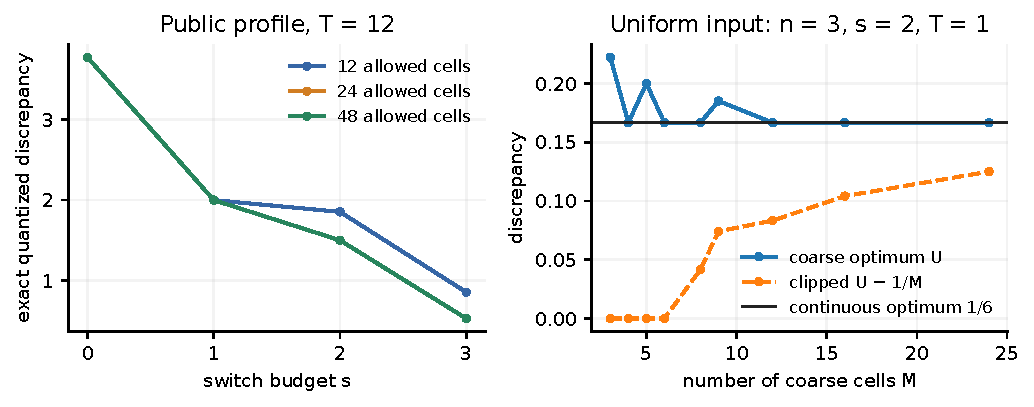
\includegraphics[width=\linewidth]{figures/exact-computations.pdf}
\caption{Left: exact optima on three nested switching grids for the same
quantized public input. Right: coarse upper and clipped lower certificates
for a uniform input with independently known continuous optimum. Lines join
the displayed discrete cases only.}
\label{fig:computations}
\end{figure}

\subsection{Controlled timings and implementation scope}

\newcommand{\FineWall}{0.249}
\newcommand{\FineCPU}{0.246}
\newcommand{\BudgetThreeTwelve}{0.085}
\newcommand{\BudgetThreeTwentyFour}{0.833}
\newcommand{\BudgetThreeFortyEight}{7.980}

Timings use Python 3.13.11 and exact \texttt{Fraction} arithmetic on an Intel
Xeon w5-2565X, Linux under WSL2. Each reported number is the median of three
calls in one process. Inputs are prepared before the timer starts; validation
inside the solver is included, and independent verification afterward is
excluded. Both CPU and wall times and all individual samples are archived.
The host is shared, with no processor affinity or frequency control. These
measurements describe this implementation and workload rather than a general
performance ordering. The full 12,000-cell one-switch solve takes
\FineCPU{} seconds of CPU time and \FineWall{} seconds of wall time.
The three-switch coarse solves take \BudgetThreeTwelve{},
\BudgetThreeTwentyFour{}, and \BudgetThreeFortyEight{} seconds of wall time
for $M=12,24,48$, respectively.

\begin{table}[tb]
\centering\small
\caption{Matched exact methods on deterministic rational inputs. Both methods
optimize the same grid and switch budget. Times are medians in milliseconds;
``words'' counts all labeled-word/boundary cases, including repeated labels.}
\label{tab:controlled-timing}
\begin{tabular}{@{}rrrrrrrr@{}}
\toprule
& & & & \multicolumn{2}{c}{Subset DP} & \multicolumn{2}{c}{Word enumeration}\\
$n$ & $N$ & $s$ & Words & CPU & Wall & CPU & Wall\\
\midrule
3 & 8 & 2 & 567 & 3.85 & 3.82 & 7.48 & 7.42 \\
4 & 8 & 2 & 1344 & 6.67 & 6.62 & 25.44 & 25.25 \\
3 & 8 & 3 & 2835 & 14.02 & 13.92 & 47.71 & 47.36
\\
\bottomrule
\end{tabular}
\end{table}

For Table~\ref{tab:controlled-timing}, cell $j=0,\ldots,N-1$ has width $1/N$
and rates proportional to
$1+\bigl(((j+2)(i+3)+i^2)\bmod 11\bigr)$ for $i=0,\ldots,n-1$. Both methods use exact
rationals, and every optimum agrees. The word enumerator computes endpoint
errors independently rather than calling the subset-cost routine.
This is a controlled comparison with exhaustive enumeration, not with SCARP,
\texttt{pycombina}, or the dwell-constrained heuristic in~\cite{abbasi2025}.

\begin{table}[tb]
\centering\small
\caption{Fixed-budget scaling cases: uniform inputs, horizon one, two switches.
The first four rows vary modes at $N=12$; the remaining rows extend the
$n=8$ grid-size comparison. Times are medians in milliseconds.}
\label{tab:scaling-timing}
\begin{tabular}{@{}rrrr@{}}
\toprule
Modes $n$ & Cells $N$ & CPU & Wall\\
\midrule
4 & 12 & 12.38 & 12.26 \\
8 & 12 & 25.67 & 25.42 \\
16 & 12 & 52.25 & 51.74 \\
32 & 12 & 106.19 & 105.15 \\
8 & 8 & 11.35 & 11.24 \\
8 & 16 & 47.39 & 46.92 \\
8 & 24 & 117.75 & 116.65
\\
\bottomrule
\end{tabular}
\end{table}

Table~\ref{tab:scaling-timing} illustrates the separate mode and grid costs at
fixed budget. The $O(nN^2)$ arithmetic bound for two switches is proved in
Section~\ref{sec:algorithms}; a small timing table cannot establish an
asymptotic complexity claim. Rational bit lengths and interpreter overhead
also affect these measurements. Higher budgets increase the boundary
combinations substantially, which is the reason for using a coarse grid with
an explicit accuracy certificate. The experiments do not solve the underlying
nonlinear Lotka--Volterra optimization problem or measure its trajectory,
objective, or path-constraint performance.

\section{Scope and further questions}\label{sec:discussion}

The results address three different decisions. A minimax formula gives the
worst rounding error before the relaxed input is known. An exact instance
algorithm finds the best schedule once the input is supplied. A coarsening
certificate bounds the loss caused by reducing the allowed switching grid.
Together they separate switch-budget error, grid restriction, and input
representation error, and the minimax analysis imposes no smoothness on the
measurable control.

Two separate Lean developments, listed in the supplement's README, verify
selected results. The \texttt{SwitchingControl} package proves the exact
five-, six-, and seven-cell three-mode values and the continuous value
$F_{3,2}(T)=T/5$, including measurable inputs; it does not cover the chamber
counts, the optimal-switch histograms, or the converse direction of
Proposition~\ref{prop:floor-automaton}. The \texttt{GridSwitching} package
proves the arbitrary-grid one-switch formula, the transfer and coarsening
certificates, and the supporting unrestricted instance algorithms. Their
coverage and verification records specify the proved statements and retained
checks. Neither verifies the whole manuscript, the Python implementations,
timing or bit-cost claims, operation counts beyond candidate-set sizes, or
bibliographic novelty.

Three mathematical extensions remain substantial. First, the exact
five-block one-sided reach bound for general mode count is open. The
exclusion identity in Appendix~\ref{sec:higher-reach} identifies the missing
weighted three-block inequality. The negative event assignment there is not a
control trajectory, and chronological monotonicity removes that particular
obstruction, but a certificate for one chamber covers neither the remaining
orderings nor the full reach bound. The general and seeded results of
Section~\ref{sec:general-budgets} do not depend on this question. A solution
would improve the higher-budget minimax formulas and the second-order
mode-count gap.

Second, the regime with at least as many activation blocks as modes has a
different structure. The three-mode one-sided obstruction rules out a direct
extension of the distinct-mode method, yet the exact value $F_{3,2}(T)=T/5$
and the range $T/7\le F_{3,3}(T)\le T/6$ show that finite-grid chamber methods
can still improve the boundary theory. The floor-history construction is
valid for every grid length, but the enumerations here stop at seven cells.
The six exceptional seven-cell chambers have explicit repairs; their existence
also disproves the tempting unit-error extension on $2s+1$ cells. Determining
$F_{3,3}$ and a general three-mode floor-history switch law requires further
arguments. For other small-mode regimes, the classical
bound~\eqref{eq:classical-small-mode} remains a useful comparison.

Third, constraints beyond a switch budget change the approximation question.
The exact subset algorithm handles its stated per-mode minimum dwell rules,
but a transition graph couples successive labels and is outside that unary
assignment reduction. The odd-grid dwell example shows that unrestricted
coarsening certificates can fail even under arbitrarily fine refinement.
Useful constrained certificates would need assumptions that ensure feasible
nearby switching times, or a constraint-aware refinement construction.

The algorithms already support exact small-budget rounding and certified
additive approximation with rational data. A broader computational study
could compare them with established graph and mixed-integer methods at
matched budgets and objectives, and then evaluate the resulting trajectories
under specified dynamics. Such a study would address application performance,
not the scope of the discrepancy theorems.

\appendix
\section{The remaining higher-block reach question}\label{sec:higher-reach}

No result in the preceding sections assumes an exact reach theorem beyond
four blocks. This appendix states the unresolved step in one proof route
and tests one natural relaxation exactly, separating a failed implication
between linear inequalities from a counterexample generated by an actual
control.

\subsection{An exclusion identity and its missing premise}

Fix $n\ge k+1$, $k\ge3$, $E>0$, and reach maps on $[0,L]$.
For an available set $U$ and $h\le |U|$, let $M_U^h$ be the maximum
reach over all ordered $h$-tuples of distinct elements of $U$.
Write $M^h=M_{[n]}^h$, $M_i^h=M_{[n]\setminus\{i\}}^h$, and
$M_{ij}^h=M_{[n]\setminus\{i,j\}}^h$. These are actual maxima of
reach compositions, not independent event variables. Assume
$M^{k-1}<L$ so every event used below is uncapped.

\begin{lemma}[General exclusion inequality]\label{lem:general-exclusion}
Let $S$ be a $(k-1)$-element set supporting a word attaining $M^{k-1}$.
Then
\begin{align}
 (n-2)M_i^{k-1}
 &\ge nE+M_i^{k-2}+\sum_{j\ne i}M_{ij}^{k-2}-M^{k-1},
       \label{eq:general-exclusion}\\
 \sum_iM_i^{k-1}
 &\ge\left(n-k+1-\frac{k-1}{n-2}\right)M^{k-1}
       +\frac{(k-1)nE+\mathcal H_S^{k-2}}{n-2},
       \label{eq:general-exclusion-sum}\\
 \mathcal H_S^{k-2}
 &:=\sum_{i\in S}\left(M_i^{k-2}+\sum_{j\ne i}M_{ij}^{k-2}\right).
       \label{eq:general-weighted-H}
\end{align}
If also $M^{k-1}\ge B_{k-1}$ and
$\mathcal H_S^{k-2}\ge(k-1)nB_{k-2}$, then $k$ distinct blocks reach
$L$ whenever $L\le B_k$.
\end{lemma}
\begin{proof}
Appending $j$ to a maximizing $(k-2)$-word avoiding $i,j$ gives a
reach no larger than $M_i^{k-1}$. By the uncapped boundary identity
and monotonicity,
\[
 A_j(M_i^{k-1})\le M_i^{k-1}-E-M_{ij}^{k-2}\qquad(j\ne i).
\]
Sum over $j\ne i$ and subtract from conservation to obtain
\[
 A_i(M_i^{k-1})\ge(n-1)E+\sum_{j\ne i}M_{ij}^{k-2}
                              -(n-2)M_i^{k-1}.
\]
Appending $i$ to a maximizing word counted by $M_i^{k-2}$ likewise
gives $A_i(M^{k-1})\le M^{k-1}-E-M_i^{k-2}$.
Since $M_i^{k-1}\le M^{k-1}$, monotonicity of $A_i$ combines these
bounds into~\eqref{eq:general-exclusion}. For $i\notin S$ the same
maximizing word remains available, so $M_i^{k-1}=M^{k-1}$.
Sum~\eqref{eq:general-exclusion} over $i\in S$ and add these equal
outside terms to obtain~\eqref{eq:general-exclusion-sum}.

Its coefficient of $M^{k-1}$ is positive for $n\ge k+1$.
Under the additional premises, use
$n(E+B_{k-2})=(n-1)B_{k-1}$ to deduce
$\sum_iM_i^{k-1}\ge nB_{k-1}$. If no $k$-word reaches $L$, append
$i$ to a maximizing word avoiding $i$. Failure implies the strict
inequality $H_i(L)>M_i^{k-1}+E$. Summing gives
\[
 (n-1)L>\sum_iM_i^{k-1}+nE
             \ge nB_{k-1}+nE=(n-1)B_k,
\]
a contradiction to $L\le B_k$.
\end{proof}

For $k=5$, the premise $M^4\ge B_4$ is already established whenever
$M^4<L$. The missing premise in this route is the weighted three-block
inequality $\mathcal H_S^3\ge4nB_3$ for a maximizing four-mode set
$S$. The stronger statement for every four-element $S$ would suffice
as well. For larger $k$ both the corresponding weighted inequality and
the preceding exact reach induction need justification.
The research question is whether every $n>k\ge5$ measurable input admits
$k$ distinct blocks reaching $\min\{T,B_k(n,E)\}$ for every $E>0$.
If true, it would identify $G^-_{n,k}(T)=TL_{n,k}$ and, by the proved
heavy-mode reduction, the full minimax. The boundary example at $n=k=3$
does not answer it in the spare-mode range.

\subsection{A nonphysical feasible event assignment}\label{subsec:negative-relaxation}

Take $n=6$, $E=1$, label modes $0,\ldots,5$, and fix $S=\{0,1,2,3\}$.
A natural relaxation stores six roots $R_i$ and, for every available set
$U$ of size at least three, a pair event $(2,U)$; for every $|U|\ge4$
it stores a triple event $(3,U)$. Each event $v$ has time $t_v$ and
six allocations $a_{v,i}$. There are 42 pair events and 22 triple events,
hence $6+7\cdot64=454$ nonnegative variables. The full row specification is
\begin{align*}
 &R_i\ge1,\quad R_0\le R_i\ (i\ne0),\quad\sum_{i\ne0}R_i\ge6,\\
 &\sum_i a_{v,i}=t_v,\quad a_{(h,U),i}\ge R_i-1\quad(i\in U),\\
 &t_{(2,U)}-a_{(2,U),i}\ge R_j+1\quad(i,j\in U,\ i\ne j),\\
 &t_{(3,U)}-a_{(3,U),i}\ge t_{(2,U\setminus\{i\})}+1\quad(i\in U),\\
 &a_{(h,U),i}\le a_{(h',U'),i}
       \quad(h\le h',\ U\subseteq U',\ (h,U)\ne(h',U')),\\
 &a_{(h,[6]),i}\le a_{(h,U),i}
       \quad(P_h\subseteq U\ne[6]),
       \qquad P_2=\{0,1\},\ P_3=\{0,1,2\}.
\end{align*}
Here $[6]$ denotes all six labels in this subsection. The last rows and
the inclusion rows together force equality for events sharing the fixed
global maximizing pair or triple. Each row is necessary for actual
uncapped events with those maximizers and with $R_0$ smallest. Indeed,
adding available modes or activation blocks cannot decrease maximum reach,
and coordinate allocations increase with time. In the all-available
three-block objective define
\[
 \mathcal H_S^3=\sum_{i\in S}\left(t_{(3,[6]\setminus\{i\})}
               +\sum_{j\ne i}t_{(3,[6]\setminus\{i,j\})}\right).
\]
The bundled rational assignment satisfies all 3660 displayed inequalities
and all 64 conservation equalities, with nonnegative variables, but gives
\begin{equation}\label{eq:negative-event-objective}
 \mathcal H_S^3=\frac{40328}{387}<\frac{13104}{125}=4nB_3(6,1).
\end{equation}
Both a row-matrix checker and an independently organized event checker
verify these facts exactly. Thus these necessary constraints do not imply
the proposed weighted inequality for arbitrary four-element $S$.

This is not a counterexample to any reach theorem. The pair event for
$U=\{0,2,3\}$ has time $1658/645$; that for $V=\{2,3,4,5\}$ has
the later time $614/215$. Yet the corresponding mode 2 allocation falls
from $239/645$ to $47/129$. The time difference is $184/645>0$ and
the allocation drop is $4/645>0$. The sets are incomparable by inclusion,
so the relaxation omitted this chronological comparison. A common
cumulative control cannot produce these data. Nor does the relaxation
require $S$ itself to support a global maximizing four-word, a further
condition if one only seeks the weaker premise in
Lemma~\ref{lem:general-exclusion}.

\begin{lemma}[Interpolation of event allocations]\label{lem:event-interpolation}
Let finitely many events $(t_v,a_v)$ have $t_v\ge0$, $a_v\in\R_+^n$,
and $\sum_i a_{v,i}=t_v$. They lie on a common admissible cumulative
trajectory if and only if
\begin{equation}\label{eq:chronological-order}
 t_v\le t_w\quad\Longrightarrow\quad a_{v,i}\le a_{w,i}
                    \quad\hbox{for every }i.
\end{equation}
Such a trajectory can be chosen piecewise affine, up to and beyond the
last event.
\end{lemma}
\begin{proof}
Necessity follows from coordinate monotonicity. For sufficiency, sort the
events by time and add $(0,0)$. Equal-time allocations agree because
coordinate order in both directions forces equality; equivalently,
nonnegative ordered differences with zero total are zero. Between distinct
successive times interpolate linearly. Each coordinate increment is
nonnegative and their sum is the time increment, so the slope vector is
simplex-valued. Extend after the last event with any simplex-valued constant
rate. This gives an admissible trajectory containing all event data.
\end{proof}

This lemma concerns interpolation only. For actual reach events, the
variables $R_i,t_{h,U}$ must also equal the specified latest inverse and
maximum-composition reaches of that same trajectory; conservation and
chronological interpolation alone do not establish these identities.

\subsection{An exact chronological-chamber test}\label{subsec:chronological-test}

We strengthen the failed relaxation by sorting its 64 events in the
nondecreasing time order of the saved witness. Ties are resolved by their
original enumeration: first order $h=2,3$, then decreasing $|U|$, then
lexicographic order of the increasing mode tuples. Let $v_1,\ldots,v_{64}$
be that fixed permutation. Add the 378 inequalities
\begin{equation}\label{eq:chamber-cuts}
 a_{v_j,i}\le a_{v_{j+1},i}\qquad(1\le j<64,\ 0\le i<6).
\end{equation}
Conservation then also forces $t_{v_j}\le t_{v_{j+1}}$.
Thus this is one closed chronological chamber, allowing ties, not a
global imposition of the old witness's numerical times. The witness itself
has 239 violations of ordered coordinate comparisons, with largest drop
$224/645$, and is excluded by these new rows.

\begin{proposition}[One strengthened chamber, computer-assisted]
\label{prop:chronological-chamber}
For this single fixed event permutation, the strengthened relaxation with
454 variables, 4038 inequalities, and 64 equalities has exact minimum
\[
 \min\mathcal H_S^3=13104/125=4nB_3(6,1).
\]
\end{proposition}
\begin{proof}
Write the inequalities as $Ax\le b$, the equalities as $Qx=d$, and
the objective as $c^\top x$, with $x\ge0$. The supplement supplies
rational vectors $y,z$ and verifies, component by component,
\[
 y\le0,\qquad c-A^\top y-Q^\top z\ge0,\qquad
 b^\top y+d^\top z=13104/125.
\]
Consequently every feasible $x$ satisfies
$c^\top x\ge y^\top Ax+z^\top Qx\ge b^\top y+d^\top z$.
There are 254 nonzero dual rows; the checker reconstructs every integer
row from the bundled original relaxation and the explicit permutation,
then sorts normalized sparse rows and their right-hand sides
lexicographically before applying the dual vectors.
It uses only rational arithmetic and does not invoke a numerical solver.

For attainment, take $R_i=6/5$, every pair-event time $66/25$, every
triple-event time $546/125$, and $a_{v,i}=t_v/6$. These are precisely the
uniform-control events. In the chosen permutation all pair events precede
all triple events, so every chamber row holds. All original rows and the
objective equality are verified exactly as well. There are 24 triple-time
terms in the objective, giving $24(546/125)=13104/125$.
\end{proof}

The exact certificate closes the relaxation gap in this chamber. It does
not cover the other chronological permutations, other choices of global
maximizers, or other mode counts, and it does not assert that every point
in the strengthened relaxation satisfies the inverse reach identities.
A floating-point linear program was used only to discover the rational
dual; the proof is the checked rational identity and the matching explicit
primal. The general five-block reach problem remains open. Separately, a
possible strengthening of Lemma~\ref{lem:first-repeat} that forces an
adjacent pair of a largest heavy mode is unproved and unused; the
existential heavy-mode theorem does not depend on it.

\bibliographystyle{plainnat}
\bibliography{references}
\end{document}
